\documentclass[12pt,a4paper,twoside,openany]{book}

\newcommand{\ThesisTitle}{Detección y seguimiento automático de microorganismos acuáticos para el análisis de su cinemática en función de la temperatura}
\newcommand{\ThesisAuthor}{Alexis Tomas Centeno}
\newcommand{\ThesisDegree}{Licenciatura en Ciencias de la Computación}
\newcommand{\ThesisFaculty}{Facultad de Matemática, Astronomía, Física y Computación}
\newcommand{\ThesisUniversity}{Universidad Nacional de Córdoba}

% Completar antes de la entrega final:
\newcommand{\ThesisAdvisor}{Directora: Debora Analia Pedernera}
\newcommand{\ThesisDate}{Mes, 2026}

\usepackage[english,spanish,es-nodecimaldot,es-lcroman]{babel}
\usepackage{amsmath,amssymb,mathtools}
\usepackage{fontspec}
% RHCD 572/2024, art. 1: no sustituir silenciosamente la fuente exigida.
\IfFontExistsTF{Times New Roman}{
  \setmainfont{Times New Roman}
}{
  \IfFontExistsTF{Arial}{
    \setmainfont{Arial}
  }{
    \PackageError{tesis}{Instale Times New Roman o Arial}{La RHCD 572/2024 exige una de estas fuentes.}
  }
}
\usepackage{microtype}
\setlength{\emergencystretch}{3em}
\usepackage[a4paper,left=30mm,right=25mm,top=25mm,bottom=25mm]{geometry}
\usepackage{emptypage}
\usepackage{setspace}
\singlespacing

\usepackage{siunitx}
\sisetup{output-decimal-marker={,}}

\usepackage{graphicx}
\usepackage{float}
\usepackage{listings}
\lstdefinestyle{thesiscode}{
  basicstyle=\ttfamily\footnotesize,
  columns=fullflexible,
  keepspaces=true,
  breaklines=true,
  breakatwhitespace=true,
  showstringspaces=false,
  frame=single,
  framerule=0.3pt,
  xleftmargin=3mm,
  xrightmargin=3mm,
  aboveskip=0.8em,
  belowskip=0.8em
}
\usepackage{booktabs}
\usepackage{longtable}
\usepackage{tabularx}
\usepackage{caption}
\usepackage{subcaption}

\usepackage{tikz}
\usetikzlibrary{arrows.meta,positioning,fit}

\usepackage{xcolor}
\usepackage{hyperref}
\usepackage[nameinlink,noabbrev]{cleveref}
\hypersetup{
  hidelinks,
  pdftitle={\ThesisTitle},
  pdfauthor={\ThesisAuthor}
}

\usepackage{csquotes}
\usepackage[
  backend=biber,
  style=numeric,
  sorting=none,
  maxbibnames=99,
  giveninits=true
]{biblatex}
\addbibresource{bibliography/references.bib}

\usepackage{titlesec}
\titleformat{\chapter}[display]
  {\normalfont\bfseries\LARGE\raggedright}
  {\chaptertitlename\ \thechapter}
  {0.5em}
  {\Huge}
\titleformat{\section}
  {\normalfont\Large\bfseries\raggedright}
  {\thesection}{1em}{}
\makeatletter
\renewcommand*\l@section{\@dottedtocline{1}{1.5em}{3em}}
\renewcommand*\l@subsection{\@dottedtocline{2}{4.5em}{3.2em}}
\makeatother
\titleformat{\subsubsection}
  {\normalfont\bfseries\normalsize}
  {}
  {0pt}
  {}

\setcounter{secnumdepth}{2}
\setcounter{tocdepth}{2}

\usepackage{fancyhdr}
\pagestyle{fancy}
\fancyhf{}
\fancyfoot[C]{\thepage}
\renewcommand{\headrulewidth}{0pt}


% Evita estirar los espacios entre bloques para igualar la altura de las páginas.
\raggedbottom

\newcommand{\thesisgraphic}[2][0.9\textwidth]{%
  \IfFileExists{#2}{%
    \includegraphics[width=#1]{#2}%
  }{%
    \fbox{\parbox[c][4cm][c]{#1}{\centering
      Figura pendiente de renderizado\\[0.4em]
      \texttt{\detokenize{#2}}}}%
  }%
}

\newcommand{\institutionlogo}[2][0.26\textwidth]{%
  \IfFileExists{#2}{%
    \includegraphics[width=#1]{#2}%
  }{%
    \fbox{\parbox[c][1.4cm][c]{#1}{\centering Logo pendiente}}%
  }%
}


% Estilo común para diagramas metodológicos.
\tikzset{
  thesisflow/.style={
    draw,
    rounded corners=2pt,
    align=center,
    inner xsep=6pt,
    inner ysep=4pt,
    font=\small
  },
  thesisarrow/.style={
    -{Latex[length=2mm]},
    line width=0.55pt
  },
  thesisgroup/.style={
    draw=gray,
    rounded corners=2pt,
    inner sep=5pt
  }
}


% Una hoja de guarda equivale a dos carillas sin impresión.
\newcommand{\thesisguardleaf}{%
  \clearpage
  \null\thispagestyle{empty}\newpage
  \null\thispagestyle{empty}\newpage
}


% El borrador no incorpora páginas de guarda ni separadores en blanco.
\ifThesisFinalLayout\else
  \let\cleardoublepage\clearpage
\fi

\begin{document}

\ifThesisFinalLayout
  \hypersetup{pageanchor=false}
  \thesisguardleaf
\fi
\frontmatter
\hypersetup{pageanchor=true}
\begin{titlepage}
\centering

\begin{minipage}[t]{0.49\textwidth}
  \raggedright
  \institutionlogo[0.60\textwidth]{assets/logos/unc.png}
\end{minipage}
\hfill
\begin{minipage}[t]{0.49\textwidth}
  \raggedleft
  \institutionlogo[0.60\textwidth]{assets/logos/famaf.png}
\end{minipage}

\vspace{2.8cm}

{\Large\bfseries \ThesisTitle\par}

\vspace{1.4cm}

{\large por\par}
\vspace{0.25cm}
{\Large \ThesisAuthor\par}

\vspace{2cm}

Trabajo presentado ante la \ThesisFaculty\\
como parte de los requisitos para la obtención del grado de\\
\textbf{\ThesisDegree}

\vspace{1.2cm}

{\bfseries \ThesisUniversity\par}

\vspace{1cm}

\ThesisDate

\vfill

\ThesisAdvisor

\end{titlepage}

\chapter*{Resumen}
\addcontentsline{toc}{chapter}{Resumen}

A principios de 2024 se abrió una línea de investigación dentro del Grupo de Física de la Atmósfera orientada a indagar la posible existencia de vida microbiana en venas líquidas del hielo \cite{mader2006,rohde2007,dani2012}. En sus primeras etapas se estudió el movimiento de microorganismos de aguas estancadas de Córdoba entre 0 °C y 15 °C, con interés en su actividad cerca del punto de fusión del hielo \cite{pedernera2024}. Las grabaciones se adquirieron con una cámara acoplada a un microscopio óptico. El estudio de sus trayectorias y rapideces medias, y su posible relación con la temperatura, motivó la necesidad de obtener mediciones individuales; en las muestras iniciales se distinguieron cuatro tipos de microorganismos.

La reconstrucción manual de trayectorias mediante Tracker requiere registrar posiciones en numerosos cuadros. Para apoyar ese análisis, esta tesis desarrolló un sistema de visión por computadora que integra un detector YOLO11 adaptado al material disponible, el seguimiento mediante BoT-SORT y el registro de posiciones por identificador. A partir de esas posiciones calcula distancias, rapidez, variaciones de rapidez e indicadores temporales, aplica una clasificación de patrones basada en reglas y genera productos de inspección.

La evaluación comprende los registros de dos entrenamientos, pruebas controladas y la comparación de una trayectoria automática con una referencia manual parcial de \texttt{primer\_minuto.mp4}, video identificado por confirmación del autor. Tras alinear los sistemas de coordenadas con un anclaje inicial, las 92 posiciones posteriores comparadas presentaron una separación media de $5{,}33$ px. La comparación de rapidez mostró discrepancias que requieren una evaluación diferenciada de las magnitudes derivadas. Las verificaciones numéricas respaldaron el uso de los intervalos reales entre cuadros en los casos examinados.

El aporte computacional consiste en integrar y adaptar el procesamiento al material de esta línea experimental. La evidencia de seguimiento se limita al caso estudiado; quedan pendientes su ampliación, la validación independiente de las categorías y la medición del ahorro de tiempo. La tesis no evalúa efectos de temperatura sobre el movimiento. Las mediciones se conservan en px, px/s y px/s$^2$; la calibración óptica y la conversión a unidades físicas corresponden a una etapa externa al alcance del trabajo.

\chapter*{Abstract}
\addcontentsline{toc}{chapter}{Abstract}

\begin{otherlanguage}{english}
This thesis presents a computer vision system for detecting, tracking, and analyzing the motion of aquatic microorganisms in videos acquired through optical microscopy. The work supports an experimental research line within the Atmospheric Physics Group that studies microorganisms from stagnant water samples collected in Córdoba under varying temperatures, between 0 °C and 15 °C \cite{pedernera2024}. Manual trajectory reconstruction using Tracker motivated the development of an automated procedure to organize positions and measurements for subsequent inspection.

The system integrates a YOLO11 detector adapted to the available material, multi-object tracking with BoT-SORT, and position recording by identifier. From the reconstructed trajectories, it computes distances, speed, changes in speed, and temporal continuity, identifies low-mobility samples, and applies a rule-based classification of motion patterns. Plots, annotated videos, and result files support inspection of associations and calculated quantities.

The evaluation includes records from two detector training runs, controlled numerical and integration tests, and a comparison between one automated trajectory and a partial manual reference. After aligning the coordinate systems using an initial anchor, the 92 subsequent matched positions had a mean separation of $5.33$ px. Numerical checks confirmed, for the examined cases, the use of actual frame intervals, including gaps in position records. Speed comparisons showed that spatial similarity must be assessed alongside discrepancies in derived quantities.

The contribution lies in integrating and adapting the processing workflow to the experimental material of this research line. The available evidence is limited to the evaluated cases; broader tracking evaluation, independent validation of motion categories, and measurement of time savings remain pending. Temperature provides the experimental context, and its effect on kinematics is not evaluated in this thesis. Quantities are expressed in px, px/s, and px/s$^2$; spatial calibration and conversion to physical units remain \textbf{TO BE DEFINED}.
\end{otherlanguage}



\tableofcontents
\listoffigures
\listoftables

\mainmatter
\chapter{Introducción}

\section{Contexto general}

A principios de 2024 se inició, dentro del Grupo de Física de la Atmósfera (GFA), una línea de investigación orientada al estudio de la posible existencia de vida microbiana en las venas líquidas presentes en el hielo \cite{mader2006,rohde2007,dani2012}. Esta línea busca contribuir a la comprensión de la capacidad de los microorganismos para sobrevivir y mantener actividad biológica en ambientes caracterizados por temperaturas cercanas al punto de congelación y otras condiciones físicas potencialmente adversas.

Como primera aproximación experimental, la investigación se centró en microorganismos acuáticos presentes en muestras de aguas estancadas de la ciudad de Córdoba. Estas muestras fueron estudiadas en un rango de temperaturas comprendido entre 0 °C y 15 °C, con el propósito de observar su comportamiento en condiciones progresivamente cercanas al punto de fusión del hielo. Este enfoque permite analizar posibles variaciones en la movilidad de los microorganismos y obtener información relacionada con su actividad en entornos de baja temperatura \cite{pedernera2024}.

Las observaciones experimentales se realizaron mediante videos adquiridos con una cámara acoplada a un microscopio óptico. A partir de estas grabaciones, los investigadores de esta línea experimental comenzaron a estudiar las trayectorias descriptas por los microorganismos, sus rapideces medias y la posible relación de estas magnitudes con la temperatura del medio acuático. En las muestras consideradas durante las primeras etapas de la investigación se identificaron cuatro tipos de microorganismos, cuyos movimientos requieren ser observados y cuantificados individualmente.

En este contexto, el análisis cuantitativo del movimiento constituye una herramienta para comparar la actividad observada bajo distintas condiciones experimentales. El presente trabajo aborda, por lo tanto, la necesidad de procesar de manera sistemática los videos obtenidos durante los experimentos y transformar las observaciones visuales en datos cuantitativos que puedan ser analizados posteriormente.

\section{Motivación del trabajo}

La caracterización del movimiento requiere reconstruir trayectorias individuales y calcular magnitudes como la distancia recorrida, la rapidez y sus variaciones, junto con indicadores de continuidad y baja movilidad. La aplicación de criterios uniformes permite organizar estas mediciones para comparar individuos, muestras y condiciones experimentales.

Automatizar el registro de posiciones y su análisis puede reducir la intervención manual y facilitar el procesamiento de más grabaciones. Esta posibilidad motiva el trabajo y permitiría concentrar la participación de los investigadores en la revisión e interpretación de los resultados. Su utilidad práctica debe cuantificarse mediante una comparación del esfuerzo total de análisis.

\section{Problema general}

En la línea experimental que da origen a esta tesis, las trayectorias se reconstruían manualmente con Tracker: un operador identificaba cada microorganismo y registraba su posición en numerosos cuadros. El esfuerzo aumenta al incorporar individuos, muestras y repeticiones, y la selección de posiciones puede variar entre anotaciones. Los cruces, el bajo contraste y los desplazamientos rápidos dificultan además reconocer al mismo individuo durante toda la secuencia.

El problema abordado es disponer de un procedimiento automático, adaptado y evaluado para estas grabaciones, que transforme las posiciones de múltiples microorganismos en trayectorias y mediciones revisables. El capítulo 2 precisa las unidades de análisis y el alcance de ese procesamiento.

\section{Propuesta del trabajo}

En esta tesis se desarrolló un sistema de visión por computadora, denominado en adelante \emph{el sistema}, para procesar videos adquiridos mediante microscopía óptica. Integra la localización de microorganismos, la asociación de sus detecciones y la reconstrucción de trayectorias. Conservar la identidad temporal significa asociar las posiciones de un mismo individuo entre cuadros. La continuidad temporal describe la presencia de posiciones registradas dentro del intervalo de seguimiento; una trayectoria continua carece de cuadros intermedios sin registro, denominados \emph{gaps}. Un mismo identificador puede conservarse a ambos lados de un gap, por lo que identidad y continuidad son propiedades distintas.

A partir de las trayectorias, el sistema calcula desplazamientos, rapidez y variaciones de rapidez, junto con indicadores de baja movilidad y continuidad. También aplica una clasificación interpretable de patrones básicos de movimiento y genera visualizaciones, videos procesados y archivos de resultados para su inspección posterior.

La evaluación presentada considera los registros de entrenamiento del detector, la comparación de una trayectoria automática con una referencia manual parcial y la consistencia de las magnitudes calculadas. Las pruebas controladas complementan ese análisis mediante la verificación de cálculos e integración. La reducción del tiempo de trabajo constituye una motivación de la propuesta y queda pendiente de mediciones comparables.

El sistema proporciona mediciones organizadas mediante criterios reproducibles para su interpretación por parte de los especialistas. La temperatura caracteriza el contexto experimental de esta línea de investigación; la evaluación de la tesis se concentra en el procesamiento computacional y no compara el movimiento entre temperaturas ni determina sus efectos físicos o biológicos.

\section{Organización de la tesis}

La tesis se organiza en doce capítulos, un apéndice y las referencias bibliográficas. El presente capítulo introduce el contexto científico, la motivación, el problema general y la propuesta del trabajo. El capítulo 2 delimita el problema de investigación, define las unidades de análisis y las magnitudes de interés, y establece el alcance del estudio. El capítulo 3 desarrolla la perspectiva teórica y los antecedentes relacionados con la visión por computadora, la detección, el seguimiento y el análisis de trayectorias. El capítulo 4 describe el diseño metodológico utilizado para desarrollar y evaluar el sistema.

Los capítulos 5 a 10 presentan el desarrollo computacional del sistema. El capítulo 5 describe su arquitectura y organización general; el capítulo 6 aborda la detección automática de microorganismos; el capítulo 7 desarrolla el seguimiento y la reconstrucción de trayectorias; el capítulo 8 presenta las métricas utilizadas para analizar el movimiento; el capítulo 9 explica el método de clasificación de patrones; y el capítulo 10 documenta la implementación y las pruebas realizadas.

Finalmente, el capítulo 11 integra la evaluación experimental, los resultados obtenidos y su discusión, considerando los aportes y las limitaciones del sistema. El capítulo 12 reúne las conclusiones y las líneas de trabajo futuro. El Apéndice~\ref{ap:guia-ejecucion} presenta las instrucciones de ejecución e inspección, los formatos de salida y la reproducción de las verificaciones y figuras.

\chapter{Planteamiento del problema de investigación}

Este capítulo delimita el problema de investigación desde una perspectiva computacional y cuantitativa. Para ello, se definen las unidades de análisis y las magnitudes observadas, y se establece el alcance del estudio. La investigación se centra en evaluar el sistema para obtener mediciones del movimiento a partir de videos adquiridos mediante microscopía óptica, sin abordar directamente la interpretación física o biológica de los resultados.

\section{Delimitación del problema}

El trabajo se delimita al desarrollo y evaluación del sistema para procesar videos previamente adquiridos en la línea experimental del GFA presentada en el capítulo 1. La entrada es la secuencia de imágenes; la salida comprende posiciones asociadas por individuo, trayectorias, métricas y productos de inspección.

El problema computacional combina la localización de varios microorganismos con la asociación de sus detecciones entre cuadros. La asociación debe representar a un mismo individuo a lo largo del seguimiento, incluso cuando se producen pérdidas temporales de detección. La calidad de estas dos etapas condiciona las mediciones posteriores.

La temperatura se conserva como información contextual de cada grabación. La evaluación presentada comprende los registros de entrenamiento, pruebas controladas y una comparación de trayectoria con una referencia manual parcial; no incluye una comparación del movimiento entre condiciones térmicas. Los resultados corresponden al material y las configuraciones documentados, cuya resolución, frecuencia de cuadros, iluminación y contraste condicionan el desempeño.

\section{Unidad de análisis}

En este trabajo se distinguen tres niveles relacionados de análisis: el microorganismo observado, la trayectoria reconstruida y el video experimental.

\subsection{Unidad primaria de análisis}

La unidad primaria de análisis es cada microorganismo acuático identificado y seguido dentro de un video adquirido mediante microscopía óptica. Desde el punto de vista computacional, cada microorganismo se representa mediante un identificador de seguimiento, denominado track ID, que permite asociar las detecciones obtenidas en distintos cuadros y considerarlas como registros de un mismo individuo.

La identidad temporal expresa la hipótesis de que las detecciones asociadas pertenecen a un mismo individuo. Es una identificación visual y operativa. El sistema reconoce objetos compatibles con las clases incluidas en los datos de entrenamiento, pero no realiza una identificación taxonómica ni determina propiedades biológicas de los microorganismos. Además, la correspondencia entre un identificador computacional y un individuo real depende de la calidad de la detección y del seguimiento.

\subsection{Unidad secundaria de análisis}

La unidad secundaria de análisis es la trayectoria reconstruida para cada microorganismo: la sucesión ordenada de sus posiciones estimadas en el plano de la imagen. Cada posición conserva el número de cuadro correspondiente, necesario para ubicarla en el tiempo y calcular las magnitudes de movimiento.

El video registra muestras discretas de ese recorrido. Su representación computacional y su relación con la función posición se formalizan en la sección siguiente. La calidad de la trayectoria depende de la localización del microorganismo y de la conservación de su identidad; las pérdidas de detección y las asociaciones incorrectas pueden afectar las métricas derivadas.

\subsection{Unidad experimental}

La unidad experimental es cada video adquirido mediante microscopía óptica bajo una determinada condición de observación. El video contiene la secuencia de imágenes sobre la que se ejecutan las etapas de detección, seguimiento y análisis de trayectorias.

Cada grabación se encuentra asociada con una muestra, una temperatura y determinadas condiciones de adquisición. Dentro de un mismo video pueden detectarse y seguirse varios microorganismos, por lo que es posible obtener métricas individuales y posteriormente construir indicadores generales para la grabación.

La Figura~\ref{fig:unidades-analisis} resume la relación entre las unidades de análisis y las métricas obtenidas para cada trayectoria.

\begin{figure}[H]
  \centering
  \begin{tikzpicture}[
    x=1cm,
    y=1cm,
    box/.style={thesisflow,text width=2.65cm,minimum height=1cm,font=\footnotesize},
    heading/.style={align=center,text width=2.9cm,font=\footnotesize\bfseries},
    every node/.style={outer sep=0pt}
  ]
    \node[heading] at (0,1.9) {Unidad\\experimental};
    \node[heading] at (3.6,1.9) {Unidad\\primaria};
    \node[heading] at (7.2,1.9) {Unidad\\secundaria};
    \node[heading] at (10.8,1.9) {Magnitudes\\derivadas};

    \node[box] (video) at (0,0) {Video adquirido\\mediante microscopía óptica};
    \node[box] (organismo-a) at (3.6,0.7) {Microorganismo\\A};
    \node[box] (organismo-b) at (3.6,-0.7) {Microorganismo\\B};
    \node[box] (trayectoria-a) at (7.2,0.7) {Trayectoria A};
    \node[box] (trayectoria-b) at (7.2,-0.7) {Trayectoria B};
    \node[box] (metricas-a) at (10.8,0.7) {Métricas de A};
    \node[box] (metricas-b) at (10.8,-0.7) {Métricas de B};

    \draw[thesisarrow] (video.east) -- ++(0.25,0) |- (organismo-a.west);
    \draw[thesisarrow] (video.east) -- ++(0.25,0) |- (organismo-b.west);
    \draw[thesisarrow] (organismo-a.east) -- (trayectoria-a.west);
    \draw[thesisarrow] (organismo-b.east) -- (trayectoria-b.west);
    \draw[thesisarrow] (trayectoria-a.east) -- (metricas-a.west);
    \draw[thesisarrow] (trayectoria-b.east) -- (metricas-b.west);
  \end{tikzpicture}
  \caption{Relación entre las unidades de análisis. Un mismo video permite observar varios microorganismos y obtener sus trayectorias y métricas individuales. Los individuos A y B se muestran a modo esquemático.}
  \label{fig:unidades-analisis}
\end{figure}

\section{Variables y magnitudes de interés}

El estudio adopta un enfoque cuantitativo basado en variables asociadas con el desplazamiento de los microorganismos y con las condiciones de adquisición de los videos. Estas variables se dividen en dos grupos: variables computacionales, obtenidas mediante el procesamiento de las trayectorias, y variables experimentales o contextuales, utilizadas para interpretar y organizar los resultados.

\subsection{Variables computacionales y métricas de movimiento}

\subsubsection{Posición registrada}

La posición representa la ubicación estimada de un microorganismo en un cuadro determinado del video. Para el cuadro $f_i$, se expresa mediante el par de coordenadas:

\nopagebreak[4]
\[
\vec{p}_i=(x_i,y_i).
\]

donde $x_i$ e $y_i$ corresponden al centro de la caja delimitadora obtenida mediante el detector.

Las coordenadas se expresan en píxeles, unidad espacial de la imagen. La calibración y su conversión a unidades físicas permanecen \textbf{A DEFINIR}.

\subsubsection{Relación entre cuadro y tiempo}

El número de cuadro $f_i\in\mathbb{N}_0=\{0,1,2,\ldots\}$ es un índice discreto. El subíndice $i$ enumera los registros de una trayectoria, mientras que $f_i$ identifica el cuadro del video; por ello, los valores de $f_i$ pueden presentar saltos. La frecuencia de cuadros se expresa en cuadros por segundo (FPS, por sus siglas en inglés, \emph{frames per second}).

Con el primer cuadro numerado como cero y el origen temporal en el inicio del video, el instante asociado con cada registro es
\[
t_i=\frac{f_i}{FPS}.
\]
Si se elige otro cuadro $f_0$ como origen, se utiliza $t_i=(f_i-f_0)/FPS$. Esta elección cambia la referencia temporal, pero conserva el intervalo entre dos registros:
\[
\Delta t_i=\frac{f_{i+1}-f_i}{FPS}.
\]
La conversión expresa los tiempos en segundos y conserva los cuadros realmente transcurridos, incluidos aquellos sin posición registrada.

\subsubsection{Secuencia ordenada de observaciones}

Para cada identificador de seguimiento, el sistema almacena una secuencia ordenada de observaciones:

\[
\mathcal{O}=\left\{(f_i,\vec{p}_i)\right\}_{i=1}^{n},
\qquad \vec{p}_i=(x_i,y_i).
\]

Cada elemento contiene el número de cuadro y la posición estimada del microorganismo. Esta secuencia constituye la representación computacional directamente obtenida del proceso de seguimiento.

Los cuadros registrados no necesariamente son consecutivos. Las pérdidas temporales de detección o las dificultades de asociación pueden producir intervalos sin observaciones, denominados gaps.

\subsubsection{Función posición y trayectoria}

Desde una perspectiva cinemática, el movimiento puede describirse mediante una función posición:

\[
\vec{r}(t)=\bigl(x(t),y(t)\bigr),
\]

que representa la ubicación del microorganismo en función del tiempo.

El sistema registra posiciones en instantes discretos: $\vec{r}(t_i)=\vec{p}_i=(x_i,y_i)$. Estas muestras aproximan el recorrido en el plano de la imagen; la función continua sirve como referencia conceptual.

La trayectoria corresponde al recorrido geométrico descripto por el microorganismo. En el sistema se aproxima mediante la sucesión ordenada de las posiciones registradas:

\[
\mathcal{T}=(\vec{p}_1,\vec{p}_2,\ldots,\vec{p}_n).
\]

Esta distinción permite separar conceptualmente la información espacial correspondiente al recorrido de la información temporal que indica cómo dicho recorrido se desarrolla a lo largo del video.

\subsubsection{Duración del seguimiento}

La duración del seguimiento corresponde al tiempo transcurrido entre la primera y la última observación asociada con un mismo identificador:

\[
T=t_n-t_1.
\]

Utilizando directamente los números de cuadro, puede calcularse como:

\[
T=\frac{f_n-f_1}{FPS}.
\]

La duración temporal debe distinguirse de la cantidad de observaciones disponibles. Una trayectoria puede extenderse durante un intervalo prolongado y, al mismo tiempo, contener pérdidas temporales de detección.

Por esta razón, la cantidad de observaciones y la duración constituyen propiedades diferentes y deben analizarse conjuntamente con las métricas de continuidad temporal.

\subsubsection{Distancia total recorrida}

La distancia total recorrida representa la longitud acumulada del desplazamiento reconstruido a partir de las posiciones observadas del microorganismo.

Sean dos posiciones consecutivas de la trayectoria $\vec{p}_i$ y $\vec{p}_{i+1}$, la distancia correspondiente al segmento comprendido entre ambas posiciones se calcula mediante la distancia euclídea:

\[
d_i=\left\|\vec{p}_{i+1}-\vec{p}_i\right\|.
\]

o, expresada en coordenadas:

\[
d_i=\sqrt{(x_{i+1}-x_i)^2+(y_{i+1}-y_i)^2}.
\]

Para una trayectoria formada por n posiciones observadas, la distancia total recorrida se obtiene sumando las distancias de los n-1 segmentos consecutivos:

\[
D_T=\sum_{i=1}^{n-1}d_i
=\sum_{i=1}^{n-1}\left\|\vec{p}_{i+1}-\vec{p}_i\right\|.
\]

Esta magnitud permite estimar la longitud total del recorrido reconstruido, independientemente de la dirección seguida por el microorganismo.

\subsubsection{Desplazamiento neto}

La distancia neta representa la separación entre la posición inicial y la posición final de la trayectoria. En este trabajo se utiliza su magnitud:

\[
D_N=\left\|\vec{p}_n-\vec{p}_1\right\|.
\]

A diferencia de la distancia total, esta magnitud no considera el recorrido intermedio. La comparación entre la distancia total y la magnitud del desplazamiento neto permite obtener información sobre la geometría general de la trayectoria. Por ejemplo, una trayectoria que regresa aproximadamente a su punto de partida puede presentar una distancia total elevada y, al mismo tiempo, un desplazamiento neto reducido.

\subsubsection{Velocidad y rapidez entre observaciones}

La velocidad es una magnitud vectorial. Esto significa que indica no solo cuánto se mueve el microorganismo, sino también en qué dirección y sentido.

La velocidad media correspondiente al tramo entre ambas observaciones se estima mediante:

\[
\vec{v}_i=\frac{\vec{p}_{i+1}-\vec{p}_i}{\Delta t_i}.
\]

Como las posiciones tienen dos coordenadas, puede escribirse:

\[
\vec{v}_i=
\left(
\frac{x_{i+1}-x_i}{\Delta t_i},
\frac{y_{i+1}-y_i}{\Delta t_i}
\right).
\]

Por lo tanto, sus componentes son:

\[
v_{x,i}=\frac{x_{i+1}-x_i}{\Delta t_i}.
\]

\[
v_{y,i}=\frac{y_{i+1}-y_i}{\Delta t_i}.
\]

El signo de cada componente depende del sentido del desplazamiento y de la orientación de los ejes. En las coordenadas de imagen utilizadas por el sistema, el eje vertical crece hacia abajo.

La rapidez no conserva la dirección. Es una magnitud escalar que indica únicamente cuánto se desplaza el microorganismo por unidad de tiempo.

Se obtiene calculando el módulo de la velocidad:

\[
v_i=\left\|\vec{v}_i\right\|
=\frac{\left\|\vec{p}_{i+1}-\vec{p}_i\right\|}{\Delta t_i}.
\]

En términos de los números de cuadro, la rapidez se expresa como:

\[
v_i=
\frac{\left\|\vec{p}_{i+1}-\vec{p}_i\right\|\,FPS}
{f_{i+1}-f_i}.
\]

\subsubsection{Velocidad media y rapidez media de una trayectoria}

La velocidad media y la rapidez media describen propiedades diferentes del movimiento de un microorganismo a lo largo de una trayectoria completa.

La velocidad media es una magnitud vectorial y se calcula a partir del desplazamiento neto entre la posición inicial y la posición final, dividido por el tiempo total transcurrido:

\[
\overline{\vec{v}}=
\frac{\vec{p}_n-\vec{p}_1}{t_n-t_1}.
\]

Por otra parte, la rapidez media se calcula utilizando la distancia total recorrida durante toda la trayectoria:

\[
\overline{v}=\frac{D_T}{t_n-t_1}.
\]

La diferencia fundamental es que la velocidad media depende únicamente de las posiciones inicial y final, mientras que la rapidez media considera todo el recorrido realizado entre ambas.

Por ejemplo, un microorganismo que describe una trayectoria aproximadamente circular y termina cerca de su posición inicial puede presentar un desplazamiento neto reducido y, por lo tanto, una velocidad media de magnitud cercana a cero. Sin embargo, si durante ese intervalo recorrió una distancia considerable, su rapidez media puede ser elevada.

En el presente trabajo, la rapidez media resulta especialmente útil para cuantificar cuánto se desplaza un microorganismo durante el período observado. La velocidad media vectorial aporta, en cambio, información sobre el cambio global de posición y su dirección. La información direccional más detallada se complementa mediante el análisis geométrico de las trayectorias y los cambios de orientación entre segmentos.

\subsubsection{Variación de la rapidez y aceleración}

En cinemática, la aceleración describe la variación del vector velocidad respecto del tiempo. De manera general, puede expresarse como:

\[
\vec{a}(t)=\frac{d\vec{v}(t)}{dt}.
\]

Dado que el sistema desarrollado trabaja principalmente con la rapidez como magnitud escalar, también resulta posible analizar la variación de esta magnitud entre intervalos sucesivos.

Una estimación discreta de la variación temporal de la rapidez puede expresarse como:

\[
a_i=\frac{v_i-v_{i-1}}{\Delta t_i}.
\]

Esta magnitud permite identificar aumentos y disminuciones de la rapidez y detectar variaciones bruscas durante el seguimiento.

Debe distinguirse esta medida de la aceleración vectorial completa. Un microorganismo puede mantener aproximadamente constante su rapidez y modificar únicamente la dirección de su movimiento, como ocurre en una trayectoria curva, y aun así presentar aceleración.

En las unidades de este trabajo, la variación temporal de la rapidez se expresa en píxeles por segundo cuadrado.

\subsubsection{Períodos de inactividad}

La baja movilidad se identifica mediante valores de rapidez inferiores a un umbral operativo. En la implementación, el indicador de inactividad cuenta muestras de rapidez suavizada que cumplen ese criterio; representa una fracción de muestras y no una proporción de tiempo ni un conjunto de períodos de duración mínima. El cálculo y su interpretación se detallan en el capítulo~\ref{chap:analisis-trayectorias}.

El término inactividad se utiliza en un sentido estrictamente computacional. Indica que el desplazamiento medido se encuentra por debajo de un criterio definido, pero no permite afirmar que el microorganismo carezca de actividad biológica.

\subsubsection{Cambios de régimen de movimiento}

Los cambios de régimen representan modificaciones relevantes en el comportamiento de una trayectoria. En el sistema se señalan mediante diferencias entre medias locales de rapidez, por lo que pueden indicar transiciones entre baja movilidad y desplazamiento rápido. Los cambios de dirección se examinan mediante las características geométricas de la trayectoria.

Su detección tiene como finalidad identificar automáticamente segmentos que presentan variaciones cuantitativas y que pueden resultar de interés para un análisis posterior. No implica una explicación física o biológica de las causas del cambio.

\subsubsection{Continuidad temporal}

La continuidad temporal describe la disponibilidad de posiciones dentro del intervalo de seguimiento. Un registro es continuo cuando contiene una posición en cada cuadro entre el primero y el último; los cuadros intermedios sin registro constituyen gaps.

Si dos observaciones consecutivas se encuentran asociadas con los cuadros $f_i$ y $f_{i+1}$, la cantidad de cuadros intermedios sin observaciones puede expresarse mediante:

\[
g_i=f_{i+1}-f_i-1.
\]

\begin{itemize}
  \item Si $g_i=0$, las observaciones corresponden a cuadros consecutivos.
  \item Si $g_i>0$, existe un intervalo sin observaciones o \textit{gap}.
\end{itemize}

Estos intervalos pueden originarse por pérdidas de detección u oclusiones. El mismo ID puede aparecer antes y después de un gap, aunque debe revisarse que corresponda al mismo individuo. La continuidad del registro y la conservación de identidad son, por tanto, criterios diferentes. Su tratamiento en la implementación se desarrolla en el capítulo~\ref{chap:seguimiento}.

La continuidad puede evaluarse mediante la cantidad de observaciones, la proporción de cobertura temporal, la cantidad de gaps, su duración y el tamaño máximo de los intervalos sin detecciones. Una trayectoria muy fragmentada puede producir estimaciones poco representativas de distancia, rapidez, variación de rapidez o patrones de movimiento.

\subsubsection{Tipo de movimiento clasificado}

El tipo de movimiento es una variable categórica asignada a partir de las características geométricas y temporales de la trayectoria. Las clases principales consideradas por el sistema son:

\begin{itemize}
  \item movimiento direccional;
  \item movimiento browniano o errático;
  \item movimiento circular u oscilatorio.
\end{itemize}

El sistema también contempla las salidas datos insuficientes, cuando la trayectoria no contiene información suficiente para ser analizada, y desconocido, cuando las métricas no permiten asignar claramente una de las clases principales.

La clasificación constituye una descripción computacional simplificada del recorrido y no equivale a una clasificación física o biológica del movimiento.

\subsection{Variables experimentales y contextuales}

\subsubsection{Temperatura del medio}

La temperatura constituye una condición experimental asociada con cada video o muestra. En el contexto de esta línea experimental del GFA, los microorganismos son observados dentro de un rango aproximado de 0 °C a 15 °C.

La temperatura permite contextualizar los registros y podría utilizarse en comparaciones posteriores entre condiciones térmicas. El sistema procesa videos previamente adquiridos; el control de temperatura y la evaluación de sus efectos sobre el movimiento quedan fuera del alcance de esta tesis.

\subsubsection{Video y muestra experimental}

El video identifica la unidad experimental sobre la cual se ejecuta el procesamiento. La muestra permite distinguir el material acuático del que proceden los microorganismos registrados.

Estas variables permiten organizar las trayectorias y evitar que resultados correspondientes a diferentes grabaciones o condiciones sean tratados como un único conjunto homogéneo.

\subsubsection{Condiciones de adquisición}

Las condiciones de adquisición comprenden factores como la configuración del microscopio y de la cámara, el nivel de aumento, la iluminación, el enfoque, el contraste, la duración de la grabación y la preparación de la muestra.

Estas condiciones pueden afectar las detecciones, la continuidad del seguimiento y la precisión de las posiciones. Se recomienda mantener estables el aumento, la cámara y el campo de observación durante cada grabación, y evitar cambios de zoom o desplazamientos del dispositivo que introduzcan movimiento aparente. También conviene conservar el enfoque y la iluminación para reducir desenfoques que dificulten la localización. Son recomendaciones de adquisición; su cumplimiento debe verificarse en cada video y documentarse junto con los FPS y la resolución.

\subsubsection{Frecuencia de cuadros por segundo}

La frecuencia de cuadros, expresada en FPS, indica cuántas imágenes se registran durante cada segundo del video. Se utiliza para convertir los números de cuadro en unidades temporales.

La precisión de las métricas de duración, rapidez, variación de rapidez e inactividad depende de que el valor utilizado coincida con la frecuencia real de adquisición o con la frecuencia establecida para el análisis.

\subsubsection{Resolución}

La resolución indica la cantidad de píxeles que componen cada cuadro del video. Condiciona el tamaño aparente de los microorganismos y la precisión con la que puede representarse su posición.

También debe considerarse al comparar grabaciones diferentes, ya que una misma distancia expresada en píxeles puede corresponder a desplazamientos físicos distintos si cambian la resolución, el aumento o la configuración óptica.

\subsubsection{Escala espacial}

La escala espacial establece la relación entre las distancias medidas en píxeles y su equivalente en una unidad física, como micrómetros. Si se dispone de un factor de calibración (s), expresado en micrómetros por píxel, una distancia puede convertirse mediante:

\[
D_{\mu m}=s\,D_{px}.
\]

\begin{itemize}
  \item $D_{\mu m}$: distancia expresada en micrómetros ($\mu m$).
\end{itemize}

\begin{itemize}
  \item $D_{px}$: distancia calculada en la imagen, expresada en píxeles.
\end{itemize}

\begin{itemize}
  \item $s$: escala espacial o factor de calibración, expresado en $\mu m/px$.
\end{itemize}

En los resultados de esta tesis, las posiciones y distancias se conservan en píxeles, la rapidez en píxeles por segundo y su variación temporal en píxeles por segundo cuadrado. La relación anterior describe la conversión conceptual; el procedimiento de calibración y el factor aplicable permanecen \textbf{A DEFINIR}.

\section{Alcance del estudio}

El presente trabajo se limita al desarrollo y evaluación del sistema de visión por computadora para analizar el movimiento de microorganismos acuáticos en videos obtenidos mediante microscopía óptica. Su alcance se concentra en el procesamiento de las grabaciones, la reconstrucción de trayectorias y la obtención de información cuantitativa sobre el movimiento.

\subsection{Aspectos incluidos}

El alcance del estudio comprende:

\begin{itemize}
  \item la detección automática de microorganismos en los cuadros de los videos;
  \item el seguimiento temporal y la asignación de identificadores;
  \item la reconstrucción y el filtrado de trayectorias individuales;
  \item el cálculo de métricas cuantitativas de movimiento;
  \item la detección de períodos de inactividad y cambios de régimen;
  \item la evaluación de la continuidad temporal de las trayectorias;
  \item la clasificación básica e interpretable de patrones de movimiento;
  \item la generación de gráficos, videos procesados y archivos de resultados;
  \item la evaluación de los principales componentes del sistema;
  \item la comparación de una trayectoria automática con una referencia manual parcial.
\end{itemize}

\subsection{Aspectos no incluidos}

El sistema no realiza una identificación taxonómica de los microorganismos. Aunque el detector reconoce categorías visuales incluidas en los datos de entrenamiento, sus predicciones no determinan especies, géneros ni otras categorías biológicas con validez taxonómica.

Las clases utilizadas por el sistema deben interpretarse, por lo tanto, como categorías operativas definidas para el procesamiento computacional. Una identificación microbiológica requeriría procedimientos experimentales y análisis especializados adicionales, que se encuentran fuera del alcance de esta tesis.

El trabajo tampoco busca explicar las causas fisiológicas o biológicas del movimiento, demostrar una relación causal entre la temperatura y la actividad de los microorganismos ni predecir su supervivencia o adaptación. Las métricas obtenidas permiten describir y comparar el movimiento, pero su interpretación científica requiere un análisis posterior por parte de los especialistas.

El sistema parte de videos previamente adquiridos y no incluye el control automático del microscopio, la cámara, la iluminación o la temperatura de la muestra.

La calidad de las mediciones depende además de las condiciones de adquisición de los videos. Factores como el enfoque, el contraste, la estabilidad de la cámara, la resolución, la iluminación y el movimiento del sistema de captura pueden afectar la detección de los microorganismos y la reconstrucción de sus trayectorias.

Las mediciones se expresan en px, px/s y px/s$^2$, de acuerdo con la representación de las posiciones y sus tiempos. La calibración espacial y la conversión a unidades físicas permanecen \textbf{A DEFINIR}. La comparación del esfuerzo de análisis respecto del procedimiento manual constituye una línea de evaluación pendiente.

Finalmente, no se pretende garantizar una generalización directa a cualquier tipo de microorganismo, microscopio o condición experimental. La evaluación se realiza sobre los videos y las categorías visuales disponibles en esta línea experimental del GFA. Su aplicación en otros escenarios podría requerir nuevos datos de entrenamiento, ajustes de parámetros o modificaciones en los métodos utilizados.

De esta manera, el aporte principal de la tesis se concentra en la automatización y evaluación del análisis computacional del movimiento, mientras que la identificación taxonómica y la interpretación física y biológica de los resultados permanecen fuera del alcance del sistema.

\chapter{Perspectiva teórica y antecedentes}

Este capítulo presenta los antecedentes experimentales y los fundamentos teóricos necesarios para situar el problema abordado en la tesis. En primer lugar, se describe el criterio utilizado para seleccionar y organizar la bibliografía; posteriormente se revisan trabajos relacionados con la observación y cuantificación del movimiento de microorganismos mediante video. A partir de estos antecedentes se desarrollan los conceptos de imágenes y videos digitales, visión por computadora, detección, seguimiento, análisis de trayectorias y clasificación de patrones que sustentan el diseño del sistema.

\section{Revisión de literatura y criterios de selección}

La revisión bibliográfica se organizó de acuerdo con los componentes principales del problema de investigación y no como una revisión sistemática exhaustiva de toda la literatura sobre motilidad microbiana. Su finalidad es establecer antecedentes suficientes para comprender el problema experimental, identificar métodos utilizados previamente para obtener información cuantitativa del movimiento y fundamentar las decisiones computacionales desarrolladas en los capítulos posteriores.

Se priorizaron artículos científicos revisados por pares, trabajos metodológicos y revisiones que cumplieran al menos uno de los siguientes criterios: estudiar el movimiento de microorganismos mediante microscopía o video; reconstruir trayectorias individuales mediante seguimiento manual o automático; obtener magnitudes cuantitativas como distancia, rapidez o cambios de dirección; analizar el efecto de condiciones ambientales, especialmente la temperatura, sobre la motilidad; o describir técnicas de detección, seguimiento y análisis aplicables a objetos microscópicos. También se consideraron publicaciones sobre herramientas y métodos generales de visión por computadora cuando resultan necesarias para explicar los componentes utilizados en la propuesta.

Los antecedentes se organizaron en cuatro ejes. El primero reúne estudios experimentales sobre observación y cuantificación del movimiento de microorganismos. El segundo comprende métodos computacionales de detección y seguimiento, incluyendo la separación entre el reconocimiento de los microorganismos en cada imagen y la asociación de esas observaciones a lo largo del tiempo, distinción destacada también en revisiones recientes sobre análisis de motilidad \cite{dubay2023}. El tercero considera métricas y representaciones utilizadas para describir trayectorias. El cuarto reúne herramientas y enfoques de análisis que permiten transformar secuencias de imágenes en datos cuantitativos.

Este criterio permite relacionar trabajos con objetivos biológicos o experimentales diferentes sin asumir que sus resultados son directamente transferibles a los microorganismos analizados en esta tesis. En particular, los valores de rapidez, los patrones de movimiento y la respuesta frente a cambios ambientales dependen del organismo, del medio, de la escala de observación y de las condiciones de adquisición. Por este motivo, los antecedentes se utilizan para fundamentar métodos y variables de análisis, pero no para establecer de antemano el comportamiento que deberían presentar las muestras de esta línea experimental del GFA.

\section{Análisis de microorganismos mediante video}

\subsection{Videomicroscopía y cuantificación del movimiento}

La microscopía combinada con adquisición de video permite observar el desplazamiento de microorganismos a lo largo del tiempo y convertir esa observación en secuencias de posiciones. Esta representación hace posible reconstruir trayectorias individuales y obtener magnitudes cuantitativas del movimiento. Las técnicas concretas dependen del tamaño y contraste de los organismos, del tipo de microscopía, de la frecuencia de adquisición y del método empleado para localizar y asociar los objetos entre cuadros \cite{dubay2023}.

Bente et al. estudiaron bacterias magnetotácticas mediante videomicroscopía de alta velocidad y reconstrucción de trayectorias tridimensionales, utilizando el seguimiento para cuantificar características de una motilidad particularmente rápida \cite{bente2020}. Este trabajo muestra que el análisis de trayectorias puede utilizarse no solo para visualizar recorridos, sino también para estudiar cuantitativamente la rapidez y la geometría del movimiento. Al mismo tiempo, evidencia que una trayectoria observada en dos dimensiones constituye una proyección del movimiento real cuando este se desarrolla en tres dimensiones, aspecto que debe considerarse al interpretar resultados obtenidos sobre el plano de la imagen.

Un antecedente metodológicamente más próximo al presente trabajo es el de Shunmugam et al., quienes analizaron el movimiento de Paramecium aurelia mediante videos de microscopía y un algoritmo de seguimiento de objetos \cite{shunmugam2021}. A partir de las posiciones registradas para cada organismo reconstruyeron trayectorias individuales y calcularon magnitudes como la distancia recorrida y la rapidez media. Estas mediciones fueron utilizadas posteriormente para comparar el comportamiento de los organismos bajo distintas condiciones del medio. El estudio constituye un ejemplo de cómo el seguimiento automático puede transformar videos adquiridos mediante microscopía óptica en datos cuantitativos utilizables para realizar comparaciones experimentales.

Las revisiones metodológicas recientes muestran que este tipo de análisis requiere considerar de manera conjunta el sistema de adquisición y el procesamiento posterior. Dubay et al. distinguen explícitamente entre la detección de microorganismos en las imágenes, la vinculación de las detecciones para formar trayectorias y el análisis cuantitativo de esas trayectorias \cite{dubay2023}. Esta separación resulta relevante para la presente tesis, ya que un error en cualquiera de estas etapas puede propagarse hacia las métricas obtenidas posteriormente.

\subsection{Temperatura y motilidad}

La temperatura constituye una condición experimental relevante para el estudio del movimiento de microorganismos, aunque su efecto no puede interpretarse mediante una relación única y generalizable. La rapidez observada puede depender tanto de procesos fisiológicos como de propiedades físicas del medio. Beveridge et al. estudiaron esta dependencia en protistas manipulando de manera independiente la temperatura y la viscosidad del entorno. Sus resultados mostraron contribuciones de ambos factores y estimaron que, para las especies consideradas, una parte apreciable de la reducción de la rapidez observada entre 20 °C y 5 °C podía atribuirse al aumento de la viscosidad del agua \cite{beveridge2010}. Este antecedente indica que una variación de la rapidez asociada con la temperatura no debe interpretarse automáticamente como una respuesta exclusivamente biológica.

Otros trabajos han estudiado directamente la motilidad a bajas temperaturas. Yamashita et al. analizaron Chlamydomonas reinhardtii en un intervalo que alcanzó temperaturas inferiores a 0 °C mediante sistemas de observación microscópica y seguimiento de células \cite{yamashita2024}. A bajas temperaturas observaron una marcada reducción del desplazamiento traslacional y una mayor presencia de movimientos oscilatorios alrededor de una región. Este resultado es relevante para el presente trabajo porque muestra que la temperatura puede asociarse no solo con cambios en la rapidez, sino también con modificaciones en la forma general del movimiento.

La relación entre temperatura y trayectoria también ha sido estudiada en otros microorganismos. Nakaoka y Oosawa analizaron fotográficamente trayectorias de Paramecium caudatum bajo temperatura uniforme, gradientes térmicos y cambios temporales de temperatura, observando variaciones en los cambios direccionales de las células \cite{nakaoka1977}. Por su parte, Junge et al. estudiaron la bacteria psicrófila Colwellia psychrerythraea mediante microscopía con control térmico y observaron motilidad hasta −10 °C, cuantificando además rapidez de natación en condiciones subcero \cite{junge2003}. En conjunto, estos trabajos muestran que la motilidad puede estudiarse cuantitativamente en intervalos térmicos muy diferentes, pero también que la respuesta depende de la especie, del medio y del protocolo experimental.

Por lo tanto, la bibliografía no justifica asumir que una disminución de la temperatura producirá necesariamente una reducción determinada de la rapidez o un patrón específico de trayectoria en todos los microorganismos. Lo que sí establece es que la temperatura constituye una variable experimental capaz de acompañarse de cambios cuantificables en el movimiento y que su análisis requiere mediciones reproducibles de posición, trayectoria y tiempo.

\subsection{Relación con la línea experimental del GFA}

En el Grupo de Física de la Atmósfera, la línea de investigación que da origen a esta tesis estudia microorganismos presentes en muestras acuáticas y su comportamiento bajo condiciones térmicas cercanas al punto de congelación \cite{pedernera2024}. Las observaciones se realizan mediante una cámara acoplada a un microscopio óptico y, en las primeras etapas del trabajo, las trayectorias fueron reconstruidas manualmente para analizar el movimiento de los organismos.

Los antecedentes revisados muestran que la videomicroscopía y el seguimiento de objetos permiten obtener trayectorias y métricas de movimiento en distintos microorganismos y condiciones experimentales \cite{shunmugam2021}, \cite{bente2020}, \cite{yamashita2024}, \cite{junge2003}. También muestran que la temperatura puede modificar las magnitudes observadas a través de mecanismos físicos y biológicos cuya importancia relativa depende del sistema estudiado \cite{beveridge2010}, \cite{nakaoka1977}. En consecuencia, resulta necesario separar la obtención de mediciones de su interpretación causal.

La contribución de esta tesis se sitúa en esa primera etapa. El sistema automatiza la detección, el seguimiento y la obtención de métricas a partir de los videos de esta línea experimental, de manera que las posiciones, trayectorias, rapidez y demás características del movimiento puedan calcularse mediante un procedimiento uniforme y reproducible. La comparación posterior entre condiciones térmicas puede apoyarse en estos datos, pero determinar las causas físicas o biológicas de las diferencias observadas permanece fuera del alcance del sistema.

\section{Visión por computadora}

% TODO: el borrador fuente salta de la sección 3.2 a la 3.4; revisar si debe existir una sección 3.3.

La visión por computadora es un área de la informática orientada al desarrollo de métodos capaces de analizar e interpretar imágenes y videos digitales. Su objetivo es transformar la información visual en datos que puedan ser procesados computacionalmente para reconocer objetos, determinar su ubicación y estudiar sus variaciones espaciales o temporales \cite{szeliski2022}.

Entre sus tareas principales se encuentran la detección, la segmentación y el seguimiento de objetos. La detección permite identificar y localizar instancias de determinadas categorías presentes en una imagen, generalmente mediante una clase, una caja delimitadora y un valor de confianza asociado con la predicción \cite{ren2015}.

La segmentación busca determinar qué píxeles pertenecen a cada objeto y permite representar con mayor precisión su forma mediante máscaras \cite{he2017}. Este tipo de representación resulta útil cuando se requiere analizar propiedades como el área, el contorno o la morfología. Sin embargo, no constituye una etapa central del sistema desarrollado en esta tesis, que utiliza cajas delimitadoras para localizar los microorganismos.

El seguimiento de objetos incorpora la dimensión temporal del video y tiene como finalidad asociar las detecciones obtenidas en cuadros sucesivos para conservar la identidad de un mismo objeto a lo largo del tiempo \cite{bewley2016}. De esta manera, las observaciones correspondientes a un mismo microorganismo pueden organizarse temporalmente y utilizarse posteriormente para reconstruir su movimiento.

En el presente trabajo, la visión por computadora proporciona el marco necesario para transformar videos adquiridos mediante microscopía óptica en datos estructurados. La detección permite localizar los microorganismos en cada cuadro, mientras que el seguimiento permite vincular esas observaciones a lo largo del tiempo. A partir de los datos obtenidos mediante ambas etapas se realiza posteriormente el análisis cuantitativo del movimiento.

\section{Detección de objetos}

La detección de objetos consiste en identificar y localizar instancias de determinadas categorías presentes en una imagen. A diferencia de la clasificación, que asigna una categoría general a una imagen completa, la detección debe determinar tanto qué objetos se encuentran presentes como dónde están ubicados \cite{redmon2016}.

En esta tesis, la detección de objetos se utiliza para localizar los microorganismos visibles en cada cuadro de los videos adquiridos mediante microscopía óptica. Las detecciones obtenidas proporcionan la información espacial que posteriormente utiliza el método de seguimiento para asociar observaciones correspondientes a un mismo individuo a lo largo del tiempo.

\subsection{Representación y confianza de las detecciones}

Una caja delimitadora, o bounding box, es una región rectangular que aproxima la posición y extensión de un objeto dentro de una imagen. Puede representarse mediante las coordenadas de dos esquinas opuestas:

\[
B=(x_{\min},y_{\min},x_{\max},y_{\max}).
\]

\begin{itemize}
\item $(x_{\min},y_{\min})$ corresponde a la esquina superior izquierda y $(x_{\max},y_{\max})$ a la esquina inferior derecha.
\end{itemize}

Otra representación frecuente utiliza el centro de la caja, su ancho y su alto:

\[
B=(x_c,y_c,w,h).
\]

En el sistema desarrollado, la caja delimitadora permite localizar cada microorganismo y obtener una posición representativa. Esta posición se calcula generalmente mediante el centro de la caja:

\[
x_c=\frac{x_{\min}+x_{\max}}{2}.
\]

\[
y_c=\frac{y_{\min}+y_{\max}}{2}.
\]

En el sistema desarrollado, este centro se utiliza como una posición representativa del microorganismo. Los centroides obtenidos en cuadros sucesivos conforman los puntos de las trayectorias.

Las cajas delimitadoras constituyen una aproximación rectangular y no representan necesariamente el contorno exacto del objeto. Por lo tanto, resultan adecuadas para localizar los microorganismos y seguir su desplazamiento, pero no para estudiar con precisión propiedades como su forma o área.

Cada detección posee además un valor de confianza, que representa el grado de seguridad asignado por el modelo a la predicción. Este valor permite ordenar los resultados y descartar aquellos que no superan un umbral mínimo \cite{redmon2016}.

La elección del umbral implica un compromiso. Un valor demasiado bajo puede conservar detecciones dudosas y aumentar los falsos positivos. En cambio, un valor demasiado alto puede eliminar microorganismos correctamente localizados e incrementar los falsos negativos. El valor de confianza no debe interpretarse necesariamente como una probabilidad perfectamente calibrada, ya que su significado exacto depende de la arquitectura y del procedimiento de entrenamiento.

\subsection{Correspondencia entre predicciones y anotaciones}

Para evaluar el detector, las cajas predichas se comparan con anotaciones de referencia realizadas manualmente. Una de las medidas utilizadas para determinar la correspondencia espacial entre ambas es la intersección sobre unión, conocida como IoU por Intersection over Union \cite{everingham2010}.

Sean $B_p$ la caja predicha y $B_r$ la caja de referencia, la IoU se calcula como:

\[
IoU(B_p,B_r)=\frac{|B_p\cap B_r|}{|B_p\cup B_r|}.
\]

donde $|B_p\cap B_r|$ representa el área compartida por ambas cajas y $|B_p\cup B_r|$ el área total cubierta por ellas.

El resultado se encuentra entre cero y uno. El resultado toma valores entre 0 y 1: un valor de 0 indica ausencia de superposición y valores cercanos a 1 indican una elevada coincidencia espacial.

Para determinar si una detección coincide correctamente con una anotación se establece un umbral mínimo de IoU. A partir de esta correspondencia pueden distinguirse tres casos principales:

\begin{itemize}
  \item \textbf{Verdadero positivo (TP):} una predicción identifica correctamente un objeto y satisface el criterio de correspondencia establecido.
  \item \textbf{Falso positivo (FP):} el modelo informa una detección que no puede asociarse correctamente con una anotación de referencia.
  \item \textbf{Falso negativo (FN):} existe un objeto anotado que no fue detectado correctamente por el modelo.
\end{itemize}

Los falsos positivos pueden originarse, por ejemplo, cuando el detector confunde partículas, estructuras del fondo o artefactos visuales con microorganismos. Los falsos negativos pueden producirse ante objetos pequeños, desenfocados, con bajo contraste, superpuestos o con valores de confianza inferiores al umbral seleccionado.

Durante la evaluación, una anotación de referencia debe asociarse como máximo con una predicción. De este modo, múltiples detecciones correspondientes a un mismo objeto no se contabilizan como aciertos adicionales \cite{everingham2010}.

\subsection{Métricas de evaluación}

Las cantidades de verdaderos positivos, falsos positivos y falsos negativos permiten calcular diferentes métricas para evaluar el desempeño del detector.

La precisión indica qué proporción de las detecciones informadas corresponde con objetos correctamente identificados:

\[
Precision=\frac{TP}{TP+FP}.
\]

Una precisión elevada indica que el sistema produce pocos falsos positivos. En el contexto de esta tesis, significa que la mayoría de los objetos identificados como microorganismos corresponden con las anotaciones de referencia.

El recall, también denominado sensibilidad o exhaustividad, indica qué proporción de los objetos existentes fue detectada correctamente:

\[
Recall=\frac{TP}{TP+FN}.
\]

Un valor elevado indica que el sistema omite pocos microorganismos. La precisión y el recall deben analizarse conjuntamente, ya que una modificación del umbral de confianza puede mejorar una de estas métricas y reducir la otra \cite{powers2011}.

La medida F1 combina la precisión y el recall mediante su media armónica:

\[
F_1=2\,\frac{Precision\cdot Recall}{Precision+Recall}.
\]

Esta métrica alcanza valores elevados únicamente cuando tanto la precisión como el recall son altos. Resulta útil para resumir en un solo valor el equilibrio entre las detecciones incorrectas y los objetos no detectados \cite{powers2011}.

La precisión promedio, o $AP$ por Average Precision, resume el comportamiento del detector para una clase a partir de la curva precisión–recall. Esta curva se construye variando el umbral de confianza y observando cómo cambian ambas métricas.

De forma general, la AP puede interpretarse como el área bajo la curva de precisión en función del recall:

\[
AP=\int_0^1 P(R)\,dR.
\]

donde $P(R)$ representa la precisión obtenida para un determinado nivel de recall. En la práctica, los protocolos de evaluación calculan esta magnitud mediante procedimientos discretos o interpolados \cite{everingham2010}.

La media de la precisión promedio, o $mAP$, se obtiene promediando los valores de AP correspondientes a las diferentes clases:

\[
mAP=\frac{1}{C}\sum_{c=1}^{C}AP_c.
\]

donde $C$ representa la cantidad de clases evaluadas.

El valor de mAP depende del criterio de superposición utilizado durante la evaluación. Por ejemplo, mAP@0.5 considera un umbral de IoU de 0,5, mientras que mAP@0.5:0.95 resume los resultados obtenidos para distintos umbrales comprendidos entre 0,5 y 0,95 \cite{lin2014}, \cite{cocoapi2015}.

Por esta razón, los valores de mAP deben informarse junto con el criterio de IoU empleado. El protocolo específico utilizado para evaluar los modelos desarrollados en esta tesis se describe posteriormente en el capítulo metodológico.

\section{Modelos YOLO}

YOLO, sigla de You Only Look Once, corresponde a una familia de modelos de aprendizaje profundo orientados a la detección de objetos en imágenes y videos. Su primera formulación propuso resolver la detección mediante un único modelo capaz de procesar una imagen y predecir directamente las cajas delimitadoras, las clases y los valores de confianza asociados con los objetos detectados \cite{redmon2016}.

Desde su aparición, la familia YOLO ha evolucionado mediante distintas arquitecturas y estrategias de entrenamiento orientadas a mejorar la precisión y la eficiencia de la detección \cite{redmon2017}, \cite{redmon2018}. En esta tesis se utiliza YOLO11 mediante la biblioteca Ultralytics \cite{jocher2024}, adaptándolo al dominio de los videos adquiridos mediante microscopía óptica analizados.

\subsection{Detectores de una etapa}

Los modelos YOLO se clasifican generalmente como detectores de una etapa, o one-stage detectors. En este tipo de enfoque, la localización de los objetos y la predicción de sus clases se realizan directamente a partir de las características extraídas de la imagen \cite{redmon2016}.

Esto los diferencia de los detectores de dos etapas, que primero generan regiones candidatas y posteriormente realizan su clasificación y ajuste. El enfoque utilizado por YOLO permite integrar estas operaciones dentro de un mismo flujo de inferencia, lo que resulta especialmente conveniente cuando deben procesarse grandes cantidades de imágenes.

Esta característica es relevante para el análisis de video, ya que cada grabación está compuesta por numerosos cuadros que deben procesarse individualmente. Sin embargo, la velocidad efectiva del sistema depende también de factores como la resolución de entrada, el tamaño del modelo, la cantidad de objetos presentes y el hardware utilizado. Por esta razón, el procesamiento en tiempo real no puede asumirse únicamente por utilizar un modelo perteneciente a la familia YOLO.

YOLO11 dispone de variantes de diferente tamaño que establecen distintos compromisos entre capacidad de representación, velocidad de inferencia y costo computacional \cite{jocher2024}. La selección de una variante debe considerar las características del problema y evaluarse sobre los datos correspondientes al dominio de aplicación.

En los videos adquiridos mediante microscopía óptica utilizados en este trabajo, esta evaluación resulta particularmente importante debido al tamaño reducido de algunos microorganismos, su posible bajo contraste respecto del fondo y las variaciones existentes entre las condiciones de adquisición. La variante finalmente utilizada y los criterios empleados para su selección se describen en los capítulos correspondientes a la metodología y evaluación del sistema.

\subsection{YOLO11 y aprendizaje por transferencia}

En esta tesis se utiliza la implementación de YOLO11 proporcionada por Ultralytics \cite{jocher2024}. El modelo se adapta a los videos adquiridos mediante microscopía óptica mediante aprendizaje por transferencia, utilizando imágenes anotadas correspondientes a los microorganismos considerados en el estudio.

El aprendizaje por transferencia permite partir de pesos previamente entrenados en lugar de inicializar completamente el modelo de manera aleatoria. Estos pesos proporcionan representaciones visuales generales que posteriormente pueden ajustarse mediante datos específicos del nuevo dominio.

No obstante, las imágenes utilizadas durante el preentrenamiento no representan necesariamente las características particulares de las grabaciones microscópicas. Por esta razón, la adaptación requiere imágenes representativas de las clases visuales, tamaños, fondos, niveles de iluminación y contrastes presentes en los videos experimentales.

En el sistema desarrollado, YOLO11 constituye el componente encargado de localizar los microorganismos en cada cuadro. Las detecciones resultantes proporcionan posteriormente la información espacial utilizada por la etapa de seguimiento para asociar las observaciones correspondientes a un mismo individuo a lo largo del tiempo.

Los detalles relacionados con la construcción del conjunto de datos, el procedimiento de entrenamiento, los parámetros utilizados y la comparación entre configuraciones se presentan posteriormente en los capítulos metodológicos y de evaluación.

\section{Seguimiento de múltiples objetos}

El seguimiento de múltiples objetos, denominado habitualmente Multiple Object Tracking (MOT), consiste en localizar distintos objetos a lo largo de una secuencia de video y conservar su identidad a medida que transcurren los cuadros. A diferencia de la detección, que identifica objetos de manera independiente en cada imagen, el seguimiento busca determinar cuáles de las detecciones obtenidas en diferentes instantes corresponden al mismo individuo.

Una estrategia ampliamente utilizada es el seguimiento basado en detecciones, o tracking-by-detection. En este enfoque, un detector localiza los objetos presentes en cada cuadro y un algoritmo de seguimiento utiliza posteriormente esas detecciones para establecer asociaciones temporales y mantener las identidades a lo largo del video \cite{bewley2016}, \cite{zhang2022}.

En esta tesis, el seguimiento constituye el vínculo entre la detección de microorganismos y el análisis posterior de su movimiento. Las observaciones asociadas con un mismo individuo permiten construir los datos temporales necesarios para reconstruir y analizar su trayectoria.

\subsection{Asociación temporal e identificadores}

La asociación temporal consiste en determinar si una detección obtenida en un cuadro corresponde con un objeto observado previamente. Para establecer esta correspondencia pueden utilizarse diferentes tipos de información, entre ellos la proximidad espacial, la superposición entre cajas delimitadoras, la estimación del movimiento y las características visuales del objeto.

Cuando una detección inicia un nuevo seguimiento, se le asigna un identificador o track ID. Este identificador se conserva mientras el algoritmo determine que las detecciones posteriores corresponden al mismo objeto. De esta manera, las observaciones realizadas en diferentes cuadros pueden vincularse temporalmente.

El track ID constituye una etiqueta computacional y no una propiedad intrínseca del microorganismo. Su finalidad es mantener la correspondencia entre las detecciones obtenidas a lo largo del video. Por este motivo, la calidad de las asociaciones realizadas por el algoritmo determina directamente la coherencia de los datos utilizados posteriormente para analizar el movimiento.

Los criterios empleados para realizar la asociación dependen del método de seguimiento. Algunos algoritmos utilizan principalmente información geométrica, como la distancia entre posiciones o la superposición entre cajas, mientras que otros incorporan modelos de movimiento o características de apariencia para intentar conservar las identidades en situaciones más complejas.

\subsection{Principales dificultades del seguimiento}

La conservación de la identidad de los objetos puede verse afectada por pérdidas de detección, oclusiones, cruces entre individuos y errores durante la asociación temporal.

Una pérdida de detección ocurre cuando un microorganismo presente en un cuadro no es identificado por el detector. Esto puede deberse, entre otros factores, al bajo contraste, el desenfoque, el tamaño reducido, la superposición con otros objetos o una confianza inferior al umbral establecido. Una ausencia breve de detecciones no implica necesariamente que el microorganismo haya desaparecido, por lo que algunos métodos mantienen temporalmente activo su identificador.

Una oclusión se produce cuando un microorganismo queda oculto total o parcialmente por otro objeto o estructura de la imagen. Las oclusiones pueden dificultar tanto la detección como la asociación posterior cuando el objeto vuelve a ser visible.

Un cambio de identidad o ID switch ocurre cuando el identificador asociado con un microorganismo es asignado incorrectamente a otro \cite{wojke2017}, \cite{dendorfer2021}. Este problema resulta especialmente relevante cuando dos microorganismos se aproximan, cruzan sus recorridos o poseen apariencias similares.

La fragmentación ocurre cuando el seguimiento de un mismo individuo se interrumpe y posteriormente continúa mediante un nuevo identificador. Como consecuencia, un único recorrido real puede quedar representado mediante varias secuencias independientes, alterando su duración y las métricas calculadas posteriormente \cite{dendorfer2021}.

Estos problemas son particularmente importantes en videos adquiridos mediante microscopía óptica, donde los microorganismos pueden ser pequeños y presentar características visuales similares. Un error de asociación puede producir saltos espaciales, dividir recorridos o combinar observaciones pertenecientes a distintos individuos. Por esta razón, la calidad del seguimiento debe considerarse antes de interpretar las métricas derivadas de las trayectorias.

\subsection{Métodos de seguimiento relacionados}

Existen diferentes métodos de seguimiento basado en detecciones que utilizan estrategias distintas para conservar la identidad de los objetos.

SORT combina un modelo de movimiento con la superposición entre cajas delimitadoras para asociar las detecciones obtenidas en cuadros consecutivos \cite{bewley2016}. Su diseño prioriza la simplicidad y la eficiencia, aunque puede presentar dificultades ante oclusiones o situaciones en las que varios objetos se encuentran próximos.

Deep SORT extiende este enfoque incorporando características visuales de apariencia para complementar la información espacial y de movimiento \cite{wojke2017}. Estas características pueden contribuir a conservar las identidades cuando los objetos se cruzan o permanecen temporalmente ocultos. Sin embargo, su utilidad depende de que existan diferencias visuales suficientes entre los objetos observados.

ByteTrack propone incorporar durante la asociación tanto detecciones de alta confianza como detecciones con valores menores de confianza \cite{zhang2022}. De esta forma, algunas observaciones que podrían ser descartadas inicialmente pueden utilizarse para mantener la continuidad de los seguimientos.

Estos métodos constituyen antecedentes representativos de las estrategias disponibles para el seguimiento de múltiples objetos. Su desempeño depende de las características de los datos y del problema considerado. En el caso de los videos adquiridos mediante microscopía óptica de esta tesis, factores como el tamaño reducido de los microorganismos, su similitud visual y los cruces entre individuos hacen necesario evaluar el seguimiento específicamente sobre las condiciones experimentales disponibles.

La selección, configuración y evaluación del método de seguimiento utilizado en el sistema se describen posteriormente en los capítulos correspondientes al desarrollo y evaluación del sistema.

\section{Análisis de trayectorias}

El análisis de trayectorias permite caracterizar cuantitativamente el movimiento de un objeto a partir de las posiciones registradas a lo largo del tiempo. En un video, el movimiento continuo se representa mediante observaciones discretas obtenidas en determinados cuadros, por lo que la trayectoria reconstruida constituye una aproximación del recorrido real \cite{edelhoff2016}.

La calidad de esta representación depende de factores como la frecuencia temporal de las observaciones, la precisión con la que se estiman las posiciones y la continuidad del seguimiento. Estas características deben considerarse al interpretar las métricas derivadas, ya que los errores de localización o las observaciones faltantes pueden alterar la descripción obtenida \cite{edelhoff2016}, \cite{noonan2019}.

Las magnitudes utilizadas en este trabajo, como la distancia total, el desplazamiento neto, la rapidez y la variación de la rapidez, fueron definidas en el capítulo anterior. En esta sección se consideran principalmente sus implicancias para la interpretación de las trayectorias y las limitaciones asociadas con su estimación a partir de datos discretos.

\subsection{Interpretación y limitaciones de las métricas de movimiento}

Las diferentes métricas describen aspectos complementarios del movimiento. La distancia total representa la longitud acumulada del recorrido reconstruido, mientras que el desplazamiento neto caracteriza el cambio global entre las posiciones inicial y final. Su comparación permite obtener una primera aproximación a la geometría del recorrido: valores similares indican un desplazamiento predominantemente directo, mientras que una distancia total considerablemente mayor puede asociarse con curvas, retornos o cambios frecuentes de dirección.

Estas magnitudes deben interpretarse teniendo en cuenta que las posiciones son observadas únicamente en instantes discretos. Cuando el microorganismo realiza movimientos entre dos cuadros que no quedan representados por las observaciones disponibles, la distancia reconstruida puede diferir del recorrido real. De forma inversa, pequeñas fluctuaciones en la posición estimada por el detector pueden incrementar artificialmente la distancia acumulada \cite{noonan2019}.

La rapidez también es sensible a la precisión espacial de las observaciones. Pequeñas variaciones en el centro de una caja delimitadora pueden producir valores de rapidez distintos de cero aun cuando el microorganismo presente un desplazamiento reducido. Esta sensibilidad aumenta cuando se analizan variaciones sucesivas de la rapidez, ya que los errores presentes en las posiciones pueden propagarse y amplificarse.

Por este motivo, el análisis de trayectorias puede requerir criterios destinados a reducir la influencia de estas fluctuaciones, como ventanas temporales, procedimientos de suavizado o umbrales mínimos de movimiento. La selección concreta de estos procedimientos y de sus parámetros forma parte del desarrollo metodológico del sistema.

\subsubsection{Rectitud y tortuosidad}

Además de cuantificar la magnitud del desplazamiento, la geometría de una trayectoria permite describir cómo se distribuye espacialmente el recorrido.

Una medida utilizada para este propósito es el índice de rectitud, definido mediante la relación entre la magnitud del desplazamiento neto y la distancia total recorrida:

\[
S=\frac{D_N}{D_T}, \qquad D_T>0.
\]

Cuando $D_T>0$, este índice toma valores comprendidos entre 0 y 1. Un valor cercano a 1 indica que la distancia recorrida es aproximadamente igual a la separación entre los extremos de la trayectoria, lo que corresponde a un recorrido predominantemente recto. Valores menores indican que el objeto acumuló una distancia mayor que la necesaria para unir directamente las posiciones inicial y final.

La tortuosidad describe, de manera más general, el grado en que un recorrido presenta curvas y cambios de dirección. Sin embargo, no existe una única medida de tortuosidad aplicable a todos los tipos de trayectorias. Dependiendo del problema pueden utilizarse relaciones entre distancias, cambios angulares, sinuosidad u otros indicadores geométricos \cite{benhamou2004}.

Por esta razón, resulta necesario especificar qué medida se utiliza en cada análisis y evitar tratar rectitud, tortuosidad y continuidad temporal como conceptos equivalentes. La rectitud describe una propiedad geométrica del recorrido, mientras que la continuidad se relaciona con la disponibilidad de observaciones a lo largo del tiempo.

\subsubsection{Calidad temporal de las trayectorias}

La interpretación de las métricas depende también de la continuidad temporal de las observaciones. Una trayectoria puede presentar intervalos en los que no se dispone de posiciones debido a pérdidas de detección, oclusiones o dificultades del algoritmo para mantener correctamente la identidad del microorganismo.

Estos intervalos, denominados gaps, introducen incertidumbre sobre el recorrido realizado entre las observaciones disponibles. Si el intervalo es breve, las posiciones anteriores y posteriores pueden proporcionar una aproximación razonable del desplazamiento. Sin embargo, cuando los intervalos sin observaciones son extensos, no puede determinarse qué recorrido realizó realmente el microorganismo durante ese período.

La presencia de numerosos gaps o de fragmentaciones también puede afectar la distancia acumulada, la rapidez, la duración del seguimiento y las características geométricas utilizadas posteriormente para clasificar el movimiento. Por esta razón, la cantidad y extensión de los intervalos sin observaciones constituyen información relevante para evaluar la calidad de una trayectoria antes de interpretar sus métricas.

En conjunto, el análisis de trayectorias requiere considerar tanto las magnitudes que describen el movimiento como la calidad de los datos a partir de los cuales fueron calculadas. Esta consideración resulta especialmente importante cuando las trayectorias reconstruidas se utilizan posteriormente para comparar individuos o caracterizar patrones de movimiento.

\section{Clasificación de patrones de movimiento}

Además de cuantificar cuánto se desplaza un microorganismo, la geometría de una trayectoria puede utilizarse para describir de manera general cómo se produce ese desplazamiento. En el análisis de partículas y organismos se consideran distintas modalidades de movimiento, entre ellas los recorridos dirigidos, los movimientos aleatorios, los desplazamientos confinados y otras formas de difusión \cite{saxton1997,codling2008,monnier2012}.

Estas categorías no constituyen una clasificación universal aplicable automáticamente a cualquier trayectoria. Su interpretación depende de factores como la escala espacial, la frecuencia de muestreo, la duración del seguimiento y las métricas utilizadas. Por esta razón, en este trabajo las categorías se consideran descripciones computacionales de patrones observados y no explicaciones físicas o biológicas definitivas del movimiento.

\subsection{Patrones y características de las trayectorias}

Un movimiento direccional se caracteriza por presentar una orientación predominante y un desplazamiento sostenido respecto de la posición inicial. Este tipo de recorrido suele asociarse con una elevada rectitud, una persistencia direccional relativamente alta y una menor frecuencia de cambios bruscos de orientación.

Los movimientos brownianos o erráticos presentan recorridos más irregulares y con cambios frecuentes de dirección. En sentido físico, el movimiento browniano corresponde a un proceso aleatorio originado por interacciones microscópicas con el medio. Sin embargo, demostrar que una trayectoria sigue estrictamente este tipo de proceso requiere análisis estadísticos específicos, como el estudio del desplazamiento cuadrático medio o modelos de difusión \cite{saxton1997,codling2008,monnier2012}.

Por este motivo, en esta tesis se utiliza la denominación browniano o errático para describir trayectorias que presentan características geométricas compatibles con un movimiento irregular, sin afirmar que el mecanismo físico responsable sea necesariamente browniano.

Los movimientos circulares u oscilatorios se caracterizan por presentar recorridos recurrentes, cambios de orientación persistentes o retornos hacia regiones previamente visitadas. Un movimiento aproximadamente circular puede conservar un sentido de giro, mientras que uno oscilatorio puede presentar inversiones sucesivas de dirección. Aunque ambos patrones poseen diferencias, comparten la característica de acumular desplazamiento dentro de una región relativamente limitada.

Estas categorías pueden analizarse mediante distintas características de las trayectorias, como la rectitud, la relación entre distancia recorrida y desplazamiento neto, los cambios de dirección, la persistencia direccional, la variabilidad angular y la recurrencia espacial. Ninguna de estas métricas, considerada de manera aislada, permite caracterizar completamente un patrón de movimiento.

\subsection{Clasificación basada en reglas interpretables}

En este trabajo se utiliza un enfoque de clasificación basado en reglas interpretables. Este tipo de procedimiento determina una categoría a partir de condiciones definidas sobre características calculadas previamente sobre las trayectorias.

A diferencia de un modelo entrenado directamente con trayectorias etiquetadas, las reglas permiten conocer qué propiedades intervienen en cada decisión y revisar los criterios utilizados. Esta característica resulta relevante en un contexto científico, donde es importante poder justificar por qué una trayectoria fue asignada a una determinada categoría y modificar los criterios cuando se disponga de nueva evidencia \cite{rudin2019}.

La clasificación se apoya en la combinación de diferentes características geométricas y temporales. Entre ellas pueden considerarse la rectitud del recorrido, la persistencia direccional, la variabilidad de los cambios de orientación, la magnitud del desplazamiento y la tendencia a regresar a regiones previamente recorridas.

El propósito de esta clasificación no es establecer una explicación física o biológica del comportamiento observado, sino organizar las trayectorias según patrones generales y facilitar su comparación y análisis posterior.

El sistema contempla además situaciones en las que no resulta adecuado asignar una de las categorías principales. Una trayectoria puede considerarse de datos insuficientes cuando posee pocas observaciones o una calidad temporal que impide obtener métricas representativas. También puede clasificarse como desconocida cuando contiene suficiente información, pero sus características no permiten asociarla claramente con alguno de los patrones definidos.

Estas situaciones deben distinguirse de una trayectoria con desplazamiento reducido. Un microorganismo puede poseer una cantidad suficiente de observaciones y presentar escaso movimiento; en ese caso existe información válida para analizar el recorrido, aunque su movilidad sea baja.

Las reglas, umbrales y métricas específicas utilizadas por el clasificador desarrollado se presentan posteriormente en el capítulo correspondiente a su diseño e implementación.

\subsection{Limitaciones de la clasificación}

La clasificación depende directamente de la calidad de las trayectorias utilizadas como entrada. Las pérdidas de detección, los cambios de identidad, las fragmentaciones o los saltos espaciales incorrectos pueden modificar las distancias, los ángulos y otras características empleadas para determinar el patrón de movimiento.

También influyen la frecuencia de cuadros, la duración del seguimiento y la escala de observación. Una trayectoria demasiado breve puede no contener información suficiente para distinguir un patrón, mientras que un intervalo prolongado puede incluir diferentes comportamientos dentro de un mismo seguimiento.

En particular, asignar una única categoría a una trayectoria completa constituye una simplificación. Un microorganismo podría presentar inicialmente un movimiento direccional y posteriormente mostrar un período de desplazamiento irregular o de baja movilidad. En esos casos, una clasificación global no representa necesariamente todas las etapas del movimiento.

Por estas razones, las categorías obtenidas deben interpretarse como una caracterización inicial y reproducible de los recorridos. Su validez requiere complementarse con inspección visual, casos controlados y, cuando corresponda, revisión por parte de especialistas.

\section{Herramientas existentes y relación con la propuesta}

Existen distintas herramientas destinadas al análisis de imágenes y videos científicos que permiten registrar posiciones, seguir objetos y obtener mediciones cuantitativas. Estas soluciones constituyen antecedentes relevantes para el presente trabajo, aunque fueron desarrolladas con objetivos, tipos de imágenes y modalidades de uso diferentes.

Por esta razón, la existencia de herramientas previas no implica que puedan aplicarse directamente a los videos considerados en esta tesis sin realizar configuraciones, adaptaciones o validaciones específicas.

\subsection{Tracker}

Tracker es una herramienta gratuita y de código abierto orientada al análisis y modelado del movimiento a partir de videos, particularmente utilizada en contextos educativos y experimentales de física \cite{tracker2026}.

Permite definir sistemas de coordenadas, calibrar la escala espacial, registrar posiciones y obtener magnitudes como posición, velocidad y aceleración. El seguimiento puede realizarse manualmente o mediante la función Autotracker, que utiliza una plantilla visual para buscar características similares en cuadros sucesivos.

La supervisión directa del usuario facilita la revisión y corrección de las posiciones cuando el seguimiento presenta errores. Sin embargo, cuando una grabación contiene numerosos microorganismos, el procedimiento debe repetirse para cada individuo y puede requerir una intervención considerable.

En esta línea experimental del GFA, Tracker constituye la herramienta utilizada previamente para reconstruir las trayectorias de los microorganismos. Por este motivo, proporciona una referencia directa para analizar las ventajas y limitaciones del procedimiento automático desarrollado en esta tesis.

\subsection{TrackMate}

TrackMate es una plataforma de código abierto distribuida como complemento de Fiji y orientada al seguimiento de partículas, células y otros objetos en secuencias de imágenes \cite{tinevez2017}.

Su arquitectura modular permite combinar diferentes métodos de detección o segmentación con algoritmos de asociación temporal. Además, ofrece funciones para visualizar, editar, analizar y exportar las trayectorias obtenidas \cite{tinevez2017}, \cite{ershov2022}.

TrackMate constituye un antecedente cercano a la propuesta de esta tesis, ya que integra varias etapas del análisis dentro de un mismo flujo. Sin embargo, su aplicación a los videos considerados requeriría seleccionar y validar configuraciones adecuadas para microorganismos pequeños, visualmente similares y registrados bajo condiciones particulares de microscopía.

Asimismo, las métricas, criterios de filtrado y categorías de movimiento utilizadas en este trabajo responden a necesidades específicas de esta línea experimental y no necesariamente coinciden con las configuraciones disponibles de manera predeterminada en la herramienta.

\subsection{CellProfiler}

CellProfiler es una plataforma de código abierto orientada al análisis automatizado y cuantitativo de imágenes biológicas \cite{carpenter2006}. Permite construir flujos de procesamiento mediante módulos destinados a identificar objetos, medir sus propiedades y exportar los resultados obtenidos.

La herramienta se utiliza principalmente para tareas de segmentación y caracterización cuantitativa de objetos en imágenes, incluyendo propiedades como tamaño, forma, intensidad y textura.

Aunque permite automatizar el análisis de grandes conjuntos de imágenes, la reconstrucción y caracterización de trayectorias temporales no constituye el núcleo central de su funcionamiento. Un problema como el abordado en esta tesis podría, por lo tanto, requerir extensiones adicionales o su integración con otras herramientas.

\subsection{Relación con la propuesta}

Las herramientas analizadas muestran que existen diferentes estrategias para obtener información cuantitativa a partir de imágenes y videos científicos. Tracker permite realizar un seguimiento con supervisión directa; TrackMate integra detección o segmentación, seguimiento y análisis de trayectorias; y CellProfiler proporciona flujos automatizados para la identificación y medición de objetos en imágenes biológicas.

Por este motivo, la contribución de esta tesis no se fundamenta en la ausencia de herramientas capaces de automatizar estas tareas. El problema específico se encuentra en la necesidad de disponer de un flujo adaptado y evaluado para los videos de esta línea experimental del GFA.

La propuesta integra detección, seguimiento, filtrado de trayectorias, cálculo de métricas y clasificación de patrones dentro de un procedimiento orientado a las características de estos videos. Esta adaptación permite además definir explícitamente los criterios de análisis utilizados y evaluar cada una de las etapas sobre los datos disponibles.

En este sentido, el aporte principal consiste en construir y evaluar un procedimiento reproducible para el análisis automático de los microorganismos considerados en el estudio, manteniendo la posibilidad de modificar sus componentes y parámetros de acuerdo con futuras necesidades experimentales.

\chapter{Diseño metodológico}

Este capítulo presenta el diseño metodológico utilizado para desarrollar y evaluar la herramienta propuesta. Se describen la organización de los datos experimentales, las unidades de análisis y los criterios empleados para obtener mediciones cuantitativas reproducibles.

A diferencia del capítulo anterior, centrado en los fundamentos conceptuales, aquí se especifican las decisiones que vinculan los videos experimentales con el procesamiento automático, la evaluación mediante referencias manuales y la interpretación de las mediciones.

También se establecen los criterios de calibración temporal y espacial. Las secciones posteriores desarrollan el procedimiento general, la operacionalización de las magnitudes, el protocolo de evaluación y sus limitaciones.

\section{Diseño metodológico general}

El trabajo se plantea como una investigación aplicada, de enfoque principalmente cuantitativo, orientada al desarrollo y evaluación de una herramienta computacional. Su finalidad metodológica es obtener, a partir de videos microscópicos, trayectorias y mediciones cuantitativas mediante criterios uniformes y reproducibles, sin explicar las causas físicas o biológicas del movimiento.

Como resume la Figura~\ref{fig:metodologia-general}, el diseño comprende dos componentes: el procesamiento automático de los videos —detección, seguimiento, reconstrucción de trayectorias, cálculo de métricas y clasificación— y la evaluación de los resultados mediante pruebas y referencias manuales.

Las etapas son dependientes: los errores de detección o seguimiento pueden propagarse a las trayectorias y a las métricas derivadas. Por ello, la evaluación considera tanto los componentes individuales como el flujo integrado.

La comparación con Tracker se utiliza como referencia experimental. Cuando el ground truth es parcial, solo se consideran pares aquellas trayectorias cuya correspondencia fue revisada y registrada; un seguimiento automático sin referencia manual no se interpreta por sí solo como un falso positivo.

Para favorecer la reproducibilidad, cada ejecución relevante conserva la identidad del video, el modelo, la configuración y los parámetros efectivos utilizados.

\begin{figure}[H]
  \centering
  \begin{tikzpicture}[
    x=1cm,
    y=1cm,
    box/.style={
      draw,
      rounded corners=2pt,
      align=center,
      text width=4.3cm,
      minimum height=1.0cm,
      inner sep=4pt,
      font=\footnotesize
    },
    widebox/.style={
      box,
      text width=5.6cm
    },
    arr/.style={
      -{Latex[length=2mm]},
      line width=0.55pt
    }
  ]
    \node[widebox] (video) at (0,0) {Videos microscópicos};

    \node[box] (auto) at (-3.2,-1.8)
      {Procesamiento automático\\Detección y seguimiento};
    \node[box] (manual) at (3.2,-1.8)
      {Construcción de referencia\\Tracker};

    \node[box] (autores) at (-3.2,-3.6)
      {Trayectorias, métricas\\y clasificación};
    \node[box] (manres) at (3.2,-3.6)
      {Trayectorias de referencia\\revisadas};

    \node[widebox] (eval) at (0,-5.5)
      {Comparación y evaluación experimental};
    \node[widebox] (trace) at (0,-7.2)
      {Resultados, trazabilidad y reproducibilidad};

    \draw[arr] (video.south) -- ++(0,-0.35) -| (auto.north);
    \draw[arr] (video.south) -- ++(0,-0.35) -| (manual.north);

    \draw[arr] (auto) -- (autores);
    \draw[arr] (manual) -- (manres);

    \draw[arr] (autores.south) |- (eval.west);
    \draw[arr] (manres.south) |- (eval.east);

    \draw[arr] (eval) -- (trace);
  \end{tikzpicture}
  \caption{Esquema general del diseño metodológico. El procesamiento automático y la construcción de la referencia manual convergen en la evaluación experimental, cuyos resultados se conservan junto con la información necesaria para su trazabilidad y reproducibilidad.}
  \label{fig:metodologia-general}
\end{figure}

\section{Conjunto de datos y unidades de análisis}

El material experimental comprende videos microscópicos proporcionados por el Grupo de Física de la Atmósfera y materiales auxiliares utilizados durante el desarrollo, la validación y la calibración. Las condiciones de adquisición disponibles —como temperatura, FPS y resolución— se conservan como información contextual.

Como resume la Figura~\ref{fig:datos-unidades}, las imágenes anotadas se utilizaron en la adaptación previa del detector; los videos constituyen la entrada del sistema; las trayectorias reconstruidas con Tracker sirven como referencia manual; y la escala micrométrica se utiliza para establecer la relación entre píxeles y distancia física.

Los conjuntos de imágenes se distinguen también por su finalidad. La exportación \texttt{Micro.v2} se utilizó para entrenar la primera versión funcional del detector; \texttt{Micro.v5} conserva un conjunto ampliado con aumentos; y \texttt{Micro.v6} reúne imágenes sin aumentar para el uso posterior de sus detecciones. Este último conjunto no corresponde al primer entrenamiento. Su composición y la identificación de las corridas se detallan en la sección~\ref{sec:preparacion-detector}.

Las unidades de análisis mantienen la organización definida en el capítulo 2: el video constituye la unidad experimental, el microorganismo seguido la unidad primaria de observación y su secuencia de posiciones la trayectoria analizada. El identificador es computacional, por lo que una fragmentación puede representar a un mismo microorganismo mediante más de un ID.

Para preservar la trazabilidad, los procedimientos manual y automático deben utilizar el mismo archivo de video y conservar la información necesaria para identificarlo, junto con la configuración de procesamiento y los productos derivados.

Los resultados se interpretan dentro del dominio experimental estudiado y no implican, por sí solos, generalización a otros microorganismos, configuraciones ópticas o condiciones de adquisición.

\begin{figure}[H]
  \centering
  \begin{tikzpicture}[
    x=1cm,
    y=1cm,
    source/.style={
      draw,
      rounded corners=2pt,
      align=center,
      text width=3.7cm,
      minimum height=1.0cm,
      inner sep=4pt,
      font=\footnotesize
    },
    role/.style={
      draw,
      rounded corners=2pt,
      align=center,
      text width=5.6cm,
      minimum height=1.0cm,
      inner sep=4pt,
      font=\footnotesize
    },
    arr/.style={
      -{Latex[length=2mm]},
      line width=0.55pt
    }
  ]
    \node[source] (i1) at (-3.8,0)
      {Imágenes anotadas};
    \node[role] (o1) at (3.0,0)
      {Adaptación y evaluación del detector};

    \node[source] (i2) at (-3.8,-1.8)
      {Videos microscópicos};
    \node[role] (o2) at (3.0,-1.8)
      {Video = unidad experimental\\Microorganismo = unidad primaria\\Trayectoria = unidad computacional};

    \node[source] (i3) at (-3.8,-3.9)
      {Trayectorias manuales\\de Tracker};
    \node[role] (o3) at (3.0,-3.9)
      {Referencia manual para la validación};

    \node[source] (i4) at (-3.8,-5.7)
      {Escala micrométrica};
    \node[role] (o4) at (3.0,-5.7)
      {Referencia para la calibración espacial};

    \draw[arr] (i1) -- (o1);
    \draw[arr] (i2) -- (o2);
    \draw[arr] (i3) -- (o3);
    \draw[arr] (i4) -- (o4);
  \end{tikzpicture}
  \caption{Relación entre los materiales utilizados y su función metodológica dentro del estudio.}
  \label{fig:datos-unidades}
\end{figure}

\section{Calibración espacial y temporal}

Cada trayectoria conserva el número de cuadro y la posición en píxeles. Como resume la Figura~\ref{fig:calibracion}, la conversión temporal se realiza mediante los FPS de análisis, mientras que la conversión espacial requiere una calibración micrométrica válida antes de expresar las magnitudes en unidades físicas.

\begin{figure}[H]
  \centering
  \begin{tikzpicture}[
    x=1cm,
    y=1cm,
    box/.style={
      draw,
      rounded corners=2pt,
      align=center,
      text width=4.3cm,
      minimum height=1.0cm,
      inner sep=4pt,
      font=\footnotesize
    },
    widebox/.style={
      box,
      text width=5.6cm
    },
    arr/.style={
      -{Latex[length=2mm]},
      line width=0.55pt
    }
  ]
    \node[widebox] (obs) at (0,0)
      {Observación de una trayectoria};
    \node[widebox] (repr) at (0,-1.6)
      {Representación interna: cuadro, $x_{px}$, $y_{px}$};

    \node[box] (temp1) at (-3.2,-3.4)
      {Número de cuadro};
    \node[box] (spat1) at (3.2,-3.4)
      {Coordenadas en píxeles};

    \node[box] (temp2) at (-3.2,-5.0)
      {FPS de análisis};
    \node[box] (spat2) at (3.2,-5.0)
      {Escala micrométrica};

    \node[box] (temp3) at (-3.2,-6.6)
      {Tiempo e intervalos $\Delta t$};
    \node[box] (spat3) at (3.2,-6.6)
      {Factor $s$ ($\mu$m/px)};

    \node[box] (spat4) at (3.2,-8.2)
      {Posiciones y distancias\\en $\mu$m};

    \node[widebox] (derived) at (0,-10.0)
      {Magnitudes derivadas\\por ejemplo, rapidez en $\mu$m/s};

    \draw[arr] (obs) -- (repr);

    \draw[arr] (repr.south) -- ++(0,-0.35) -| (temp1.north);
    \draw[arr] (repr.south) -- ++(0,-0.35) -| (spat1.north);

    \draw[arr] (temp1) -- (temp2);
    \draw[arr] (temp2) -- (temp3);

    \draw[arr] (spat1) -- (spat2);
    \draw[arr] (spat2) -- (spat3);
    \draw[arr] (spat3) -- (spat4);

    \draw[arr] (temp3.south) |- (derived.west);
    \draw[arr] (spat4.south) |- (derived.east);
  \end{tikzpicture}
  \caption{Relación entre la representación interna de una trayectoria y las conversiones temporal y espacial. La información temporal se obtiene a partir de los cuadros y los FPS de análisis; la conversión espacial se aplica una vez validado el factor de calibración.}
  \label{fig:calibracion}
\end{figure}

\subsection{Calibración temporal}

La referencia temporal se obtiene a partir de la frecuencia de cuadros utilizada para el análisis, expresada en cuadros por segundo (FPS). Para dos observaciones consecutivas de una misma trayectoria, registradas en los cuadros $f_i$ y $f_{i+1}$, el intervalo temporal se calcula como:

\[
\Delta t_i=\frac{f_{i+1}-f_i}{FPS}.
\]

Si existen \textit{gaps}, el intervalo temporal se calcula con los cuadros realmente transcurridos; no se asume un valor fijo de $1/FPS$.

Cuando el origen temporal se fija en el inicio del video, el instante asociado con un cuadro $f_i$ puede expresarse como $t_i=(f_i-f_0)/FPS$. Esta referencia permite conservar el momento real de aparición de cada trayectoria dentro de la grabación. Para visualizaciones específicas puede mostrarse únicamente una ventana alrededor del intervalo donde existe información, sin modificar los valores absolutos de tiempo.

El FPS de análisis debe corresponder a la adquisición o definirse explícitamente y mantenerse separado del FPS utilizado solo para escribir el video de salida.

\subsection{Calibración espacial}

[ ========== A definir ========== ]

\section{Procedimiento general}

El procedimiento general se resume en la Figura~\ref{fig:procedimiento-general}. El flujo distingue el procesamiento automático de la construcción de la referencia manual y reúne ambos en la etapa de validación. Cada ejecución conserva el video, el modelo, el FPS, los parámetros efectivos y la información del entorno necesarios para reproducir los resultados.

\begin{figure}[H]
  \centering
  \begin{tikzpicture}[
    x=1cm,
    y=1cm,
    box/.style={
      draw,
      rounded corners=2pt,
      align=center,
      text width=4.3cm,
      minimum height=1.0cm,
      inner sep=4pt,
      font=\footnotesize
    },
    widebox/.style={
      box,
      text width=5.6cm
    },
    arr/.style={
      -{Latex[length=2mm]},
      line width=0.55pt
    }
  ]
    \node[widebox] (input) at (0,0)
      {Video + modelo + configuración};

    \node[box] (auto1) at (-3.2,-1.8)
      {Procesamiento automático};
    \node[box] (manual1) at (3.2,-1.8)
      {Tracker};

    \node[box] (auto2) at (-3.2,-3.4)
      {Tracks reconstruidos};
    \node[box] (manual2) at (3.2,-3.4)
      {Referencia manual};

    \node[box] (auto3) at (-3.2,-5.0)
      {Métricas, gráficos\\y clasificación};

    \node[widebox] (compare) at (0,-6.8)
      {Comparación y validación};
    \node[widebox] (output) at (0,-8.4)
      {Resultados + trazabilidad};

    \draw[arr] (input.south) -- ++(0,-0.35) -| (auto1.north);
    \draw[arr] (input.south) -- ++(0,-0.35) -| (manual1.north);

    \draw[arr] (auto1) -- (auto2);
    \draw[arr] (auto2) -- (auto3);
    \draw[arr] (manual1) -- (manual2);

    \draw[arr] (auto3.south) |- (compare.west);
    \draw[arr] (manual2.south) |- (compare.east);

    \draw[arr] (compare) -- (output);
  \end{tikzpicture}
  \caption{Procedimiento operativo desde la preparación de las entradas hasta la validación y el registro de resultados.}
  \label{fig:procedimiento-general}
\end{figure}

\section{Operacionalización de variables y magnitudes}

Las variables definidas en el capítulo 2 se operacionalizan a partir de las observaciones discretas de cada trayectoria y de la información contextual asociada con el video. La Tabla~\ref{tab:operacionalizacion} resume la representación utilizada, la forma de obtención y la unidad o tipo de dato correspondiente. Las fórmulas detalladas no se repiten aquí, ya que fueron definidas previamente.

\begingroup
\footnotesize
\renewcommand{\arraystretch}{1.12}
\setlength{\tabcolsep}{3.5pt}
\setlength{\LTleft}{0pt}
\setlength{\LTright}{0pt}
\begin{longtable}{@{}>{\raggedright\arraybackslash}p{0.18\textwidth}>{\raggedright\arraybackslash}p{0.50\textwidth}>{\raggedright\arraybackslash}p{0.20\textwidth}@{}}
\caption{Operacionalización de las principales variables y magnitudes del estudio.}
\label{tab:operacionalizacion}\\
\toprule
\textbf{Magnitud / variable} & \textbf{Definición operacional} & \textbf{Unidad / tipo} \\
\midrule
\endfirsthead
\toprule
\textbf{Magnitud / variable} & \textbf{Definición operacional} & \textbf{Unidad / tipo} \\
\midrule
\endhead
\bottomrule
\endfoot

Posición &
Centro de la caja delimitadora asociado a cada observación $(x_i,y_i)$. &
px \\

Tiempo entre observaciones &
Diferencia real de cuadros dividida por el FPS de análisis. &
s \\

Distancia total &
Suma de las distancias euclídeas entre posiciones consecutivas. &
px; $\mu$m tras calibración \\

Desplazamiento neto &
Distancia entre la primera y la última posición de la trayectoria. &
px; $\mu$m tras calibración \\

Rapidez &
Distancia de cada segmento dividida por su intervalo temporal; para la trayectoria completa, distancia total dividida por el tiempo transcurrido. &
px/s; $\mu$m/s tras calibración \\

Variación de rapidez / aceleración &
Cambio de rapidez entre intervalos sucesivos dividido por el tiempo transcurrido. &
px/s$^2$; $\mu$m/s$^2$ tras calibración \\

Rectitud &
Relación entre desplazamiento neto y distancia total cuando la distancia total es mayor que cero. &
Adimensional \\

Continuidad temporal &
Cobertura del intervalo de seguimiento y análisis de \textit{gaps} a partir de los cuadros observados. &
Proporción, conteos y cuadros \\

Inactividad &
Rapidez suavizada por debajo de un umbral operativo durante el análisis. &
Proporción / intervalos; umbral en px/s \\

Tipo de movimiento &
Clasificación heurística en direccional, browniano/errático, circular/oscilatorio, datos insuficientes o desconocido. &
Categórica \\

Variables contextuales &
Temperatura, FPS, resolución y escala espacial asociadas con el video y su adquisición. &
$^\circ$C, fps, px, $\mu$m/px \\

\end{longtable}
\endgroup

La posición, las distancias y las magnitudes derivadas permanecen expresadas en píxeles mientras no se aplique una calibración espacial válida. Cuando dicha escala se encuentre establecida, las conversiones a micrómetros se realizan como una capa posterior, manteniendo los valores originales para conservar la trazabilidad.

\section{Protocolo y criterios de evaluación}

La evaluación se organiza por niveles para distinguir errores de detección, seguimiento y análisis. En la etapa piloto se seleccionan entre tres y cinco videos con distinta dificultad, considerando densidad, cruces, oclusiones, entradas o salidas del campo visual y posibles fragmentaciones. Antes de comparar resultados se verifica que el video, el FPS, la resolución y el sistema de coordenadas sean compatibles entre Tracker y el procesamiento automático.

\begingroup
\footnotesize
\renewcommand{\arraystretch}{1.12}
\setlength{\tabcolsep}{3.5pt}
\setlength{\LTleft}{0pt}
\setlength{\LTright}{0pt}
\begin{longtable}{@{}>{\raggedright\arraybackslash}p{0.16\textwidth}>{\raggedright\arraybackslash}p{0.29\textwidth}>{\raggedright\arraybackslash}p{0.43\textwidth}@{}}
\caption{Criterios utilizados para evaluar los distintos niveles del sistema.}
\label{tab:criterios-evaluacion}\\
\toprule
\textbf{Nivel} & \textbf{Qué se evalúa} & \textbf{Criterios principales} \\
\midrule
\endfirsthead
\toprule
\textbf{Nivel} & \textbf{Qué se evalúa} & \textbf{Criterios principales} \\
\midrule
\endhead
\bottomrule
\endfoot

Detección &
Localización de microorganismos en imágenes. &
Precisión, \textit{recall}, F1 y AP; se informan el IoU y el umbral de confianza. \\

Seguimiento y trayectorias &
Correspondencia temporal y geométrica con la referencia manual. &
Error de posición, cobertura, distancia total, rapidez, rectitud, fragmentación y tracks sin correspondencia. \\

Métricas y clasificación &
Coherencia de magnitudes derivadas y clasificación de patrones. &
Comparar solo magnitudes calculables; conservar datos insuficientes y desconocido como resultados válidos. \\

Reproducibilidad &
Capacidad de repetir una ejecución bajo las mismas condiciones. &
Mismo video, FPS y coordenadas; registrar modelo, parámetros, entorno y procedencia. \\

Eficiencia &
Tiempo requerido para procesar los videos. &
Medición por video bajo hardware y software documentados. \\

Agregación &
Síntesis de resultados experimentales. &
Resumir primero por trayectoria, luego por video y finalmente de forma global; no reemplazar valores no calculables por cero. \\

\end{longtable}
\endgroup

Cuando el \textit{ground truth} es parcial, una trayectoria automática sin referencia manual no se considera por sí sola un falso positivo; los pares utilizados como evidencia deben quedar revisados y documentados. Las métricas se resumen primero por trayectoria y luego por video, conservando como no calculables aquellas magnitudes que no estén definidas.

Los umbrales de confianza, filtrado, inactividad, aceleración y cambios de régimen se consideran parámetros operativos mientras no exista una validación experimental que permita tratarlos como valores óptimos.

\section{Limitaciones metodológicas y amenazas a la validez}

Las principales amenazas metodológicas se resumen en la Tabla~\ref{tab:amenazas-validez}. Estas limitaciones condicionan la interpretación de los resultados y deben considerarse junto con las métricas obtenidas.

\begingroup
\footnotesize
\renewcommand{\arraystretch}{1.12}
\setlength{\tabcolsep}{3.5pt}
\setlength{\LTleft}{0pt}
\setlength{\LTright}{0pt}
\begin{longtable}{@{}>{\raggedright\arraybackslash}p{0.17\textwidth}>{\raggedright\arraybackslash}p{0.34\textwidth}>{\raggedright\arraybackslash}p{0.37\textwidth}@{}}
\caption{Principales amenazas a la validez y su implicancia metodológica.}
\label{tab:amenazas-validez}\\
\toprule
\textbf{Dimensión} & \textbf{Amenaza o limitación} & \textbf{Implicancia metodológica} \\
\midrule
\endfirsthead
\toprule
\textbf{Dimensión} & \textbf{Amenaza o limitación} & \textbf{Implicancia metodológica} \\
\midrule
\endhead
\bottomrule
\endfoot

Validez de medición &
Diferencia entre el centro de la caja automática y el punto marcado manualmente; errores en FPS o escala. &
Puede introducir error espacial o temporal aun cuando ambas observaciones correspondan al mismo individuo. \\

Validez interna &
Los errores de detección y seguimiento se propagan a las métricas; los umbrales son operativos. &
\textit{Gaps}, fragmentación y parámetros deben analizarse junto con las magnitudes derivadas. \\

Validez de la referencia &
Tracker depende del criterio del anotador y el \textit{ground truth} puede ser parcial. &
Los pares se revisan explícitamente; un track automático sin referencia no implica por sí solo un falso positivo. \\

Validez de conclusión &
El conjunto piloto es pequeño y no constituye una muestra estadística general. &
Los resultados se interpretan de forma descriptiva y comparativa, no causal. \\

Validez externa &
La evaluación se restringe a los videos y condiciones ópticas disponibles. &
No se asume generalización a otras especies, microscopios o protocolos de adquisición. \\

Representación e interpretación &
El movimiento observado es una proyección 2D; el ID es computacional y las categorías son heurísticas. &
No se interpreta el track ID como identidad biológica ni la clasificación como explicación causal. \\

Reproducibilidad &
Videos, pesos y anotaciones se almacenan fuera del repositorio. &
Deben conservarse identificadores, hashes, configuración, metadatos y procedencia de las entradas. \\

\end{longtable}
\endgroup

En conjunto, estas limitaciones restringen el alcance de las conclusiones al dominio experimental estudiado y refuerzan la necesidad de conservar la trazabilidad de los datos, parámetros y condiciones de adquisición.

\chapter{Diseño general del sistema computacional}

Este capítulo describe la organización general de el sistema y la forma en que circula la información entre sus componentes. El objetivo no es detallar todavía cada algoritmo, sino presentar la arquitectura que integra la detección, el seguimiento, la reconstrucción de trayectorias, el cálculo de métricas, la clasificación y la generación de resultados.

La descripción se mantiene en un nivel funcional para evitar repetir los fundamentos teóricos del capítulo 3 y los procedimientos metodológicos del capítulo 4. Los capítulos siguientes profundizan en cada componente cuando resulta necesario.

\section{Requerimientos funcionales y no funcionales}

Los requerimientos se derivan del problema planteado: transformar videos adquiridos mediante microscopía óptica en trayectorias analizables y resultados reproducibles. La Tabla~\ref{tab:requerimientos-sistema} resume los requerimientos principales implementados en la versión actual.

\begin{table}[H]
  \centering
  \footnotesize
  \setlength{\tabcolsep}{5pt}
  \renewcommand{\arraystretch}{1.12}
  \caption{Requerimientos principales del sistema.}
  \label{tab:requerimientos-sistema}
  \begin{tabularx}{0.94\textwidth}{@{}p{0.16\textwidth}p{0.17\textwidth}X@{}}
    \toprule
    \textbf{ID} & \textbf{Tipo} & \textbf{Requerimiento} \\
    \midrule
    RF01 & Funcional & Procesar un video adquirido mediante microscopía óptica utilizando un modelo de detección y seguimiento. \\
    RF02 & Funcional & Reconstruir una trayectoria por cada identificador de seguimiento y conservar cuadro y posición. \\
    RF03 & Funcional & Filtrar trayectorias por cantidad de observaciones o por consistencia temporal. \\
    RF04 & Funcional & Calcular métricas de movimiento y generar visualizaciones por trayectoria. \\
    RF05 & Funcional & Clasificar opcionalmente los patrones de movimiento mediante reglas interpretables. \\
    RF06 & Funcional & Guardar resultados y metadatos suficientes para identificar una ejecución. \\
    RNF01 & No funcional & Mantener una estructura modular que permita modificar análisis, visualización o clasificación sin rehacer el flujo completo. \\
    RNF02 & No funcional & Conservar la trazabilidad temporal y rechazar configuraciones inválidas, como FPS no positivos u observaciones desordenadas. \\
    \bottomrule
  \end{tabularx}
\end{table}

Los pesos del detector y los videos se suministran mediante rutas externas. Esta separación evita acoplar el código a un conjunto experimental específico y permite repetir el procesamiento con diferentes entradas conservando la misma lógica de análisis.

\section{Arquitectura general del sistema}

El sistema se organiza como un pipeline cuyo punto de entrada coordina el procesamiento completo. La Figura~\ref{fig:arquitectura-sistema} muestra los componentes principales y sus dependencias. El video, el modelo y la configuración se reciben como entradas; a partir de ellos se obtienen tracks, métricas, clasificaciones y artefactos de salida.

\begin{figure}[H]
  \centering
  \begin{tikzpicture}[
    x=1cm,
    y=1cm,
    box/.style={
      draw,
      rounded corners=2pt,
      align=center,
      text width=5.8cm,
      minimum height=0.95cm,
      inner sep=4pt,
      font=\footnotesize
    },
    side/.style={
      draw,
      rounded corners=2pt,
      align=center,
      text width=3.6cm,
      minimum height=0.95cm,
      inner sep=4pt,
      font=\footnotesize
    },
    arr/.style={
      -{Latex[length=2mm]},
      line width=0.55pt
    }
  ]
    \node[box] (input) at (0,0)
      {Video + modelo + parámetros de ejecución};
    \node[box] (tracking) at (0,-1.55)
      {Detección y seguimiento temporal};
    \node[box] (filter) at (0,-3.10)
      {Filtrado y reconstrucción de trayectorias};
    \node[box] (analysis) at (0,-4.65)
      {Análisis de movimiento};
    \node[side] (graphics) at (-3.3,-6.35)
      {Visualización\\y exportación};
    \node[side] (classif) at (3.3,-6.35)
      {Clasificación\\de movimiento};
    \node[box] (meta) at (0,-8.05)
      {Resultados + metadatos de ejecución};

    \draw[arr] (input) -- (tracking);
    \draw[arr] (tracking) -- (filter);
    \draw[arr] (filter) -- (analysis);
    \draw[arr] (analysis.south) -- ++(0,-0.30) -| (graphics.north);
    \draw[arr] (analysis.south) -- ++(0,-0.30) -| (classif.north);
    \draw[arr] (graphics.south) |- (meta.west);
    \draw[arr] (classif.south) |- (meta.east);
  \end{tikzpicture}
  \caption{Arquitectura general del sistema computacional. El flujo principal reconstruye trayectorias y luego deriva análisis, visualizaciones, clasificación y metadatos de ejecución.}
  \label{fig:arquitectura-sistema}
\end{figure}

La función principal de procesamiento crea el componente de seguimiento, ejecuta el video y aplica, si corresponde, el filtro seleccionado. Sobre los tracks resultantes se realizan los análisis posteriores. La clasificación y la generación de gráficos son opcionales y no modifican la representación base de las trayectorias.

\section{Representación interna de los datos}

La estructura central del sistema es la trayectoria. Cada track se representa mediante un identificador entero asociado con una secuencia ordenada de observaciones:

\[
T_j=\left[(f_1,x_1,y_1),\ldots,(f_n,x_n,y_n)\right],
\]

donde $f_i$ es el número de cuadro y $(x_i,y_i)$ es la posición del centro de la detección en píxeles. En la implementación, el conjunto completo equivale a un diccionario que asocia cada identificador con su lista de observaciones.

\begin{figure}[H]
  \centering
  \begin{tikzpicture}[
    x=1cm,
    y=1cm,
    box/.style={
      draw,
      rounded corners=2pt,
      align=center,
      text width=4.4cm,
      minimum height=0.95cm,
      inner sep=4pt,
      font=\footnotesize
    },
    arr/.style={
      -{Latex[length=2mm]},
      line width=0.55pt
    }
  ]
    \node[box] (det) at (0,0)
      {Detección en el cuadro $f_i$};
    \node[box] (point) at (0,-1.55)
      {Observación $(f_i,x_i,y_i)$};
    \node[box] (track) at (0,-3.10)
      {Track $T_j$: secuencia temporal ordenada};
    \node[box] (metrics) at (0,-4.65)
      {Distancias, rapidez, continuidad y otras métricas};

    \draw[arr] (det) -- (point);
    \draw[arr] (point) -- (track);
    \draw[arr] (track) -- (metrics);
  \end{tikzpicture}
  \caption{Representación interna de una trayectoria y su relación con las magnitudes derivadas.}
  \label{fig:representacion-track}
\end{figure}

Los números de cuadro deben ser estrictamente crecientes. Si dos observaciones consecutivas están separadas por más de un cuadro, esa separación se conserva como un \textit{gap} temporal válido; el sistema no reordena, deduplica ni interpola observaciones automáticamente. Esta decisión permite que las magnitudes temporales utilicen el intervalo realmente transcurrido.

El identificador del track es computacional y no se interpreta como una identidad biológica permanente. Una misma entidad observada puede quedar fragmentada en más de un identificador si el seguimiento se interrumpe.

\section{Estructura modular del sistema}

La implementación separa las responsabilidades principales en módulos específicos. La Tabla~\ref{tab:modulos-sistema} resume aquellos que resultan relevantes para comprender la arquitectura.

\begin{table}[H]
  \centering
  \footnotesize
  \setlength{\tabcolsep}{5pt}
  \renewcommand{\arraystretch}{1.12}
  \caption{Responsabilidades de los principales módulos del sistema.}
  \label{tab:modulos-sistema}
  \begin{tabularx}{0.94\textwidth}{@{}p{0.28\textwidth}X@{}}
    \toprule
    \textbf{Componente} & \textbf{Responsabilidad principal} \\
    \midrule
    Orquestación del pipeline & Recibir configuración, ejecutar el flujo y coordinar salidas. \\
    Detección y seguimiento & Procesar el video y construir tracks a partir de detecciones asociadas temporalmente. \\
    Análisis temporal y geométrico & Calcular distancias, rapidez, variación de rapidez, continuidad e indicadores derivados. \\
    Inspección y visualización & Consultar una trayectoria individual y producir gráficos de trayectoria y comportamiento temporal. \\
    Clasificación de movimiento & Calcular métricas interpretables, construir scores heurísticos y asignar una categoría de movimiento. \\
    Validación & Comparar trayectorias automáticas con referencias manuales revisadas y resumir errores y cobertura. \\
    Trazabilidad & Registrar video, modelo, parámetros, opciones y entorno asociados con la ejecución. \\
    \bottomrule
  \end{tabularx}
\end{table}

Esta separación permite utilizar los tracks como interfaz común entre componentes. En consecuencia, los módulos de métricas, visualización o clasificación pueden operar sobre una trayectoria ya construida sin depender directamente de la inferencia sobre el video.

\section{Flujo de ejecución}

El procesamiento completo se inicia con la carga del modelo y del video. Durante el recorrido cuadro a cuadro se registran las posiciones y los identificadores asignados por el seguimiento. Luego se seleccionan los tracks que cumplen el criterio configurado y se ejecutan únicamente los análisis solicitados.

\begin{figure}[H]
  \centering
  \begin{tikzpicture}[
    x=1cm,
    y=1cm,
    box/.style={
      draw,
      rounded corners=2pt,
      align=center,
      text width=5.4cm,
      minimum height=0.9cm,
      inner sep=4pt,
      font=\footnotesize
    },
    side/.style={
      draw,
      rounded corners=2pt,
      align=center,
      text width=3.7cm,
      minimum height=0.9cm,
      inner sep=4pt,
      font=\footnotesize
    },
    arr/.style={
      -{Latex[length=2mm]},
      line width=0.55pt
    }
  ]
    \node[box] (start) at (0,0)
      {Inicialización de modelo, video y parámetros};
    \node[box] (run) at (0,-1.45)
      {Procesamiento cuadro a cuadro};
    \node[box] (tracks) at (0,-2.90)
      {Construcción del conjunto de tracks};
    \node[box] (filter) at (0,-4.35)
      {Filtrado opcional};
    \node[side] (plots) at (-3.2,-6.10)
      {Métricas y gráficos};
    \node[side] (cls) at (3.2,-6.10)
      {Clasificación opcional};
    \node[box] (save) at (0,-7.85)
      {Persistencia de resultados y metadatos};

    \draw[arr] (start) -- (run);
    \draw[arr] (run) -- (tracks);
    \draw[arr] (tracks) -- (filter);
    \draw[arr] (filter.south) -- ++(0,-0.30) -| (plots.north);
    \draw[arr] (filter.south) -- ++(0,-0.30) -| (cls.north);
    \draw[arr] (plots.south) |- (save.west);
    \draw[arr] (cls.south) |- (save.east);
  \end{tikzpicture}
  \caption{Flujo simplificado de una ejecución completa del sistema.}
  \label{fig:flujo-ejecucion}
\end{figure}

El filtrado puede omitirse, limitarse a una cantidad mínima de observaciones o incorporar criterios de consistencia temporal. La decisión se aplica antes de calcular los productos posteriores, de modo que todas las salidas de una misma ejecución utilicen el mismo conjunto de tracks seleccionados.

\section{Parámetros configurables}

Los parámetros se agrupan según su función. La Tabla~\ref{tab:parametros-sistema} presenta los principales valores expuestos por el pipeline actual. Los umbrales analíticos se consideran valores operativos y no valores científicamente óptimos.

\begin{table}[H]
  \centering
  \footnotesize
  \setlength{\tabcolsep}{4pt}
  \renewcommand{\arraystretch}{1.10}
  \caption{Parámetros principales disponibles durante la ejecución.}
  \label{tab:parametros-sistema}
  \begin{tabularx}{0.96\textwidth}{@{}p{0.24\textwidth}p{0.17\textwidth}X@{}}
    \toprule
    \textbf{Parámetro} & \textbf{Valor por defecto} & \textbf{Función} \\
    \midrule
    \texttt{conf} & 0,6 & Umbral de confianza de las detecciones. \\
    \texttt{iou} & 0,5 & Umbral de IoU utilizado durante la detección. \\
    \texttt{analysis\_fps} & 30,0 & Conversión entre cuadro y tiempo para las magnitudes temporales. \\
    \texttt{type\_filter} & \texttt{not\_filter} & Selección del criterio de filtrado de tracks. \\
    \texttt{window\_size} & 20 & Ventana utilizada para suavizar la rapidez. \\
    \texttt{vel\_min} & 30 px/s & Umbral operativo utilizado para identificar inactividad. \\
    \texttt{accel\_threshold} & 450 px/s$^2$ & Umbral operativo para cambios bruscos de rapidez. \\
    \texttt{time\_axis\_mode} & \texttt{context} & Control de los límites temporales en las visualizaciones. \\
    \bottomrule
  \end{tabularx}
\end{table}

Además de estos valores, la ejecución permite activar o desactivar la generación de video, gráficos, clasificación y archivos de salida. Esta configuración hace posible utilizar el mismo pipeline tanto para inspecciones exploratorias como para ejecuciones destinadas a la evaluación experimental.

\section{Salidas generadas}

La salida principal es el conjunto de tracks, que puede reutilizarse programáticamente. Sobre esa estructura se generan productos adicionales según las opciones activadas: gráficos de trayectorias, análisis temporales, clasificación y un archivo de metadatos de ejecución.

\begin{table}[H]
  \centering
  \footnotesize
  \setlength{\tabcolsep}{5pt}
  \renewcommand{\arraystretch}{1.12}
  \caption{Principales productos generados por el sistema.}
  \label{tab:salidas-sistema}
  \begin{tabularx}{0.94\textwidth}{@{}p{0.31\textwidth}X@{}}
    \toprule
    \textbf{Producto} & \textbf{Contenido} \\
    \midrule
    Tracks & Secuencias de cuadro y posición asociadas con cada identificador. \\
    Trayectoria gráfica & Recorrido bidimensional del track en coordenadas de imagen. \\
    Análisis temporal & Rapidez suavizada, inactividad, gaps y cambios de comportamiento. \\
    Clasificación & Categoría asignada, score de compatibilidad, métricas y justificación textual. \\
    Metadatos de ejecución & Video, modelo, FPS, parámetros, opciones y entorno de procesamiento. \\
    Reporte de validación & Errores espaciales, cobertura y comparación con referencias manuales cuando se ejecuta la evaluación. \\
    \bottomrule
  \end{tabularx}
\end{table}

Para evitar aumentar innecesariamente la extensión del capítulo, los gráficos de resultados reales no se incorporan de forma exhaustiva aquí. Sin embargo, resultan especialmente útiles tres ejemplos visuales: una trayectoria individual, la rapidez en función del tiempo y un gráfico que muestre inactividad o cambios de comportamiento. Estos artefactos se utilizarán preferentemente en los capítulos dedicados al análisis de métricas y a la evaluación experimental.

% -------------------------------------------------------------------------
% FIGURAS OPCIONALES CON SALIDAS REALES
%
% Estos bloques se incorporan automáticamente cuando existan los archivos.
% Se recomienda utilizar ejemplos reales y representativos del conjunto
% experimental, no datos simulados.
% -------------------------------------------------------------------------

\IfFileExists{figures/chapter05/fig05_04_trayectoria_real.png}{%
\begin{figure}[H]
  \centering
  \includegraphics[width=0.68\textwidth]{figures/chapter05/fig05_04_trayectoria_real.png}
  \caption{Ejemplo de trayectoria bidimensional obtenida para un track real.}
  \label{fig:salida-trayectoria-real}
\end{figure}
}{}

\IfFileExists{figures/chapter05/fig05_05_analisis_temporal_real.png}{%
\begin{figure}[H]
  \centering
  \includegraphics[width=0.86\textwidth]{figures/chapter05/fig05_05_analisis_temporal_real.png}
  \caption{Ejemplo de análisis temporal de un track real. La visualización puede emplearse para mostrar rapidez, gaps, inactividad o cambios de comportamiento.}
  \label{fig:salida-analisis-temporal-real}
\end{figure}
}{}

En los capítulos siguientes se desarrollan con mayor detalle los componentes de detección, seguimiento, análisis de trayectorias y clasificación, mientras que la evaluación experimental utiliza estas salidas para comparar el comportamiento del sistema con las referencias definidas en el capítulo anterior.

\chapter{Detección de microorganismos}
\label{chap:deteccion}

Este capítulo describe la obtención del detector y su uso en el procesamiento de videos microscópicos. Se presentan la preparación de los datos, la adaptación del modelo y la transformación de sus resultados en observaciones que pueden incorporarse a las trayectorias.

\section{Rol de la detección dentro del sistema}

La detección constituye la primera etapa del procesamiento visual: recibe un cuadro y localiza los microorganismos mediante cajas delimitadoras, acompañadas de una clase y un valor de confianza. Una detección aislada no establece si el objeto corresponde a un individuo observado en otro cuadro; esa asociación pertenece al seguimiento temporal.

El sistema desarrollado integra ambas operaciones mediante la interfaz de Ultralytics. La Figura~\ref{fig:flujo-deteccion} distingue sus funciones: las detecciones alimentan la asociación temporal y, una vez disponibles los identificadores, el programa extrae los centros para almacenarlos. El diagrama representa etapas funcionales, no llamadas independientes implementadas por la aplicación.

\begin{figure}[H]
  \centering
  \begin{tikzpicture}[
    x=1cm,
    y=1cm,
    box/.style={thesisflow,text width=6.2cm,minimum height=0.75cm},
    every node/.style={outer sep=0pt}
  ]
    \node[box] (video) at (0,0) {Video microscópico};
    \node[box] (frame) at (0,-1.1) {Cuadro del video};
    \node[box] (detector) at (0,-2.2) {Detector con pesos adaptados};
    \node[box] (boxes) at (0,-3.3) {Cajas delimitadoras, clase y confianza};
    \node[box] (tracking) at (0,-4.4) {Asociación temporal e identificadores};
    \node[box] (centers) at (0,-5.5) {Extracción de centros y registro\\$(\texttt{frame\_idx},x,y)$ por ID};
    \draw[thesisarrow] (video.south) -- (frame.north);
    \draw[thesisarrow] (frame.south) -- (detector.north);
    \draw[thesisarrow] (detector.south) -- (boxes.north);
    \draw[thesisarrow] (boxes.south) -- (tracking.north);
    \draw[thesisarrow] (tracking.south) -- (centers.north);
  \end{tikzpicture}
  \caption{Flujo por cuadro desde la entrada del video hasta el registro de posiciones. La identidad temporal corresponde al seguimiento.}
  \label{fig:flujo-deteccion}
\end{figure}

\section{Modelo de detección utilizado}

El detector utilizado es YOLO11x de Ultralytics \cite{jocher2024}. Ambos entrenamientos partieron de \texttt{yolo11x.pt} con pesos preentrenados. El modelo utilizado actualmente se ajustó con la versión 1 del dataset y sus pesos se conservan en \texttt{best.pt}. Se entrenó una sola clase, \texttt{E} (denominación asignada por el Grupo de Física de la Atmósfera en referencia a la forma esférica de los microorganismos). Esta clase constituye una categoría visual, no una identificación taxonómica.

La elección se apoyó en la disponibilidad de pesos preentrenados, la facilidad de adaptación y la integración de detección y seguimiento en una misma biblioteca. Estos fueron criterios prácticos para desarrollar la prueba de concepto; no se realizó una comparación exhaustiva que permita afirmar que la variante elegida sea la más adecuada para cualquier configuración de microscopía.

La aplicación carga el archivo indicado por \texttt{path\_model} mediante \texttt{YOLO(path\_model)}. El entrenamiento se realizó previamente en Google Colab y no forma parte del procesamiento actual de videos. Por tanto, la ruta configurable determina qué pesos se utilizan en cada ejecución.

\section{Preparación y adaptación del detector}
\label{sec:preparacion-detector}

El ajuste del detector comprendió dos experiencias de entrenamiento a partir de pesos preentrenados, realizadas con el material microscópico disponible. La posibilidad de ampliar ese material estuvo condicionada por la disponibilidad estacional de los microorganismos: su obtención se concentra en un período particular del año, cuando se reúnen las condiciones necesarias para su aparición. Durante 2026 no se observaron los microorganismos de interés, por lo que no fue posible incorporar nuevas capturas de ese período al conjunto de datos.

Esta restricción limitó la ampliación del conjunto de imágenes originales y la incorporación de nuevas observaciones. Los aumentos de datos generan variantes de las imágenes disponibles, pero no equivalen a obtener nuevas muestras experimentales. Las dos experiencias de entrenamiento deben interpretarse dentro de esa disponibilidad de material.

La construcción inicial se realizó en Roboflow con imágenes extraídas de un video de muestra. El primer informe documenta 100 imágenes anotadas: 40 manualmente y 60 con asistencia de un modelo preliminar, cuyas propuestas se corrigieron de forma manual. Esta cifra describe el conjunto inicial y no debe confundirse con las cantidades de las exportaciones posteriores.

Se conservaron dos versiones del dataset, denominadas en este trabajo \emph{versión 1} y \emph{versión 2}. La Tabla~\ref{tab:dataset-deteccion} presenta su composición. Cada partición contiene carpetas de imágenes y etiquetas, con un archivo de anotaciones por imagen. Ambos archivos \texttt{data.yaml} declaran una sola clase, \texttt{E}, y las rutas de entrenamiento, validación y prueba.

\begin{table}[H]
  \centering
  \caption{Composición de las exportaciones conservadas de los datasets de detección. Las cantidades corresponden a imágenes exportadas.}
  \label{tab:dataset-deteccion}
  \begin{tabular}{lrrrr}
    \toprule
    Dataset & Entrenamiento & Validación & Prueba & Total \\
    \midrule
    Versión 1 & 58 & 71 & 34 & 163 \\
    Versión 2 & 580 & 71 & 34 & 685 \\
    \bottomrule
  \end{tabular}
\end{table}

Las anotaciones utilizan el formato de detección YOLO: cada fila del archivo \texttt{.txt} contiene el índice de clase y las coordenadas del centro, ancho y alto de la caja, normalizadas por las dimensiones de la imagen. El índice \texttt{0} corresponde a \texttt{E}. Estas coordenadas normalizadas de las etiquetas se distinguen de las posiciones en píxeles obtenidas durante la inferencia.

La exportación de la versión 2 aplicó orientación automática y redimensionamiento a $512\times512$ píxeles, con estiramiento. Su registro describe diez variantes por imagen de entrenamiento mediante volteo horizontal, rotaciones de $90^\circ$, rotaciones aleatorias entre $-15^\circ$ y $15^\circ$, desenfoque y ruido. Así, sus 580 imágenes de entrenamiento incluyen aumentos de 58 imágenes de origen. La exportación de la versión 1 conserva 163 imágenes, aplica orientación automática y no genera aumentos en Roboflow. Los registros no documentan el criterio de selección de cuadros ni su independencia temporal.

El entrenamiento se realizó en Google Colab con una GPU NVIDIA T4 asignada por el nivel gratuito. Los archivos \texttt{args.yaml} de ambas ejecuciones registran ajuste a partir de pesos preentrenados, 100 épocas, lotes de 16 imágenes e \texttt{imgsz=640}. Este último valor corresponde al tamaño de entrada configurado durante el entrenamiento y no al redimensionamiento de la versión 2 del dataset. También se conservaron \texttt{seed=0}, \texttt{deterministic=true}, \texttt{optimizer=auto} y \texttt{lr0=0.01}. La selección automática del optimizador impide identificar su resolución efectiva únicamente a partir de este YAML; el valor de \texttt{lr0} debe interpretarse como configuración registrada, no como tasa efectiva constante.

La ausencia de aumentos en la exportación de la versión 1 no implica ausencia de aumentos durante el entrenamiento. En ambas ejecuciones se registraron, entre otros, cambios de color HSV, traslación, escala, volteo horizontal y mosaico, con desactivación del mosaico en las últimas diez épocas. Estos ajustes pertenecen al entrenamiento de Ultralytics y se distinguen de las transformaciones realizadas previamente por Roboflow.

Los archivos \texttt{results.csv} contienen registros de las 100 épocas y las carpetas de pesos conservan \texttt{best.pt} y \texttt{last.pt}. Se adoptó para el uso actual el modelo adaptado con la versión 1 del dataset. Los registros textuales revisados no explicitan la época y el criterio efectivo de selección de \texttt{best.pt}. Tampoco documentan el proceso completo que vincula las 100 anotaciones iniciales con las 163 imágenes de la versión 1. Estas limitaciones acotan la reconstrucción del entrenamiento; sus métricas y las incidencias numéricas de validación se reservan para el capítulo de evaluación y resultados.

\section{Proceso de inferencia}

El módulo \texttt{TrackingMorg} invoca \texttt{model.track} con la ruta del video, los umbrales \texttt{conf} e \texttt{iou} y las opciones \texttt{persist=True} y \texttt{stream=True}. La biblioteca procesa la secuencia y entrega resultados que integran detecciones y seguimiento. La aplicación no implementa una segunda inferencia independiente ni una asociación propia basada solamente en los centros.

Para cada resultado que contiene cajas e identificadores, el programa consulta \texttt{r.boxes.xywh} y \texttt{r.boxes.id}. Cada caja se descompone como $(x,y,w,h)$: las dos primeras componentes indican su centro en píxeles, y las restantes su ancho y alto. El centro es una aproximación de posición obtenida de la caja rectangular, no el centroide de una segmentación del microorganismo.

El contador \texttt{frame\_idx} comienza en cero y avanza por cada resultado de la secuencia, incluso cuando no se incorporan observaciones. Si faltan cajas o identificadores, no se agrega un punto a las trayectorias. De este modo, la ausencia de una observación no comprime la numeración de los cuadros posteriores. La asociación temporal se desarrolla en el capítulo siguiente.

\section{Parámetros de detección}

La Tabla~\ref{tab:parametros-deteccion} resume los parámetros operativos definidos en \texttt{Utils/Constants.py} y utilizados por el procesamiento general. Sus valores pueden modificarse al ejecutar el sistema.

\begin{table}[H]
  \centering
  \caption{Configuración predeterminada de la detección durante el procesamiento de videos.}
  \label{tab:parametros-deteccion}
  \begin{tabularx}{\textwidth}{l l X}
    \toprule
    Parámetro & Valor & Función \\
    \midrule
    \texttt{path\_model} & \texttt{best.pt} & Ruta de los pesos cargados. \\
    \texttt{conf} & $0{,}6$ & Umbral de confianza de las detecciones. \\
    \texttt{iou} & $0{,}5$ & Umbral de IoU para la supresión de cajas redundantes (NMS). \\
    \bottomrule
  \end{tabularx}
\end{table}

El parámetro \texttt{iou} se transmite a la biblioteca para el posprocesamiento de las detecciones; no define por sí mismo el criterio de asociación entre cuadros. Estos umbrales son valores operativos, sin una búsqueda experimental documentada que demuestre su optimalidad. El \texttt{iou=0.7} registrado en los YAML de entrenamiento pertenece a aquella configuración y no reemplaza al valor utilizado por la aplicación durante el procesamiento de videos.

\section{Salida de la etapa de detección}

Durante el procesamiento se dispone de cajas, clases y valores de confianza. La asociación temporal añade identificadores. La aplicación conserva por cada ID únicamente observaciones $(\texttt{frame\_idx},x,y)$, compatibles con la representación de trayectorias del capítulo 5. El ancho y el alto de la caja, la clase y la confianza no forman parte de la representación canónica almacenada.

Esta separación permite distinguir la información necesaria para localizar un objeto de la utilizada para analizar su movimiento. Una caja sin identificador no se incorpora como trayectoria, y el registro conserva solamente las posiciones observadas, sin interpolar las ausencias. Las coordenadas se almacenan en píxeles; su conversión a distancia física requiere la calibración espacial descrita en la metodología.

\IfFileExists{figures/chapter06/fig06_02_deteccion_real.png}{%
  \begin{figure}[htbp]
    \centering
    \includegraphics[width=0.48\textwidth,height=0.24\textheight,keepaspectratio]{figures/chapter06/fig06_02_deteccion_real.png}
    \caption{Ejemplo real de localización de microorganismos en un cuadro microscópico. Las cajas corresponden a detecciones; los identificadores, cuando se muestran, pertenecen al seguimiento temporal.}
    \label{fig:deteccion-real}
  \end{figure}
}{}

\section{Consideraciones y limitaciones}

El tamaño reducido de los microorganismos, el bajo contraste y las variaciones de iluminación o enfoque pueden dificultar su localización. La proximidad entre individuos, los solapamientos y las oclusiones pueden producir cajas ambiguas; además, los organismos pueden entrar o salir del campo visual. El detector puede omitir objetos o conservar falsos positivos, por lo que sus salidas requieren evaluación dentro de las condiciones de adquisición utilizadas.

Los errores de detección pueden propagarse a la asociación temporal, fragmentar trayectorias o alterar las posiciones con las que se calculan las métricas de movimiento. La configuración de umbrales y los filtros posteriores no garantizan por sí solos la eliminación de esos errores. El entrenamiento limitado a la clase \texttt{E} tampoco permite extender los resultados a las otras morfologías observadas en las muestras. El seguimiento y el tratamiento de las observaciones disponibles se presentan en el capítulo siguiente.

\chapter[Seguimiento y reconstrucción de trayectorias]{Seguimiento y reconstrucción\\de trayectorias}
\label{chap:seguimiento}

Este capítulo describe la asociación temporal de las detecciones y la construcción de trayectorias individuales. Se presentan el método integrado en el sistema, el registro de observaciones, los criterios de continuidad y las opciones de filtrado que determinan qué trayectorias se utilizan en el análisis posterior.

\section{Asociación temporal de detecciones}

La detección localiza microorganismos en cada cuadro; el seguimiento relaciona esas observaciones a lo largo del video. Cuando varios individuos pertenecen a la clase \texttt{E}, su clase no permite distinguirlos entre sí. Para construir trayectorias individuales se requieren identificadores que representen la asociación temporal realizada por el algoritmo.

La proximidad espacial resulta ambigua durante cruces, solapamientos o pérdidas de detección. Por ello, el sistema utiliza el seguimiento integrado en Ultralytics. Los fundamentos del seguimiento basado en detecciones se desarrollaron en el capítulo 3.

Un identificador expresa una hipótesis computacional de continuidad. Su conservación no garantiza que todas las observaciones pertenezcan al mismo microorganismo, y la aparición de un nuevo ID no implica necesariamente la entrada de otro individuo al campo visual.

\section{Método de seguimiento e integración}

El componente de seguimiento invoca \texttt{model.track} sobre el video con los pesos y umbrales de detección descritos en el capítulo~\ref{chap:deteccion}. La opción \texttt{stream=True} permite recorrer los resultados de la secuencia, mientras que \texttt{persist=True} mantiene el estado del seguimiento. La biblioteca realiza la detección y la asociación; el sistema desarrollado recupera los identificadores y registra las posiciones \cite{jocher2024}.

La llamada no especifica un archivo de configuración del tracker. En el entorno de referencia, que fija Ultralytics en la versión \texttt{8.3.213}, se hereda la configuración predeterminada \texttt{botsort.yaml}, correspondiente a BoT-SORT. Su configuración mantiene desactivada la reidentificación por apariencia (\texttt{with\_reid=False}). Por tanto, no corresponde atribuir a esta ejecución un modelo adicional de reconocimiento visual de individuos.

En esta configuración, BoT-SORT utiliza un filtro de Kalman para predecir el estado de las cajas y realiza la asociación mediante su superposición y la confianza de las detecciones. También incorpora compensación del movimiento global mediante flujo óptico disperso. Estas operaciones internas del tracker se distinguen del almacenamiento de observaciones realizado por la aplicación.

La asignación, actualización y eventual recuperación de un ID después de una pérdida dependen del tracker y de su configuración. La aplicación no implementa por separado esas operaciones. El umbral \texttt{iou} suministrado a \texttt{model.track} pertenece al posprocesamiento de las detecciones y no sustituye los parámetros internos de asociación temporal.

La selección de BoT-SORT se heredó de la biblioteca, sin una comparación experimental con otros métodos. Su identificación queda vinculada al entorno de referencia.

\section{Construcción de trayectorias individuales}

Para cada resultado con cajas e identificadores, el programa obtiene $(x,y,w,h)$ y registra el centro $(x,y)$ en píxeles. Esta posición proviene de la caja delimitadora, como se precisó en el capítulo anterior.

El identificador se convierte en un entero y se utiliza como clave de un diccionario. A su lista de observaciones se agrega la tupla $(\texttt{frame\_idx},x,y)$, conservando la representación definida en el capítulo 5. El ancho, el alto, la clase y la confianza de la caja no se almacenan en esa estructura.

El contador de cuadros comienza en cero y avanza por cada resultado, incluso cuando faltan cajas o identificadores. En esos casos no se agrega una posición. Así, dos observaciones separadas por cuadros sin registro conservan sus índices originales. El conjunto resultante agrupa posiciones observadas por ID; no completa posiciones ausentes ni une trayectorias con identificadores distintos.

La trayectoria permite reutilizar las observaciones en los módulos de análisis e inspección sin repetir la inferencia. Sus coordenadas permanecen en píxeles, y su conversión a unidades físicas requiere la calibración espacial descrita en la metodología.

\section{Continuidad temporal y observaciones ausentes}

Para una trayectoria con $n\geq2$ observaciones, sean $f_1,\ldots,f_n$ sus índices de cuadro. Las funciones de análisis temporal exigen que estos sean estrictamente crecientes. Un orden inválido produce un error; no se corrige mediante reordenamiento o eliminación automática de puntos.

La diferencia entre observaciones consecutivas se define como
\begin{equation}
  d_i=f_{i+1}-f_i,\qquad i=1,\ldots,n-1.
\end{equation}
Si $d_i=1$, las observaciones pertenecen a cuadros consecutivos. Si $d_i>1$, existe un intervalo con $d_i-1$ cuadros sin posición registrada, denominado \textit{gap}. La implementación calcula el máximo y la media de estas diferencias, además de contar aquellas que superan un umbral configurable.

La cobertura temporal utilizada para el filtrado es
\begin{equation}
  C=\frac{n}{f_n-f_1+1}.
  \label{eq:cobertura-track}
\end{equation}
El denominador incluye todos los cuadros entre la primera y la última observación. Esta cobertura describe la densidad del registro dentro del intervalo del track, no la proporción del video completo durante la cual se observó al microorganismo. Una trayectoria breve y continua puede tener cobertura igual a uno.

\begin{figure}[htbp]
  \centering
  \begin{tikzpicture}[x=1.25cm,y=1cm]
    \draw[gray] (0,0) -- (5,0);
    \foreach \x/\f in {0/10,1/11,2/12,3/13,4/14,5/15} {
      \node[font=\small] at (\x,-0.45) {$\f$};
    }
    \foreach \x in {0,1,4,5} {
      \fill (\x,0) circle (3pt);
    }
    \foreach \x in {2,3} {
      \draw[gray,fill=white] (\x,0) circle (3pt);
    }
    \draw[thesisarrow] (1,0.45) -- (4,0.45);
    \node[font=\small] at (2.5,0.85) {$d_i=3$: dos cuadros sin observación};
    \node[font=\small] at (2.5,-1.05) {Índice de cuadro};
  \end{tikzpicture}
  \caption{Ejemplo esquemático de continuidad temporal. Los puntos llenos representan observaciones y los vacíos, cuadros sin registro. Cuatro observaciones en seis cuadros dan una cobertura de $4/6$; el intervalo mayor tiene diferencia de tres cuadros.}
  \label{fig:gap-seguimiento}
\end{figure}

El ejemplo de la Figura~\ref{fig:gap-seguimiento} distingue la diferencia entre índices de la cantidad de cuadros ausentes. Esta distinción permite interpretar correctamente los umbrales. El registro conserva la ausencia de observaciones y no reconstruye el recorrido ocurrido durante el intervalo. El tratamiento de esas diferencias en las magnitudes de movimiento se desarrolla en el capítulo siguiente.

\section{Selección y filtrado de trayectorias}

El filtrado se aplica después del seguimiento y antes de generar los análisis posteriores. La opción \texttt{type\_filter} admite tres estrategias: conservar todas las trayectorias (\texttt{not\_filter}, valor predeterminado), exigir una cantidad mínima de observaciones (\texttt{by\_frames}) o combinar ese requisito con criterios de continuidad (\texttt{by\_temporal\_consistency}).

El filtro por cantidad de observaciones conserva los tracks con $n\geq n_{\min}$. Aunque el parámetro se denomina \texttt{min\_frames}, cuenta puntos registrados; no mide el intervalo entre el primer y el último cuadro ni exige que las observaciones sean consecutivas.

El filtro temporal conserva una trayectoria únicamente cuando satisface todas las condiciones:
\begin{equation}
  n\geq n_{\min},\qquad
  \max_i d_i\leq d_{\max},\qquad
  \#\{i:d_i>q\}\leq G_{\max},\qquad
  C\geq C_{\min},
\end{equation}
donde $q$ determina qué diferencias se cuentan como intervalos grandes. El Cuadro~\ref{tab:filtros-seguimiento} presenta los valores predeterminados utilizados por el procesamiento general.

\begin{table}[htbp]
  \centering
  \small
  \caption{Parámetros operativos del filtrado de trayectorias.}
  \label{tab:filtros-seguimiento}
  \begin{tabularx}{\textwidth}{@{}l c X@{}}
    \toprule
    Parámetro & Valor & Interpretación \\
    \midrule
    $n_{\min}$ & 20 & Cantidad mínima de observaciones. \\
    $d_{\max}$ & 5 & Diferencia máxima entre índices consecutivos del track. \\
    $G_{\max}$ & 3 & Cantidad máxima de intervalos con $d_i>q$. \\
    $C_{\min}$ & $0{,}8$ & Cobertura mínima dentro del intervalo del track. \\
    $q$ & 1 & Umbral para contar intervalos con cuadros ausentes. \\
    \bottomrule
  \end{tabularx}
\end{table}

Con estos valores, una diferencia de cinco cuadros admite cuatro cuadros intermedios sin observación. El límite de tres gaps cuenta intervalos, no la cantidad total de cuadros ausentes. Los límites son inclusivos: una trayectoria que alcanza exactamente alguno de ellos puede conservarse si cumple las demás condiciones.

Estas estrategias permiten seleccionar registros según su extensión y continuidad, pero no verifican por sí mismas la identidad del microorganismo. Un falso positivo persistente o una trayectoria con un cambio de identidad pueden satisfacer los criterios. A su vez, un registro breve puede representar un movimiento válido y quedar excluido por el mínimo de puntos. Los umbrales son valores operativos cuya comparación experimental se reserva para el capítulo de evaluación.

\section{Inspección visual del seguimiento}

La inspección dispone de dos productos distintos. La opción \texttt{save\_video} guarda el video anotado por Ultralytics durante la inferencia. Como ese guardado precede al filtrado, el video puede mostrar identificadores cuyas trayectorias se excluyan posteriormente del conjunto de análisis.

Para revisar un individuo, el componente de inspección permite seleccionar un ID y renderizar su trayectoria sobre el video original. En los cuadros con observación se dibujan el centro y los segmentos que conectan los puntos recientes. La longitud de la estela se configura por cantidad de observaciones, con un valor predeterminado de 50; no representa necesariamente 50 cuadros consecutivos.

El renderizado individual puede unir gráficamente puntos separados por un gap, aunque no incorpore posiciones intermedias a los datos. Por tanto, una línea dibujada no demuestra que se haya observado todo ese recorrido. En los cuadros sin posición registrada para el ID, el renderizador no dibuja una nueva localización del individuo.

También existe una variante que añade rapidez suavizada e indicaciones de actividad. Esos valores derivan del análisis posterior y no constituyen criterios de asociación del tracker. Su cálculo y sus umbrales se presentan en el capítulo siguiente.

La revisión visual permite examinar pérdidas, cruces y posibles cambios de identidad, contrastando el ID con los individuos visibles antes y después de una interrupción. Es un procedimiento de inspección; la evaluación cuantitativa y la comparación con referencias manuales se desarrollan en el capítulo de evaluación y resultados.

\section{Consideraciones y limitaciones}

Una pérdida de detección puede dejar un gap dentro del mismo ID o producir fragmentación si el seguimiento continúa con otro identificador. Un cambio de identidad, en cambio, puede mezclar posiciones de individuos distintos dentro de una trayectoria. El sistema conserva la asociación devuelta por la biblioteca y no realiza una corrección automática posterior de esos casos.

La similitud visual, los cruces, las oclusiones y las entradas o salidas del campo microscópico dificultan la continuidad. Además, los falsos positivos pueden persistir y superar los filtros temporales. Por ello, la cantidad de IDs no debe interpretarse directamente como un conteo de microorganismos distintos.

Los gaps limitan la reconstrucción del recorrido, y los errores de identidad pueden alterar las métricas y la clasificación. El filtrado selecciona registros según criterios explícitos, pero su interpretación requiere evaluar la calidad del seguimiento.

\chapter[Análisis cuantitativo de trayectorias]{Análisis cuantitativo\\de trayectorias}
\label{chap:analisis-trayectorias}

Este capítulo describe los cálculos aplicados a las trayectorias reconstruidas: distancias, rapidez, variaciones temporales e indicadores de actividad. Se precisan las referencias temporales, las unidades y las decisiones de implementación que condicionan su interpretación. La descripción corresponde al procesamiento actual en píxeles y a los parámetros operativos del sistema.

\section{Referencia temporal y duración}

El parámetro \texttt{analysis\_fps}, denotado aquí por $F$, configura la conversión temporal definida en el capítulo 2. Su valor predeterminado es $30$ cuadros/s y no se obtiene automáticamente del video. Debe identificarse en cada ejecución y distinguirse del FPS empleado al escribir el video de salida.

El cálculo de duración e intervalos conserva la separación entre los índices registrados, incluidos los gaps descritos en el capítulo~\ref{chap:seguimiento}. Las funciones temporales verifican el orden de las observaciones y rechazan frecuencias no positivas. Los gráficos usan por defecto el tiempo del video para ubicar cada trayectoria dentro de la grabación.

\section{Coordenadas y unidades de medida}

El procesamiento conserva las coordenadas del seguimiento en píxeles. Las salidas actuales expresan posiciones y distancias en px, rapidez en px/s y variación de rapidez en px/s$^2$. Los indicadores de rectitud e inactividad son adimensionales.

\subsection{Alcance de las unidades espaciales}

Los resultados describen el movimiento en el plano de la imagen. Su conversión a micrómetros requeriría una calibración externa del sistema óptico, bajo las mismas condiciones de adquisición. Esa etapa está fuera del alcance del trabajo y no se incorpora al procesamiento ni a la evaluación presentada.

\section{Distancias y rectitud de la trayectoria}

Se utilizan las definiciones geométricas del capítulo 2. Para cada par de observaciones consecutivas se calcula la norma euclidiana de la diferencia de posiciones. Su suma proporciona la distancia acumulada $D_T$, mientras que la distancia neta $D_N$ es la norma del desplazamiento entre la primera y la última posición. Ambas magnitudes describen el registro bidimensional disponible.

El cálculo incluye el segmento que une dos observaciones separadas por un gap. Esa contribución mide la separación entre sus extremos, sin recuperar el recorrido realizado durante los cuadros ausentes. Por ello, la suma de segmentos no debe interpretarse como una reconstrucción completa del movimiento continuo. Los errores de localización también pueden aumentar la longitud acumulada mediante fluctuaciones de posición.

El índice de rectitud se obtiene como $S=D_N/D_T$, cuando $D_T>0$. Un valor próximo a uno indica que el desplazamiento entre extremos representa una proporción alta de la longitud acumulada. Un valor reducido puede aparecer en recorridos con retornos o cambios de dirección; por sí solo no identifica un tipo de movimiento. Si $D_T=0$, la función de rectitud devuelve un valor no definido y el resumen de trayectorias omite ese caso en su ordenamiento por rectitud.

Esta propiedad geométrica se distingue de la continuidad temporal del capítulo~\ref{chap:seguimiento}. Una trayectoria con gaps puede ser rectilínea, y otra registrada en cuadros consecutivos puede presentar un recorrido curvo.

La Figura~\ref{fig:distancias-trayectoria} ilustra estas magnitudes con las posiciones conservadas de \texttt{Track\_145}. El recorrido acumulado incluye sus cambios de dirección, mientras que el segmento entre inicio y fin representa únicamente el desplazamiento neto. El ejemplo se utiliza aquí para mostrar el cálculo geométrico; su evaluación experimental se desarrolla en el capítulo~\ref{chap:evaluacion-resultados}.

\begin{figure}[H]
  \centering
  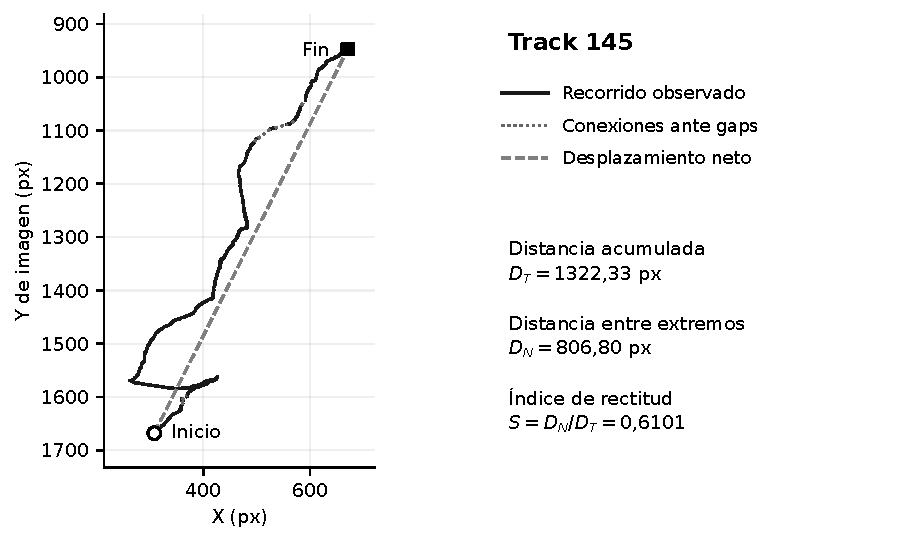
\includegraphics[width=0.90\textwidth]{figures/chapter08/fig08_01_distancias_trayectoria.pdf}
  \caption{Distancia acumulada ($D_T$), distancia entre extremos ($D_N$) y rectitud ($S$) de \texttt{Track\_145}, calculadas sobre sus 929 observaciones. El círculo indica el inicio y el cuadrado, el fin. Los tramos punteados conectan observaciones separadas por gaps y contribuyen a $D_T$ mediante la separación entre sus extremos; la línea discontinua representa $D_N$. Los ejes conservan la misma escala espacial y la orientación vertical de la imagen.}
  \label{fig:distancias-trayectoria}
\end{figure}

\section{Rapidez y suavizado temporal}

\subsection{Rapidez por segmento y promedios}

Para $n\geq2$ observaciones, la rapidez de cada segmento se calcula como
\begin{equation}
  v_i=\frac{\lVert\vec{p}_{i+1}-\vec{p}_i\rVert}{\Delta t_i},
  \qquad \vec{p}_i=(x_i,y_i),\quad i=1,\ldots,n-1.
  \label{eq:rapidez-segmento-implementada}
\end{equation}
El resultado se asocia con el cuadro final $f_{i+1}$. Es una estimación escalar sobre el intervalo entre posiciones observadas, no una medición instantánea de todo el movimiento ocurrido en su interior. Aunque algunas interfaces utilicen la palabra \emph{velocidad}, aquí se emplea \emph{rapidez} para conservar esta distinción.

La inspección individual conserva dos promedios distintos:
\begin{equation}
  \overline{v}_{\mathrm{seg}}=\frac{1}{n-1}\sum_{i=1}^{n-1}v_i,
  \qquad
  \overline{v}_{\mathrm{tray}}=\frac{D_T}{T}
  =\frac{\sum_i v_i\Delta t_i}{\sum_i\Delta t_i}.
  \label{eq:promedios-rapidez}
\end{equation}
El primero asigna el mismo peso a cada segmento; el segundo pondera por su duración. Coinciden cuando los intervalos son iguales, pero pueden diferir ante gaps. Se exponen, respectivamente, como \texttt{mean\_segment\_speed} y \texttt{trajectory\_average\_speed}; el campo de compatibilidad \texttt{avg\_speed} conserva la primera interpretación.

La Figura~\ref{fig:promedios-rapidez} ilustra esa diferencia con tres observaciones en los cuadros $0$, $1$ y $4$, separadas espacialmente por $10$ px en cada segmento. Con $F=30$, se obtienen $300$ y $100$ px/s: su media aritmética es $200$ px/s, mientras que $D_T/T=20/(4/30)=150$ px/s.

\begin{figure}[htbp]
  \centering
  \begin{tikzpicture}[x=1.1cm,y=0.85cm]
    \draw[thesisarrow] (0,0) -- (4.7,0);
    \draw[thesisarrow] (0,0) -- (0,3.7);
    \node[font=\small] at (2.5,-0.85) {Tiempo del video (s)};
    \node[font=\small,rotate=90] at (-0.9,1.9) {Rapidez (px/s)};
    \foreach \y/\v in {1/100,1.5/150,2/200,3/300} {
      \draw (-0.06,\y) -- (0.06,\y);
      \node[font=\small,anchor=east] at (-0.13,\y) {$\v$};
    }
    \foreach \x/\t in {0/0,1/{0{,}033},4/{0{,}133}} {
      \draw (\x,-0.06) -- (\x,0.06);
      \node[font=\small,anchor=north] at (\x,-0.15) {$\t$};
    }
    \draw[dashed] (0,2) -- (4.4,2);
    \draw[densely dotted] (0,1.5) -- (4.4,1.5);
    \fill (1,3) circle (2.5pt);
    \fill (4,1) circle (2.5pt);
    \node[font=\small,anchor=west] at (4.6,3) {Rapidez por segmento};
    \node[font=\small,anchor=west] at (4.6,2) {$\overline{v}_{\mathrm{seg}}=200$ px/s};
    \node[font=\small,anchor=west] at (4.6,1.5) {$\overline{v}_{\mathrm{tray}}=150$ px/s};
  \end{tikzpicture}
  \caption{Ejemplo numérico ilustrativo de los dos promedios de rapidez. Los puntos representan valores por segmento asociados con sus cuadros finales; las líneas horizontales indican promedios. Los tiempos se muestran redondeados. No corresponde a un resultado experimental.}
  \label{fig:promedios-rapidez}
\end{figure}

\subsection{Media móvil y alineación temporal}

La rapidez se suaviza mediante una media móvil de $w$ valores consecutivos de la serie calculada. Si esta contiene $m=n-1$ segmentos, se obtiene
\begin{equation}
  \widetilde{v}_j=\frac{1}{w}\sum_{k=j}^{j+w-1}v_k,
  \qquad j=1,\ldots,m-w+1.
\end{equation}
La operación utiliza únicamente ventanas completas y asigna cada resultado al cuadro del último segmento incluido, $f_{j+w}$. Por tanto, genera $M=m-w+1$ valores cuando $m\geq w$; en caso contrario, devuelve una serie vacía. Con $w=20$ se requieren al menos 21 posiciones para obtener un valor suavizado.

La ventana cuenta muestras, no segundos ni cuadros necesariamente consecutivos. Su duración efectiva puede variar, y la media móvil puede combinar segmentos separados por gaps. El suavizado no divide automáticamente la trayectoria en bloques continuos. También reduce la resolución temporal de variaciones breves y puede desplazar su representación hacia el final de la ventana.

\section{Variación temporal de la rapidez}

Sobre la serie suavizada, el sistema estima diferencias de rapidez por unidad de tiempo. Si $g_j$ es el cuadro asociado con su muestra $j$, el cálculo es
\begin{equation}
  a_j=\frac{\widetilde{v}_{j+1}-\widetilde{v}_j}{(g_{j+1}-g_j)/F}.
  \label{eq:variacion-rapidez-implementada}
\end{equation}
La función utiliza las diferencias reales entre cuadros y requiere al menos dos valores de rapidez. La magnitud se expresa en px/s$^2$ y representa una variación escalar de rapidez. No reconstruye el vector de aceleración ni describe por sí sola cambios de dirección a rapidez constante.

Los gráficos señalan aumentos bruscos si $a_j>A$ y disminuciones bruscas si $a_j<-A$. Estas marcas se asignan a la muestra posterior de la diferencia. El umbral $A$ es operativo; las denominaciones de aceleración o frenada utilizadas en la visualización no establecen un mecanismo físico o biológico.

\section{Inactividad y cambios de régimen}

\subsection{Muestras bajo el umbral de actividad}

La condición de inactividad se aplica a la rapidez suavizada mediante $\widetilde{v}_j<u$. Cuando existen $M>0$ valores, la inspección calcula
\begin{equation}
  I=\frac{1}{M}\sum_{j=1}^{M}\mathbf{1}[\widetilde{v}_j<u].
  \label{eq:fraccion-inactividad}
\end{equation}
El resultado es una fracción entre cero y uno. El campo \texttt{inactivity\_percentage} almacena esa fracción, sin multiplicarla por cien. Sus términos cuentan muestras suavizadas, sin ponderarlas por duración. En consecuencia, no se interpreta directamente como la proporción del tiempo total durante la cual el microorganismo permaneció inmóvil.

La inspección conserva los cuadros finales asociados con las muestras que cumplen el criterio y sus tiempos en el video. El umbral identifica valores reducidos de rapidez según la configuración; no demuestra ausencia de movimiento durante todo el intervalo ni constituye un diagnóstico biológico de inactividad.

\subsection{Comparación entre ventanas de rapidez}

Los cambios de régimen se señalan comparando la media de $r$ muestras suavizadas previas con la de $r$ muestras a partir del punto evaluado. Se marca una posición interior cuando la diferencia absoluta entre esas medias alcanza o supera un umbral $\delta$. El recorrido de la serie excluye los extremos donde la implementación no realiza esa comparación.

El criterio puede marcar varias posiciones cercanas durante una transición, ya que no incorpora una consolidación posterior de eventos. Sus ventanas también se definen por cantidad de muestras y pueden abarcar gaps. Estas marcas describen diferencias entre niveles locales de rapidez; la clasificación del tipo de movimiento se desarrolla en el capítulo siguiente.

El Cuadro~\ref{tab:parametros-analisis-trayectorias} resume los parámetros operativos predeterminados, sin optimización experimental documentada. Las rutinas pueden omitir productos si no hay muestras suficientes para sus ventanas.

\begin{table}[htbp]
  \centering
  \small
  \caption{Parámetros operativos del análisis cuantitativo.}
  \label{tab:parametros-analisis-trayectorias}
  \begin{tabularx}{\textwidth}{@{}l l X@{}}
    \toprule
    Parámetro & Valor & Función \\
    \midrule
    $F$ & $30$ cuadros/s & Frecuencia utilizada para convertir cuadros a tiempo. \\
    $w$ & $20$ muestras & Ventana de la media móvil de rapidez. \\
    $u$ & $30$ px/s & Umbral de inactividad: comparación estricta por debajo. \\
    $A$ & $450$ px/s$^2$ & Umbral de variación brusca de rapidez. \\
    $r$ & $50$ muestras & Tamaño de cada ventana para cambios de régimen. \\
    $\delta$ & $30$ px/s & Diferencia mínima entre medias locales. \\
    \bottomrule
  \end{tabularx}
\end{table}

\section{Resúmenes y visualizaciones}

La inspección individual reúne posiciones, distancias, rapideces y muestras bajo el umbral de actividad. Sus gráficos muestran el recorrido bidimensional, las rapideces originales o suavizadas y las marcas de inactividad o cambio. Los límites del modo \texttt{context} ajustan la ventana visible alrededor de los datos sin reiniciar el origen temporal del video. La trayectoria individual se dibuja con el eje vertical invertido para conservar la orientación de la imagen, sin modificar las coordenadas almacenadas.

En las curvas temporales individuales se insertan interrupciones gráficas ante gaps de la serie y se sombrean sus intervalos. Esto no elimina los segmentos calculados sobre observaciones separadas ni impide que el suavizado abarque esos intervalos. La trayectoria espacial, en cambio, une posiciones consecutivas de la lista, incluso cuando sus cuadros no son consecutivos.

El resumen general ordena trayectorias por distancia acumulada, desviación estándar de las rapideces por segmento e índice de rectitud. La etiqueta de trayectorias más \emph{irregulares} utilizada en la salida se refiere a variabilidad de rapidez, no a irregularidad geométrica. El atributo histórico \texttt{n\_continuous} utiliza rectitud, no cobertura temporal; la corrección de etiquetas lo presenta como ranking de mayor rectitud. Se muestran hasta cinco ejemplos por criterio, según la configuración y la cantidad disponible.

Una función auxiliar permite graficar la media de rapideces agrupadas por el cuadro final de cada segmento. Ese promedio reúne solo los tracks con una rapidez asociada al cuadro correspondiente; no presupone un conjunto constante de individuos ni equivale a una media de trayectorias completas. Su disponibilidad se distingue de los productos activados por defecto en el procesamiento general.

\begin{samepage}
El ejemplo geométrico de la Figura~\ref{fig:distancias-trayectoria} ilustra la construcción y el significado de las distancias y la rectitud. La evaluación experimental y las comparaciones con referencias manuales se desarrollan en el capítulo~\ref{chap:evaluacion-resultados}.
\par
\end{samepage}

\section{Consideraciones y limitaciones}

Las métricas dependen de las posiciones, la identidad asignada por el seguimiento y los FPS de análisis. Una frecuencia incorrecta modifica la escala temporal de la rapidez y de sus variaciones. Los errores de localización pueden introducir fluctuaciones; los cambios de identidad pueden generar segmentos que mezclen individuos. El suavizado y los umbrales no garantizan la corrección de esos casos.

Los gaps se conservan en los intervalos temporales, pero no permiten conocer el recorrido intermedio. Las ventanas móviles y los promedios sin ponderación temporal deben interpretarse considerando esa disponibilidad desigual. Tampoco se equipara una rectitud elevada con seguimiento correcto o con una categoría de movimiento específica.

\begin{samepage}
Los valores no definidos y las series vacías deben distinguirse de resultados físicamente nulos. Algunas salidas de compatibilidad muestran cero cuando faltan rapideces; ese valor no demuestra estacionariedad. Asimismo, una trayectoria con pocos puntos puede devolver distancia acumulada nula sin contener observaciones suficientes para caracterizar el movimiento.
\par
\end{samepage}

En la revisión utilizada para reconstruir los resultados, la referencia relativa de la curva no se aplicaba a las marcas auxiliares de inicio, fin y gaps. La corrección de presentación utiliza los cuadros originales de las posiciones para incluir el gap inicial y expresa también las marcas auxiliares en la referencia elegida. Esa modificación conserva las muestras y los cálculos numéricos. La descripción principal de este capítulo utiliza el tiempo del video, que es la referencia predeterminada de los gráficos.

En la versión corregida de las visualizaciones operativas, las gráficas espaciales y las estelas de los videos individuales se interrumpen ante cuadros ausentes. Las conexiones punteadas del ejemplo geométrico de la Figura~\ref{fig:distancias-trayectoria} conservan un propósito distinto: ilustran la separación entre extremos que contribuye a la distancia acumulada, sin afirmar un recorrido observado durante el gap.

\chapter[Clasificación de patrones de movimiento]{Clasificación de patrones\\de movimiento}
\label{chap:clasificacion-movimiento}

El sistema desarrollado asigna una categoría a cada trayectoria mediante puntuaciones construidas a partir de sus características geométricas. Este capítulo especifica las métricas adicionales, las fórmulas de combinación y las reglas de decisión del clasificador. Las categorías se utilizan con el alcance descriptivo establecido en el capítulo 3; la evaluación sobre los videos experimentales se reserva para el capítulo de resultados.

\section{Entrada y alcance de la clasificación}

El clasificador recibe las observaciones ordenadas $(f_i,x_i,y_i)$ de una trayectoria, con la representación definida en los capítulos anteriores. Verifica que los índices de cuadro sean estrictamente crecientes y que la frecuencia de análisis sea positiva. La decisión se aplica al recorrido completo: no se divide la trayectoria en etapas ni se asignan categorías distintas a sus intervalos.

La clasificación es una etapa opcional del procesamiento general y se encuentra desactivada por defecto. Cuando se habilita, opera sobre las trayectorias que conserva el filtro seleccionado en el capítulo~\ref{chap:seguimiento}. La integración omite aquellas con menos de dos observaciones; las restantes pueden recibir una categoría o un estado de clasificación. El mínimo de puntos exigido por el clasificador es una condición adicional, independiente de ese filtrado previo.

Se calculan tres puntuaciones: direccional, errática y circular u oscilatoria. No se entrena un modelo con trayectorias etiquetadas para obtenerlas. Las reglas y sus parámetros están fijados en la implementación, mientras que los estados \textit{datos insuficientes} y \textit{desconocido} cubren condiciones específicas en las que no se asigna una de las tres categorías.

\section{Características utilizadas}

Se reutilizan la distancia acumulada $D_T$, la distancia neta $D_N$ y el índice de rectitud $S$ descritos en el capítulo~\ref{chap:analisis-trayectorias}. El campo denominado tortuosidad se define aquí como $1-S$, cuando $D_T>0$. Esta elección corresponde al indicador concreto empleado por el clasificador.

\subsection{Orientaciones y cambios angulares}

Para cada desplazamiento entre posiciones registradas se calcula su orientación mediante la función $\operatorname{atan2}$. Se excluyen los vectores cuya norma no supera $10^{-8}$ px, porque no proporcionan una orientación utilizable. Sean $\theta_1,\ldots,\theta_q$ las orientaciones restantes y $m=\max(q-1,0)$. Los cambios entre orientaciones sucesivas se expresan como
\begin{equation}
  \phi_j=\operatorname{atan2}\bigl(\sin(\theta_{j+1}-\theta_j),
                                    \cos(\theta_{j+1}-\theta_j)\bigr),
  \qquad j=1,\ldots,m.
\end{equation}
La expresión conserva el cambio angular principal y evita que el paso entre $-\pi$ y $\pi$ se interprete como un giro cercano a una vuelta completa. Al excluir desplazamientos casi nulos, las orientaciones comparadas pueden corresponder a segmentos que no eran adyacentes en la lista original.

Sobre estos cambios se obtienen la media de sus magnitudes $\mu_{|\phi|}$, la desviación estándar de sus magnitudes $\sigma_{|\phi|}$ y la desviación estándar de los valores con signo $\sigma_\phi$. Las dos desviaciones son diferentes: una describe la dispersión de la magnitud de los giros y la otra también refleja la alternancia de su sentido. Se utilizan desviaciones poblacionales, con divisor $m$.

El número $K$ de cambios de dirección cuenta los casos con $|\phi_j|>\alpha$, donde $\alpha$ es un umbral en radianes. Su proporción se expresa como $U=K/m$ cuando existen cambios angulares. Si no se obtiene ninguno, la implementación asigna cero a las estadísticas angulares y a esa proporción. Los ángulos se calculan entre los desplazamientos disponibles, incluidos los que atraviesan gaps; no se reconstruyen orientaciones dentro de esos intervalos.

\subsection{Proximidad y distribución espacial}

El indicador denominado \textit{tasa de retorno} utiliza un radio proporcional a la diagonal de la caja que contiene las posiciones. Si esa diagonal es $L$ y la fracción configurada es $\rho$, el radio es $r=\rho L$. Para las posiciones $\mathbf p_i=(x_i,y_i)$, el indicador se calcula como
\begin{equation}
 R=\frac{1}{n}\sum_{i=1}^{n}
 \mathbf{1}\!\left[\exists j:\ 0<\|\mathbf p_i-\mathbf p_j\|<r\right].
\end{equation}
Por tanto, mide la fracción de posiciones que tienen alguna otra posición a distancia positiva e inferior a $r$. No exige que esta sea posterior, no impone una separación temporal mínima y excluye coincidencias espaciales exactas. Incluso posiciones consecutivas de un recorrido rectilíneo pueden contribuir. Su nombre en la salida no debe interpretarse como un conteo de retornos temporales. Si $L<10^{-8}$ px, devuelve cero.

La dispersión radial se obtiene respecto del centroide $\bar{\mathbf p}$. Si $r_i=\|\mathbf p_i-\bar{\mathbf p}\|$, se calcula el coeficiente $C_r=\operatorname{std}(r_i)/\operatorname{mean}(r_i)$. Una dispersión baja indica distancias similares al centroide, aunque por sí sola no demuestra un recorrido circular. Si la media radial es inferior a $10^{-8}$ px, el indicador devuelve cero.

La cobertura angular $A$ utiliza los ángulos polares de las posiciones respecto del mismo centroide. Se ordenan y se determina el mayor intervalo angular vacío $G_{\max}$, incluido el que cierra la vuelta. Se calcula $A=1-G_{\max}/(2\pi)$. Esta cobertura describe la distribución espacial de los ángulos: no utiliza el orden de visita ni mide el número de vueltas realizadas.

\subsection{Características complementarias}

La salida incluye también el número de inversiones del desplazamiento proyectado sobre el primer eje principal de las posiciones. Ese eje se obtiene mediante descomposición en valores singulares. Se excluyen los incrementos cuya magnitud no supera el 1\% de la máxima proyección absoluta respecto del centroide y se cuentan los cambios de signo entre los restantes.

Además, se informa el coeficiente de variación de las rapideces por segmento, calculadas con los intervalos reales entre cuadros y la frecuencia de análisis del capítulo~\ref{chap:analisis-trayectorias}. No se utiliza la serie suavizada. Si la rapidez media es inferior a $10^{-8}$ px/s, el coeficiente devuelve cero.

Estas dos características se conservan para inspección, pero no intervienen en las puntuaciones actuales. En particular, el número de inversiones no participa en la categoría denominada circular u oscilatoria. Los valores cero usados en casos degenerados son convenciones de cálculo y requieren distinguirse de evidencia de regularidad del movimiento.

\section{Construcción de las puntuaciones}

Los indicadores se combinan mediante medias de términos limitados al intervalo $[0,1]$. Se define $C(z)=\max(0,\min(1,z))$ y se introducen las cantidades
\begin{equation}
\begin{aligned}
 a&=C(\mu_{|\phi|}/\pi), & b&=C(\sigma_{|\phi|}/\pi),
 &u&=C(U),\\
 r_s&=C(R), & g&=C(A), &h&=C(C_r),\\
 z&=C(\sigma_\phi/\pi).
\end{aligned}
\end{equation}
El subíndice de $r_s$ distingue la proximidad normalizada del radio espacial $r$. Las tres puntuaciones son
\begin{equation}
\begin{aligned}
 Q_D&=\frac{S+(1-a)+(1-b)+(1-r_s)}{4},\\[0.3em]
 Q_E&=\frac{(1-S)+a+b+u}{4},\\[0.3em]
 Q_C&=\frac{(1-S)+g+(1-h)+(1-u)+(1-z)}{5}.
\end{aligned}
\label{eq:puntuaciones-movimiento}
\end{equation}

La puntuación direccional favorece una rectitud alta, giros de poca magnitud y dispersión, y un valor reducido de proximidad espacial. La errática favorece baja rectitud, mayor magnitud y dispersión de los giros, y una mayor proporción de cambios por encima del umbral angular. La circular u oscilatoria combina baja rectitud, cobertura angular alta, baja dispersión radial, pocos cambios por encima del umbral y baja dispersión de los giros con signo.

Cada término tiene el mismo peso dentro de su puntuación, aunque las categorías utilizan distinto número de términos. Los valores no se normalizan para sumar uno y no constituyen probabilidades. Tampoco se establece una correspondencia exclusiva entre una característica y un patrón: diferentes geometrías pueden producir puntuaciones próximas o favorecer una misma categoría.

Las distancias, los índices y las estadísticas angulares se redondean a cuatro decimales antes de combinarse. La clasificación utiliza las puntuaciones calculadas a partir de esas métricas y redondea a cuatro decimales los valores que entrega en la salida.

\section{Regla de decisión y parámetros}

Primero se compara la cantidad de posiciones con el mínimo $n_{\min}$. Si no se alcanza, se devuelve el estado \textit{datos insuficientes}, con puntuaciones y confianza iguales a cero; en ese caso solo se informa la cantidad de puntos. Esta regla no comprueba la cobertura temporal ni la representatividad del recorrido.

Si se cumple el mínimo, se calculan las métricas. Cuando la distancia acumulada redondeada es inferior a $10^{-4}$ px, se devuelve \textit{desconocido}, con puntuaciones y confianza iguales a cero. Esta condición impide evaluar las expresiones que requieren rectitud definida. No equivale al criterio de inactividad del capítulo~\ref{chap:analisis-trayectorias}.

En los demás casos se selecciona la categoría cuya puntuación es máxima. Si el máximo es inferior al umbral $\gamma$, el resultado se sustituye por \textit{desconocido}, conservando las puntuaciones calculadas. No se exige una diferencia mínima entre las dos puntuaciones más altas. En un empate exacto se conserva el orden de evaluación: direccional, errática y circular u oscilatoria.

\begin{table}[htbp]
 \centering
 \caption{Parámetros predeterminados del clasificador.}
 \label{tab:parametros-clasificacion}
 \begin{tabularx}{\textwidth}{@{}l l X@{}}
  \toprule
  Parámetro & Valor & Función \\
  \midrule
  $n_{\min}$ & 15 posiciones & Mínimo exigido para calcular la clasificación. \\
  $\rho$ & 0,10 & Fracción de la diagonal de la caja para el radio de proximidad. \\
  $\alpha$ & 0,5 rad & Umbral estricto para contar cambios de dirección. \\
  $\gamma$ & 0,35 & Mínimo de la puntuación máxima para aceptar una categoría. \\
  \bottomrule
 \end{tabularx}
\end{table}

El umbral predeterminado tiene una limitación derivada de las fórmulas. Al sumar las puntuaciones direccional y errática se obtiene
\begin{equation}
 Q_D+Q_E=1+\frac{u-r_s}{4}\geq 0{,}75.
\end{equation}
Por tanto, al menos una alcanza $0{,}375$, por encima de $\gamma=0{,}35$. El redondeo de las métricas no modifica esta conclusión. En la configuración actual, la comparación con ese umbral no rechaza las trayectorias que llegan al cálculo de puntuaciones; el estado \textit{desconocido} queda reservado, en la práctica, a la condición previa sobre la distancia. Modificar $\gamma$ puede activar el rechazo por puntuación, pero no incorpora una medida de separación entre categorías.

La Figura~\ref{fig:decision-clasificacion} resume el procedimiento. Los parámetros del Cuadro~\ref{tab:parametros-clasificacion} son decisiones operativas de la implementación; su validación sobre las trayectorias experimentales requiere una evaluación específica.

\begin{figure}[H]
 \centering
 \begin{tikzpicture}[node distance=6mm,
  box/.style={thesisflow,text width=5.9cm},
  side/.style={thesisflow,text width=3.2cm},
  ]
  \node[box] (input) {Trayectoria con orden temporal válido};
  \node[box,below=of input] (minimum) {¿Alcanza $n_{\min}$ posiciones?};
  \node[side,right=9mm of minimum] (short) {Datos insuficientes};
  \node[box,below=of minimum] (distance) {Calcular métricas\\¿Distancia redondeada $\geq 10^{-4}$ px?};
  \node[side,right=9mm of distance] (zero) {Desconocido};
  \node[box,below=of distance] (scores) {Calcular $Q_D$, $Q_E$, $Q_C$\\y seleccionar el máximo};
  \node[box,below=of scores] (floor) {¿El máximo alcanza $\gamma$?};
  \node[side,right=9mm of floor] (reject) {Desconocido};
  \node[box,below=of floor] (output) {Categoría seleccionada, puntuaciones\\y métricas};
  \draw[thesisarrow] (input) -- (minimum);
  \draw[thesisarrow] (minimum) -- node[right,font=\small] {Sí} (distance);
  \draw[thesisarrow] (minimum) -- node[above,font=\small] {No} (short);
  \draw[thesisarrow] (distance) -- node[right,font=\small] {Sí} (scores);
  \draw[thesisarrow] (distance) -- node[above,font=\small] {No} (zero);
  \draw[thesisarrow] (scores) -- (floor);
  \draw[thesisarrow] (floor) -- node[right,font=\small] {Sí} (output);
  \draw[thesisarrow] (floor) -- node[above,font=\small] {No} (reject);
 \end{tikzpicture}
 \caption{Reglas de decisión del clasificador. La rama de rechazo por $\gamma$ se conserva como parte del algoritmo configurable, con la limitación indicada para su valor predeterminado.}
 \label{fig:decision-clasificacion}
\end{figure}

\section{Información generada e inspección}

Cada resultado identifica la categoría o el estado mediante el campo \texttt{movement\_type}. Los identificadores de las categorías son \texttt{directional}, \texttt{brownian\_erratic} y \texttt{circular\_oscillatory}; los estados adicionales son \texttt{insufficient\_data} y \texttt{unknown}. La denominación errática describe características geométricas y no acredita un mecanismo físico browniano.

El campo \texttt{scores} conserva las tres puntuaciones y \texttt{metrics} reúne las características disponibles. El campo \texttt{confidence} contiene la puntuación máxima, salvo los casos previos al cálculo de puntuaciones, en los que vale cero. Se interpreta como el valor de la regla ganadora y no como una probabilidad calibrada de acierto. Su comparación entre trayectorias tampoco incorpora la diferencia respecto de la segunda puntuación.

La explicación de \texttt{reason} procede de un texto fijo asociado con la categoría o el estado. No se genera examinando qué términos dominaron en cada trayectoria. En particular, el texto de la categoría circular u oscilatoria menciona retornos frecuentes, aunque $R$ no aparece en $Q_C$. Para inspeccionar una asignación deben consultarse las métricas y las fórmulas, además de esa explicación general.

Cuando la etapa está habilitada, el procesamiento informa la cantidad de trayectorias por categoría o estado y muestra hasta cinco resultados ordenados por el campo de confianza. El guardado en JSON es una opción adicional, también desactivada por defecto, y se realiza dentro de la etapa de clasificación. El archivo agrupa los resultados por identificador de trayectoria. Las opciones de activación se registran en los metadatos de ejecución; los cuatro parámetros propios del clasificador no se incorporan allí explícitamente en la integración actual.

La Figura~\ref{fig:ejemplos-clasificacion} compara tres recorridos sintéticos de 41 observaciones en cuadros consecutivos, con los parámetros predeterminados. El rectilíneo usa incrementos uniformes y el circular, una vuelta con pasos angulares uniformes. El irregular acumula incrementos normales estándar bidimensionales generados con \texttt{default\_rng} de NumPy y semilla 4.

\begin{figure}[H]
 \centering
 \begin{tikzpicture}[x=1cm,y=1cm]
  \begin{scope}[xshift=0.0cm]
   \node[font=\small\bfseries] at (2.2,3.65) {Recorrido rectilíneo};
   \draw[line width=0.65pt,-{Latex[length=1.5mm]}] plot coordinates {(0.3000,2.0500) (0.3950,2.0500) (0.4900,2.0500) (0.5850,2.0500) (0.6800,2.0500) (0.7750,2.0500) (0.8700,2.0500) (0.9650,2.0500) (1.0600,2.0500) (1.1550,2.0500) (1.2500,2.0500) (1.3450,2.0500) (1.4400,2.0500) (1.5350,2.0500) (1.6300,2.0500) (1.7250,2.0500) (1.8200,2.0500) (1.9150,2.0500) (2.0100,2.0500) (2.1050,2.0500) (2.2000,2.0500) (2.2950,2.0500) (2.3900,2.0500) (2.4850,2.0500) (2.5800,2.0500) (2.6750,2.0500) (2.7700,2.0500) (2.8650,2.0500) (2.9600,2.0500) (3.0550,2.0500) (3.1500,2.0500) (3.2450,2.0500) (3.3400,2.0500) (3.4350,2.0500) (3.5300,2.0500) (3.6250,2.0500) (3.7200,2.0500) (3.8150,2.0500) (3.9100,2.0500) (4.0050,2.0500) (4.1000,2.0500)};
   \fill (0.3000,2.0500) circle[radius=1pt];
   \node[font=\small,align=center] at (2.2,-0.25) {$Q_D=0,7500$\\$Q_E=0,0000$\\$Q_C=0,5844$};
  \end{scope}
  \begin{scope}[xshift=5.1cm]
   \node[font=\small\bfseries] at (2.2,3.65) {Recorrido irregular};
   \draw[line width=0.65pt,-{Latex[length=1.5mm]}] plot coordinates {(3.5373,0.9563) (4.1000,1.1792) (3.5449,1.1775) (3.3340,1.2277) (2.7901,1.3095) (2.8697,1.8424) (2.9768,2.0151) (2.4718,2.7769) (1.8240,3.1496) (1.7124,2.8517) (1.4904,2.6245) (1.6190,2.5872) (2.1204,1.9685) (2.1194,1.6668) (2.3818,0.9504) (2.2655,1.0215) (1.7636,1.3547) (1.8240,1.6952) (2.1484,1.3638) (1.8786,1.2951) (2.1316,1.5829) (1.8915,1.3775) (1.6217,1.1799) (1.5412,1.1353) (2.2373,0.9641) (2.1397,1.1192) (1.8173,0.9945) (1.8218,1.2563) (1.3767,1.7202) (1.2575,1.7775) (1.5440,2.0009) (1.9023,2.0595) (1.8956,2.1665) (1.5589,2.5772) (1.2966,2.1510) (1.9921,2.1048) (1.5933,2.7313) (1.4818,3.0905) (1.2013,3.0063) (0.6302,2.3607) (0.3000,2.3343)};
   \fill (3.5373,0.9563) circle[radius=1pt];
   \node[font=\small,align=center] at (2.2,-0.25) {$Q_D=0,3976$\\$Q_E=0,5502$\\$Q_C=0,5885$};
  \end{scope}
  \begin{scope}[xshift=10.2cm]
   \node[font=\small\bfseries] at (2.2,3.65) {Recorrido circular};
   \draw[line width=0.65pt,-{Latex[length=1.5mm]}] plot coordinates {(3.3750,2.0500) (3.3605,2.2338) (3.3175,2.4131) (3.2469,2.5834) (3.1506,2.7406) (3.0309,2.8809) (2.8906,3.0006) (2.7334,3.0969) (2.5631,3.1675) (2.3838,3.2105) (2.2000,3.2250) (2.0162,3.2105) (1.8369,3.1675) (1.6666,3.0969) (1.5094,3.0006) (1.3691,2.8809) (1.2494,2.7406) (1.1531,2.5834) (1.0825,2.4131) (1.0395,2.2338) (1.0250,2.0500) (1.0395,1.8662) (1.0825,1.6869) (1.1531,1.5166) (1.2494,1.3594) (1.3691,1.2191) (1.5094,1.0994) (1.6666,1.0031) (1.8369,0.9325) (2.0162,0.8895) (2.2000,0.8750) (2.3838,0.8895) (2.5631,0.9325) (2.7334,1.0031) (2.8906,1.0994) (3.0309,1.2191) (3.1506,1.3594) (3.2469,1.5166) (3.3175,1.6869) (3.3605,1.8662) (3.3750,2.0500)};
   \fill (3.3750,2.0500) circle[radius=1pt];
   \node[font=\small,align=center] at (2.2,-0.25) {$Q_D=0,4875$\\$Q_E=0,2625$\\$Q_C=0,9914$};
  \end{scope}
 \end{tikzpicture}
 \caption{Recorridos sintéticos y puntuaciones obtenidas con la implementación actual. El punto marca el inicio y la flecha indica el final. Los paneles conservan la proporción espacial de cada recorrido, con escalas independientes. Son ejemplos de cálculo, no resultados experimentales.}
 \label{fig:ejemplos-clasificacion}
\end{figure}

En el recorrido irregular, la puntuación circular supera a la errática. El ejemplo permite verificar cómo compiten las reglas y por qué la forma visual de una trayectoria no garantiza una etiqueta determinada. No constituye una estimación del desempeño sobre los videos ni una validación de los umbrales.

\section{Alcance y limitaciones del método}

Las reglas resumen propiedades de las posiciones disponibles. Los gaps no activan una división automática en tramos ni reducen directamente la puntuación: pueden producirse giros entre segmentos separados temporalmente y proximidades entre posiciones distantes en el tiempo. El filtro previo permite seleccionar trayectorias, pero el clasificador no incorpora una evaluación propia de cobertura o duración mínima.

La densidad de muestreo modifica la proximidad espacial, la distribución de giros y los conteos de cambios e inversiones. Por ello, obtener suficientes puntos no garantiza que dos trayectorias representen duraciones o resoluciones comparables. La distancia acumulada y la rapidez siguen dependiendo de las limitaciones descritas en el capítulo~\ref{chap:analisis-trayectorias}. La proximidad utiliza comparaciones entre todos los pares de posiciones, con un costo cuadrático respecto de su cantidad.

La categoría circular u oscilatoria reúne comportamientos distintos mediante una sola puntuación. Aunque se informa el número de inversiones sobre el eje principal, este no interviene en la decisión. La clasificación global tampoco localiza transiciones entre patrones dentro de una trayectoria. Estas restricciones deben considerarse al contrastar sus resultados con una revisión manual.

Las puntuaciones, sus pesos y los umbrales requieren validación con casos representativos y criterios de referencia. El sistema entrega una descripción computacional inspeccionable; atribuir un mecanismo físico o biológico al recorrido exige evidencia adicional. Las pruebas de implementación se documentan en el capítulo siguiente y la evaluación experimental se presenta posteriormente.

\chapter{Implementación y pruebas del sistema}
\label{chap:implementacion-pruebas}

Este capítulo documenta la ejecución del sistema desarrollado, su trazabilidad y las pruebas de sus cálculos e integración. Se apoya en la arquitectura del capítulo 5 y los métodos de los capítulos 6 a 9. La evaluación con videos experimentales corresponde al capítulo 11.

\section{Entorno de implementación y dependencias}

La implementación utiliza Python 3.12 y bibliotecas especializadas para inferencia, procesamiento de video, cálculo numérico y visualización. El Cuadro~\ref{tab:entorno-implementacion} reúne las dependencias principales del entorno de referencia en CPU. Las versiones se fijan en archivos de dependencias para reducir las variaciones introducidas por actualizaciones del software.

\begin{table}[htbp]
 \centering
 \caption{Dependencias principales del entorno de referencia.}
 \label{tab:entorno-implementacion}
 \small
 \begin{tabularx}{\textwidth}{@{}l l X@{}}
  \toprule
  Componente & Versión & Función \\
  \midrule
  Python & 3.12.x & Ejecución del sistema. \\
  NumPy & 2.2.6 & Operaciones numéricas sobre posiciones y series. \\
  Matplotlib & 3.10.8 & Generación de gráficos. \\
  OpenCV & 4.11.0.86 & Lectura y escritura de video. \\
  PyTorch / Torchvision & 2.7.1 / 0.22.1 (CPU) & Soporte de inferencia. \\
  Ultralytics & 8.3.213 & Detección y seguimiento. \\
  pytest & 9.1.1 & Ejecución de pruebas automatizadas. \\
  \bottomrule
 \end{tabularx}
\end{table}

Colab utiliza un perfil separado, con el PyTorch y el acelerador disponibles en ese servicio. La GPU NVIDIA T4 del entrenamiento descrito en el capítulo 6 no es un requisito de toda ejecución posterior.

Una utilidad comprueba Python, dependencias y, opcionalmente, existencia y extensiones de las entradas externas. No certifica el contenido del video, la adecuación de los pesos ni la validez de las anotaciones.

\section{Integración y ejecución del procesamiento}

El procesamiento general se invoca desde Python mediante la función \texttt{process\_video\_general}. Recibe las rutas del video y los pesos, el directorio de salida y las opciones de análisis. Las entradas se conservan fuera del código: utilizar otro video o modelo no requiere modificar las funciones de cálculo.

La función coordina el seguimiento, el filtrado y los productos solicitados. Devuelve el diccionario de trayectorias, incluso al habilitar la clasificación o los gráficos. Las interfaces de inspección reutilizan ese diccionario para consultar métricas y generar productos individuales sin repetir la inferencia.

Activar la clasificación no obliga a guardarla, y solicitar su guardado sin habilitarla no produce el archivo. El video anotado de Ultralytics utiliza el destino de esa biblioteca, independiente del directorio general de salida. Las pruebas de integración y de salidas comprueban estas condiciones y la propagación de parámetros.

\section{Validación de entradas y tratamiento de errores}

El punto de entrada rechaza una frecuencia de análisis no positiva y los modos de eje temporal no admitidos. La selección de trayectorias también rechaza nombres de filtro desconocidos. Las funciones que requieren intervalos temporales comprueban el orden de las observaciones antes de operar: cuadros repetidos o decrecientes producen una excepción. Los gaps válidos conservan sus índices originales, de acuerdo con el capítulo~\ref{chap:seguimiento}.

Se distinguen tres situaciones. Un valor cero representa una magnitud calculable cuyo resultado es nulo; \texttt{None} representa una magnitud no definida o no calculable; una excepción señala que la entrada incumple una condición requerida. Por ejemplo, una trayectoria estacionaria puede tener rapidez cero y rectitud no definida. Una trayectoria de una sola observación no aporta segmentos para calcular rapidez y las funciones correspondientes devuelven series vacías. El tratamiento concreto depende de la operación solicitada.

Las comprobaciones se aplican en los componentes que consumen los datos, sin validación exhaustiva anticipada. Los errores de seguimiento o escritura que se propagan interrumpen el procesamiento. Pueden quedar productos parciales; no se garantiza un informe de error persistente ni la eliminación de archivos anteriores.

\section{Trazabilidad y reproducibilidad}

Al completar el flujo, se escribe \texttt{run\_metadata.json}. El archivo registra las rutas del video y del modelo, los umbrales de detección, los FPS de análisis, los parámetros analíticos, el filtro y las opciones activadas. También incluye fecha, plataforma, versión de Python y versiones de las bibliotecas principales. Cuando la información está disponible, registra la revisión del código y si existen cambios locales; los campos que no pueden recuperarse permanecen nulos.

Los metadatos no contienen las trayectorias ni las series calculadas. Las marcas de salida indican productos solicitados, sin comprobar todos los archivos generados. El estado de éxito indica que el flujo llegó a escribir los metadatos; no certifica la calidad científica de los resultados.

El registro no calcula huellas de los pesos y del video: sus rutas no verifican la identidad del contenido. Tampoco conserva todos los parámetros del clasificador ni el estado completo del acelerador. Repetir un análisis exige conservar entradas, configuración y versión de implementación. El entorno fijado facilita esa tarea, sin garantizar resultados idénticos entre plataformas o dispositivos.

\section{Estrategia de pruebas automatizadas}

Las pruebas numéricas comparan resultados con valores deducidos independientemente para entradas sencillas. Las de contratos comprueban interfaces, valores predeterminados, retornos y errores esperados. Las de regresión conservan comportamientos establecidos, sin demostrar su adecuación para cualquier situación experimental.

Las pruebas de integración verifican la coordinación entre seguimiento, selección, análisis, clasificación y metadatos. Para ejecutarlas sin pesos ni videos reales se sustituyen componentes por versiones deterministas: el seguimiento entrega trayectorias conocidas y algunas pruebas reemplazan las funciones gráficas por funciones que registran sus llamadas. Otras pruebas examinan la creación efectiva de archivos y las propiedades de las visualizaciones. La sustitución permite aislar errores de integración, pero deja fuera el desempeño real de la inferencia.

La suite incluye además comprobaciones de normalización de anotaciones, cálculo de errores frente a referencias, inventario del conjunto piloto y organización de artefactos. Esas pruebas verifican la infraestructura de evaluación sobre casos controlados; no equivalen a evaluar el sistema con una referencia manual experimental. El Cuadro~\ref{tab:matriz-pruebas} resume casos representativos sin reproducir el inventario completo de archivos.

\begin{table}[htbp]
 \centering
 \caption{Casos representativos de verificación del sistema.}
 \label{tab:matriz-pruebas}
 \footnotesize
 \renewcommand{\arraystretch}{1.12}
 \begin{tabularx}{\textwidth}{@{}p{0.22\textwidth}X X@{}}
  \toprule
  Comportamiento & Entrada controlada & Resultado esperado \\
  \midrule
  Distancias & Dos segmentos perpendiculares de 3 y 4 px. & Distancia acumulada de 7 px y neta de 5 px. \\
  Rapidez con gaps & Desplazamientos e intervalos temporales conocidos. & División por el tiempo real entre observaciones. \\
  Orden temporal & Cuadros repetidos o decrecientes. & Rechazo mediante \texttt{ValueError}. \\
  Casos degenerados & Una observación o posiciones estacionarias. & Series vacías, ceros o magnitudes no definidas según la operación. \\
  Clasificación & Recorridos sintéticos y cantidades de puntos conocidas. & Categorías o estados coherentes con las reglas implementadas. \\
  Integración & Trayectorias deterministas y opciones de procesamiento. & Selección, llamadas, retornos y guardado según la configuración. \\
  Referencias & Predicciones idénticas, desplazadas o incompletas. & Errores y cobertura acordes con el caso construido. \\
  Metadatos & Configuraciones y entornos controlados. & Persistencia de los valores efectivos y campos nulos previstos. \\
  \bottomrule
 \end{tabularx}
\end{table}

\section{Prueba controlada de rapidez con observaciones ausentes}

Para ilustrar una comprobación numérica se utiliza una trayectoria sintética con observaciones en los cuadros 0, 1, 4 y 5. Las posiciones horizontales son 0, 2, 8 y 10 px, respectivamente, y la coordenada vertical es cero. Se fija una frecuencia de análisis de 30 FPS. Los cuadros 2 y 3 no tienen observaciones; no se incorporan posiciones interpoladas.

El resultado esperado es 60 px/s en cada uno de los tres segmentos. En el intervalo que atraviesa el gap, el desplazamiento es de 6 px y el tiempo transcurrido es de $3/30$ s. Por tanto, aplicar la definición del capítulo~\ref{chap:analisis-trayectorias} conserva el mismo valor que en los segmentos de cuadros consecutivos. La prueba detectaría un cálculo que tratara todas las observaciones como consecutivas, porque ese procedimiento alteraría la rapidez del segmento central.

La Figura~\ref{fig:prueba-rapidez-gaps} muestra las entradas y los valores obtenidos al ejecutar la función real de cálculo. La comparación numérica utiliza tolerancias absoluta y relativa de $10^{-12}$; en este caso, los tres errores absolutos son cero. También se comprueba que los valores quedan asociados a los cuadros finales 1, 4 y 5.

\begin{figure}[htbp]
 \centering
 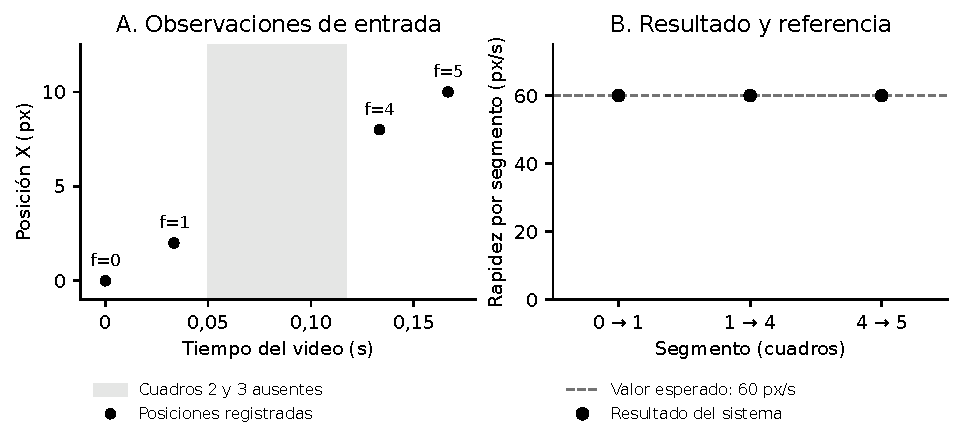
\includegraphics[width=\textwidth]{figures/chapter10/fig10_01_prueba_rapidez_gaps.pdf}
 \caption{Prueba sintética de rapidez con observaciones ausentes. A: posiciones registradas y franja correspondiente a los cuadros 2 y 3 sin observación. B: rapidez calculada para cada segmento y valor esperado. Los resultados coinciden en 60 px/s; cada punto representa una rapidez media entre dos posiciones, no una medición instantánea dentro del intervalo.}
 \label{fig:prueba-rapidez-gaps}
\end{figure}

Un script importa la función del sistema y guarda el gráfico y un registro JSON de entradas, resultados, tolerancias, versiones y huellas de los archivos fuente. La prueba aísla el cálculo de rapidez sin ejecutar el detector; no valida la localización ni reconstruye lo ocurrido dentro del gap.

\section{Alcance de la verificación}

La ejecución de la suite sobre la revisión \texttt{cf1db739a9e2} del sistema finalizó con 381 pruebas aprobadas, sin pruebas omitidas. Se utilizó Linux con Python 3.12.14, NumPy 2.2.6, Matplotlib 3.10.8, OpenCV 4.11.0.86 y pytest 9.1.1. Esta ejecución empleó la sustitución de la interfaz de YOLO prevista en la configuración de pruebas y no instaló PyTorch, Torchvision ni Ultralytics. Por ello, no corresponde a una comprobación del entorno completo de inferencia del Cuadro~\ref{tab:entorno-implementacion}. La prueba ilustrada se ejecutó adicionalmente sobre esa misma revisión.

Los resultados aportan evidencia de consistencia numérica y de integración para los casos cubiertos. No acreditan la exactitud del detector, la conservación de identidad en cruces u oclusiones, la adecuación de los umbrales ni la validez física de las categorías de movimiento. Tampoco establecen tiempos de procesamiento sobre videos reales. Esos aspectos requieren la evaluación experimental del capítulo 11 y deben distinguirse de la aprobación de las pruebas automatizadas.

\chapter{Evaluación experimental y resultados}
\label{chap:evaluacion-resultados}

Este capítulo presenta los resultados obtenidos con los datos experimentales conservados. Se distinguen las métricas registradas durante el entrenamiento del detector, la comparación de una trayectoria automática con anotaciones manuales y el análisis posterior de sus magnitudes de movimiento. Las pruebas controladas del capítulo~\ref{chap:implementacion-pruebas} verifican operaciones e integración; aquí se examina qué información aportan los datos reales y hasta dónde permiten evaluar el sistema desarrollado.

La evidencia cuantitativa de seguimiento se concentra en una trayectoria de referencia parcial. Por tanto, los resultados describen un caso experimental y no una estimación del desempeño sobre todos los microorganismos del video. La reconstrucción posterior de métricas y categorías se identifica como tal para distinguirla de los productos generados durante la ejecución original.

\section{Material experimental y configuración de la prueba}

La prueba analizada corresponde a \texttt{primer\_minuto.mp4}, un video de $1080\times2336$ píxeles, 30 cuadros por segundo y 1800 cuadros, equivalentes a 60 s de imagen. El archivo \texttt{run\_metadata.json} identifica este video y los pesos del modelo adaptado con la versión 1 del dataset. Las versiones y la preparación de los conjuntos de imágenes se describieron en el capítulo~\ref{chap:deteccion}.

El Cuadro~\ref{tab:configuracion-experimental} reúne la configuración conservada. Los umbrales de detección efectivos difieren de los valores predeterminados de la aplicación: la prueba utilizó $0{,}4$ tanto para confianza como para IoU de NMS. Este último parámetro no constituye un umbral de evaluación del seguimiento.

\begin{table}[htbp]
 \centering
 \caption{Configuración documentada de la prueba y del análisis posterior.}
 \label{tab:configuracion-experimental}
 \small
 \begin{tabularx}{\textwidth}{@{}p{0.39\textwidth}X@{}}
  \toprule
  Elemento & Configuración \\
  \midrule
  Video de la prueba & \texttt{primer\_minuto.mp4}. \\
  Modelo & YOLO11x, pesos \texttt{best.pt} de la versión 1. \\
  Confianza e IoU de NMS & $0{,}4$ y $0{,}4$, respectivamente. \\
  Frecuencia de análisis & 30 FPS. \\
  Selección de trayectorias & Al menos 20 observaciones; filtro por cantidad de cuadros. \\
  Clasificación en la corrida original & Desactivada. \\
  Suavizado reconstruido & Media móvil de 20 muestras de rapidez. \\
  Umbrales analíticos & Inactividad: 30 px/s; variación brusca de rapidez: $450$ px/s$^2$; régimen: diferencia de 30 px/s entre ventanas de 50 muestras. \\
  \bottomrule
 \end{tabularx}
\end{table}

Los umbrales analíticos proceden de los metadatos. La ventana de suavizado se reconstruye a partir de la llamada de inspección del notebook, sin un valor alternativo explícito, y del valor predeterminado de la implementación consultada. No figura como campo independiente en los metadatos de aquella corrida. Los valores son operativos y no se presentan como parámetros optimizados experimentalmente.

Se conservaron el archivo de posiciones manuales exportado por Tracker, su normalización en JSON, un CSV de posiciones automáticas y gráficos de trayectoria y movimiento. La referencia normalizada contiene 101 observaciones de un individuo; el CSV automático seleccionado contiene 929 posiciones y se identifica como \texttt{Track\_145.csv}. Los identificadores dependen de cada ejecución y no constituyen identidades biológicas permanentes. El número 2 que aparece en otra salida del notebook no se adopta como identificador equivalente mediante una regla numérica.

El campo de video de la referencia normalizada conserva el nombre \texttt{prueba\_tracker.mp4}. Este nombre corresponde a un archivo distinto de \texttt{primer\_minuto.mp4}; no se utiliza como sinónimo. La identificación del caso se basa en el registro de procesamiento y en la aclaración del autor de las anotaciones de que las pruebas se realizaron sobre \texttt{primer\_minuto}. Se conserva la discrepancia de metadatos para su trazabilidad, sin reinterpretar el nombre original como prueba de identidad entre archivos.

Los metadatos históricos registran Python 3.13.15, pero no las revisiones del código ni todas las versiones de las bibliotecas. El posprocesamiento de este capítulo utiliza los módulos consultados posteriormente, cuyas huellas se conservan junto con los resultados. Esta reconstrucción permite reproducir las operaciones sobre las posiciones disponibles; no certifica que todo el entorno coincida con el utilizado durante la inferencia original.

\section{Resultados registrados del detector}

Se examinaron los archivos de resultados de los dos entrenamientos descritos en el capítulo~\ref{chap:deteccion}, ambos con 100 épocas. El Cuadro~\ref{tab:maximos-detector} resume los máximos individuales de precisión, sensibilidad y mAP. Cada máximo pertenece a su propia época: la fila de una versión no representa una evaluación única con los cuatro valores simultáneos.

\begin{table}[htbp]
 \centering
 \caption{Máximos individuales de las métricas registradas durante el entrenamiento. La época de cada máximo se indica entre paréntesis.}
 \label{tab:maximos-detector}
 \small
 \begin{tabular}{@{}lcccc@{}}
  \toprule
  Dataset & Precisión & Sensibilidad & mAP@0,50 & mAP@0,50:0,95 \\
  \midrule
  Versión 1 & $0{,}98293$ (79) & $0{,}98913$ (83) & $0{,}99216$ (93) & $0{,}76435$ (96) \\
  Versión 2 & $1{,}00000$ (56) & $0{,}95652$ (16) & $0{,}99106$ (58) & $0{,}75651$ (72) \\
  \bottomrule
 \end{tabular}
\end{table}

Para mostrar métricas simultáneas, el Cuadro~\ref{tab:filas-detector} toma la fila completa de la época con mayor mAP@0,50:0,95 de cada entrenamiento. La versión 1 alcanza en esa fila un valor ligeramente superior al de la versión 2. La diferencia describe estos registros; no demuestra una ventaja general de una versión ni permite atribuir causalmente el resultado a los aumentos de datos. No se dispone de repeticiones que cuantifiquen la variabilidad entre entrenamientos y tampoco se ha establecido la independencia temporal de las imágenes de las particiones.

\begin{table}[htbp]
 \centering
 \caption{Métricas simultáneas en la época de mayor mAP@0,50:0,95 de cada entrenamiento.}
 \label{tab:filas-detector}
 \small
 \begin{tabular}{@{}lrcccc@{}}
  \toprule
  Dataset & Época & Precisión & Sensibilidad & mAP@0,50 & mAP@0,50:0,95 \\
  \midrule
  Versión 1 & 96 & $0{,}96178$ & $0{,}97283$ & $0{,}99136$ & $0{,}76435$ \\
  Versión 2 & 72 & $0{,}96921$ & $0{,}94783$ & $0{,}98568$ & $0{,}75651$ \\
  \bottomrule
 \end{tabular}
\end{table}

La Figura~\ref{fig:curvas-detector} muestra la evolución de las dos métricas de mAP. Los valores elevados a IoU $0{,}50$ coexisten con resultados menores al promediar umbrales más exigentes. La diferencia es compatible con la mayor exigencia de localización de las cajas en la segunda métrica; no identifica por sí sola el tipo de error de cada imagen.

\begin{figure}[htbp]
 \centering
 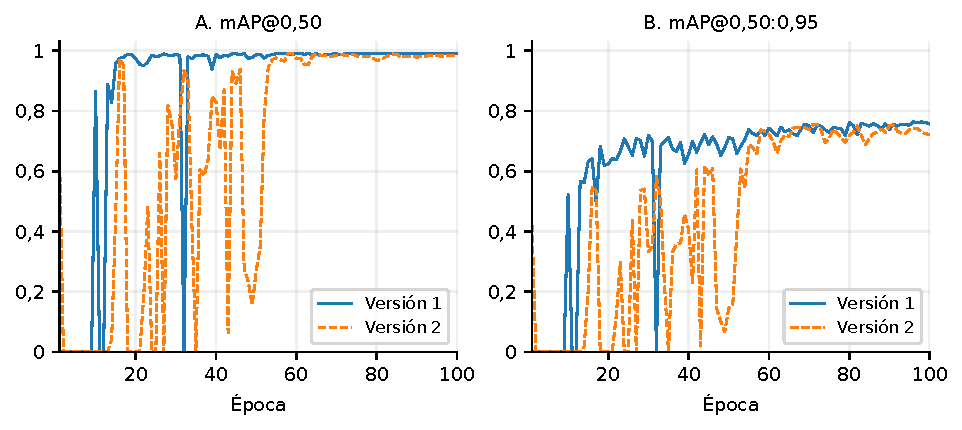
\includegraphics[width=\textwidth]{figures/chapter11/fig11_01_metricas_detector.pdf}
 \caption{Evolución de mAP en los registros de entrenamiento de las dos versiones. Cada punto corresponde a una época. Los registros no constituyen una evaluación adicional del video experimental ni una nueva medición sobre la partición de prueba.}
 \label{fig:curvas-detector}
\end{figure}

Se detectaron valores no numéricos en al menos una pérdida de validación de 11 épocas de la versión 1 y 20 de la versión 2. Las cuatro métricas de detección examinadas contienen valores finitos. Esta incidencia debe conservarse al interpretar el entrenamiento: no se imputaron las pérdidas ni se dedujo su causa a partir del CSV. La información disponible tampoco permite identificar de forma concluyente la época efectiva de \texttt{best.pt}; los cuadros anteriores no se presentan como métricas verificadas de ese archivo de pesos.

\section{Referencia manual y correspondencia temporal}

Las 101 posiciones manuales corresponden a los cuadros 0, 10, 20, hasta 1000. Con 30 FPS, la separación nominal entre anotaciones es de $10/30$ s, aproximadamente $0{,}333$ s. La frecuencia de anotación se distingue de la frecuencia del video. Las filas sin marcación del archivo exportado no se convierten en posiciones ni se rellenan mediante interpolación.

La trayectoria automática abarca los cuadros 0 a 984, con 929 observaciones. La intersección de índices con la referencia contiene 93 cuadros, desde 0 hasta 980. Los cuadros manuales sin posición automática correspondiente son 60, 710, 720, 730, 740, 760, 990 y 1000. Los dos últimos quedan fuera del tramo automático conservado. Las ausencias restantes se encuentran dentro de ese tramo.

La comparación utiliza coincidencia exacta de índice de cuadro. No se asigna una posición automática del cuadro vecino ni se considera un falso positivo cada observación automática sin anotación manual. La referencia es parcial y tiene una resolución temporal menor que el seguimiento. El cociente $93/101$ describe la cobertura de esas anotaciones, no la sensibilidad global del detector ni la exactitud de asociación de identidades.

\section{Alineación del sistema de coordenadas}

Tracker permite definir un origen, una orientación y una escala para transformar posiciones de imagen en coordenadas de análisis \cite{tracker2026}. Por eso, dos recorridos de forma semejante pueden conservar coordenadas numéricas distintas. En el caso estudiado, la coordenada vertical manual aumenta mientras que la coordenada de imagen del modelo disminuye. La semejanza visual se examinó mediante una inversión del sentido de Y y una traslación fijada con el primer par de observaciones.

Las coordenadas iniciales son $(307{,}2;660{,}9)$ para la referencia manual y $(307{,}889282;1667{,}827881)$ para el modelo. Se aplica a todas las anotaciones la transformación
\begin{equation}
 x^{\mathrm{al}}_k=x^{\mathrm{man}}_k,
 \qquad
 y^{\mathrm{al}}_k=C-y^{\mathrm{man}}_k,
 \qquad
 C=y^{\mathrm{mod}}_0+y^{\mathrm{man}}_0
   =2328{,}727881.
 \label{eq:alineacion-tracker}
\end{equation}

El factor de escala permanece en uno; no se rota la trayectoria ni se desplaza X. La constante se obtiene exclusivamente del cuadro 0 y no se reemplaza por la altura del video. En ese cuadro, Y coincide por construcción y persiste una diferencia horizontal aproximada de $0{,}689$ px. Para evaluar los puntos posteriores se excluye el anclaje, de modo que quedan 92 pares entre los cuadros 10 y 980.

Esta operación registra geométricamente la referencia respecto del modelo. No recupera por sí sola la configuración original de Tracker ni establece una equivalencia física con micrómetros. Como utiliza una posición predicha para fijar el origen vertical, los resultados se interpretan como discrepancias después de la alineación, y no como una evaluación independiente de la exactitud absoluta de ese origen.

\section{Comparación de posiciones}

Para cada cuadro común posterior al anclaje se calcula la distancia euclídea entre la posición automática y la manual alineada:
\begin{equation}
 e_k=\sqrt{\bigl(x^{\mathrm{mod}}_k-x^{\mathrm{al}}_k\bigr)^2+
                  \bigl(y^{\mathrm{mod}}_k-y^{\mathrm{al}}_k\bigr)^2}.
 \label{eq:error-posicion-experimental}
\end{equation}
Se resumen su media, mediana, máximo, percentil 95 y raíz del error cuadrático medio, $\mathrm{RMSE}_{p}=\sqrt{\sum_{k=1}^{n}e_k^2/n}$, con $n=92$. No se promedian por separado los errores horizontales y verticales para obtener la media de posición.

\begin{table}[htbp]
 \centering
 \caption{Discrepancia de posición sobre los mismos 92 pares posteriores al anclaje. La comparación directa conserva sistemas de coordenadas incompatibles y se incluye para mostrar el efecto del registro geométrico.}
 \label{tab:errores-posicion}
 \begin{tabular}{@{}lrr@{}}
  \toprule
  Medida (px) & Comparación directa & Referencia alineada \\
  \midrule
  Media & $439{,}120$ & $5{,}328$ \\
  Mediana & $397{,}021$ & $4{,}714$ \\
  RMSE de posición & $507{,}325$ & $6{,}120$ \\
  Percentil 95 & $878{,}154$ & $11{,}338$ \\
  Máximo & $992{,}476$ & $14{,}984$ \\
  \bottomrule
 \end{tabular}
\end{table}

La Figura~\ref{fig:comparacion-tracker} muestra la superposición y las discrepancias por tiempo. De los 92 pares evaluados, 85 tienen una distancia menor o igual que 10 px y los 92 quedan por debajo de 15 px. Estos valores describen la distribución observada; no son tolerancias de aceptación establecidas antes de la prueba. El máximo se encuentra en el cuadro 370, aproximadamente a los $12{,}333$ s.

\begin{figure}[htbp]
 \centering
 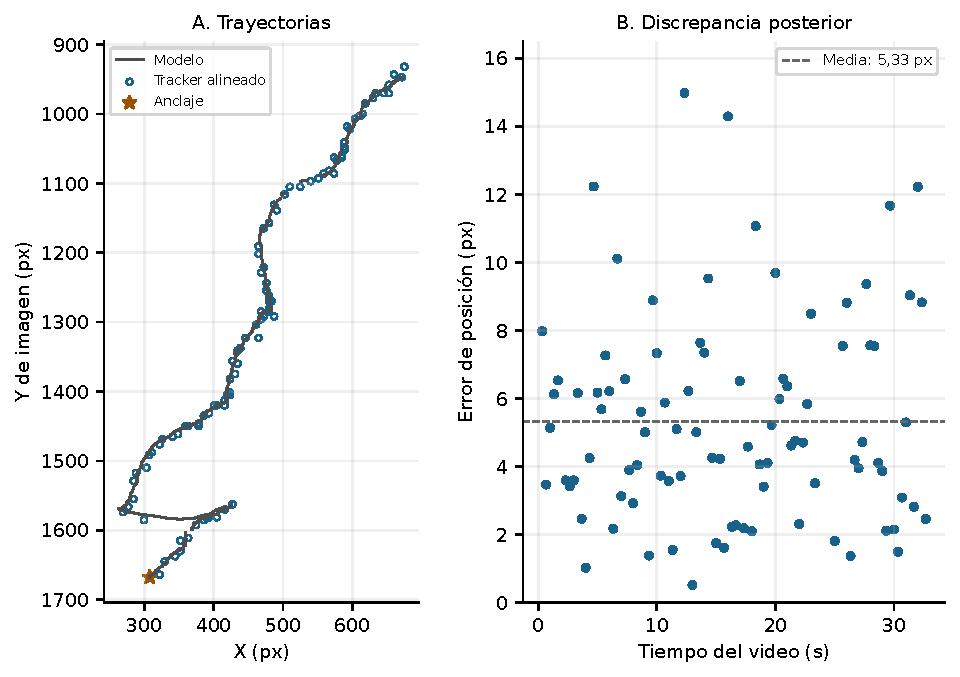
\includegraphics[width=\textwidth]{figures/chapter11/fig11_02_comparacion_trayectorias.pdf}
 \caption{A: posiciones manuales alineadas y trayectoria automática conservada. Los trazos automáticos se interrumpen en los huecos de observación. B: distancia entre posiciones de los mismos cuadros después del anclaje; el cuadro 0 se excluye del resumen. La transformación se mantiene fija para todos los puntos.}
 \label{fig:comparacion-tracker}
\end{figure}

El resultado respalda la similitud geométrica de este par después de la alineación. La comparación directa previa no debe interpretarse como un error de localización de cientos de píxeles atribuible al seguimiento. Aun después del registro persisten diferencias que pueden combinar imprecisión manual, variación del centro de la caja y errores del procesamiento. Una sola anotación por cuadro no permite separar esas contribuciones ni estimar variabilidad entre anotadores.

\section{Continuidad de la trayectoria y observaciones ausentes}

Dentro del intervalo inclusivo de cuadros 0 a 984 hay 985 cuadros posibles y 929 posiciones observadas. La cobertura interna es de aproximadamente $94{,}31$~\%, con 56 cuadros ausentes distribuidos en nueve huecos. El Cuadro~\ref{tab:gaps-experimentales} identifica sus extremos. Los valores se calculan sobre el CSV conservado, sin reconstruir posiciones intermedias.

\begin{table}[htbp]
 \centering
 \caption{Huecos del Track 145. Los extremos son cuadros observados; la cantidad ausente es la diferencia entre extremos menos uno.}
 \label{tab:gaps-experimentales}
 \small
 \begin{tabular}{@{}rrr@{}}
  \toprule
  Último cuadro previo & Primer cuadro posterior & Cuadros ausentes \\
  \midrule
  52 & 54 & 1 \\
  58 & 64 & 5 \\
  694 & 700 & 5 \\
  703 & 722 & 18 \\
  727 & 747 & 19 \\
  759 & 762 & 2 \\
  762 & 764 & 1 \\
  818 & 820 & 1 \\
  821 & 826 & 4 \\
  \midrule
  \multicolumn{2}{@{}l}{Total} & 56 \\
  \bottomrule
 \end{tabular}
\end{table}

Los dos huecos más extensos contienen 18 y 19 cuadros sin observación. La conservación del mismo identificador a ambos lados permite calcular un segmento entre sus extremos, pero no demuestra qué ocurrió durante la ausencia. La pérdida de una posición puede responder a omisión de detección, falta de asociación, oclusión u otras condiciones; el listado de coordenadas no permite asignar una causa visual a cada caso. Tampoco permite contar cambios de identidad ni evaluar cruces de toda la población del video. Esos aspectos quedan pendientes de una revisión específica de imágenes e identidades.

\section{Reconstrucción de las magnitudes de movimiento}

Se aplicaron al CSV las operaciones del capítulo~\ref{chap:analisis-trayectorias}, conservando los índices originales y 30 FPS. El cálculo independiente de distancias, intervalos y cocientes se contrastó con los módulos de rapidez e inspección de la implementación. También coincidieron la media móvil, la clasificación de muestras bajo el umbral de inactividad y las diferencias temporales utilizadas para la variación de rapidez. Esta concordancia verifica la reconstrucción numérica sobre las posiciones disponibles, sin validar nuevamente la inferencia del video.

\begin{table}[htbp]
 \centering
 \caption{Magnitudes reconstruidas del Track 145 completo. La rapidez máxima sin suavizar se distingue del máximo de la media móvil.}
 \label{tab:movimiento-experimental}
 \begin{tabular}{@{}lr@{}}
  \toprule
  Magnitud & Resultado \\
  \midrule
  Tiempo entre primera y última observación & $32{,}8$ s \\
  Distancia acumulada entre observaciones & $1322{,}3331$ px \\
  Desplazamiento neto & $806{,}7973$ px \\
  Rectitud & $0{,}6101$ \\
  Media aritmética de rapideces por segmento & $40{,}2116$ px/s \\
  Rapidez media de trayectoria, distancia/tiempo & $40{,}3150$ px/s \\
  Rapidez máxima por segmento & $403{,}9439$ px/s \\
  Rapidez máxima suavizada & $248{,}2615$ px/s \\
  Muestras suavizadas bajo 30 px/s & $337$ de $909$ \\
  Fracción de muestras suavizadas inactivas & $0{,}3707$ \\
  \bottomrule
 \end{tabular}
\end{table}

La distancia acumulada suma longitudes rectas entre posiciones consecutivas disponibles, incluso al atravesar un hueco. No recupera desplazamientos intermedios no observados. La rapidez por segmento divide cada longitud por su propio intervalo temporal. Por eso, la media de esas rapideces y el cociente entre distancia acumulada y tiempo total son magnitudes diferentes, aunque aquí sus valores sean cercanos.

La media móvil de 20 rapideces produce 909 muestras. De ellas, 337 están estrictamente por debajo de 30 px/s, equivalentes al $37{,}07$~\% de las muestras suavizadas. Este porcentaje no representa directamente una fracción de tiempo ponderada por duración, porque los intervalos no son todos iguales cuando hay huecos. La Figura~\ref{fig:rapidez-experimental} permite examinar la serie original y la suavizada junto con las regiones sin observaciones.

\begin{figure}[htbp]
 \centering
 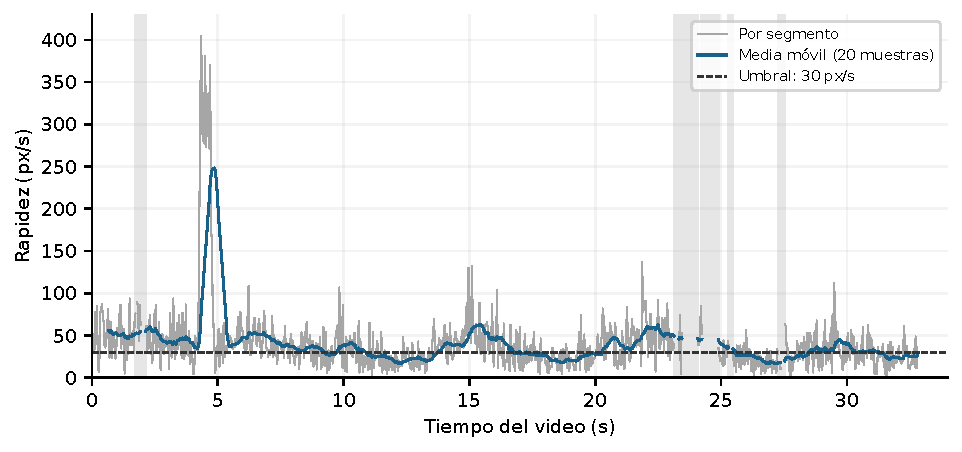
\includegraphics[width=\textwidth]{figures/chapter11/fig11_03_rapidez.pdf}
 \caption{Rapidez por segmento y media móvil de 20 muestras del Track 145. Las regiones grises señalan huecos entre posiciones; las líneas no interpolan esos intervalos. El umbral de 30 px/s se aplica a la serie suavizada para identificar muestras de inactividad.}
 \label{fig:rapidez-experimental}
\end{figure}

Las diferencias temporales de la rapidez suavizada generan 908 valores de variación escalar de rapidez, con extremos de aproximadamente $572{,}53$ y $-553{,}19$ px/s$^2$. Con los umbrales operativos se marcan siete muestras por encima de $450$ px/s$^2$ y cinco por debajo de $-450$ px/s$^2$. La comparación entre medias de ventanas de 50 muestras marca 96 posiciones como posibles cambios de régimen. Las ventanas se solapan: estas cantidades no equivalen a siete, cinco y 96 episodios físicos independientes, ni confirman transiciones biológicas.

\section{Comparación de rapidez con la referencia manual}

La rapidez depende de la resolución temporal con que se observan las posiciones. Para comparar cantidades equivalentes se utilizaron los mismos extremos de los 92 intervalos delimitados por los 93 cuadros comunes. En cada intervalo se calculó la distancia recta entre extremos dividida por el tiempo real, tanto para la referencia alineada como para las posiciones automáticas. En esta comparación no se aplica suavizado ni se suma el recorrido fino del modelo dentro de cada intervalo.

Si $v^{\mathrm{mod}}_j$ y $v^{\mathrm{man}}_j$ son las rapideces del intervalo $j$, se calcularon
\begin{equation}
 \mathrm{MAE}_{v}=\frac{1}{m}\sum_{j=1}^{m}
       \left|v^{\mathrm{mod}}_j-v^{\mathrm{man}}_j\right|,
 \qquad
 \mathrm{RMSE}_{v}=\sqrt{\frac{1}{m}\sum_{j=1}^{m}
       \left(v^{\mathrm{mod}}_j-v^{\mathrm{man}}_j\right)^2},
 \quad m=92.
\end{equation}

El error absoluto medio es de $14{,}0420$ px/s y el RMSE, de $17{,}2047$ px/s. La correlación lineal entre las dos series es de aproximadamente $0{,}8720$. La correlación describe su variación conjunta y no sustituye las medidas de discrepancia. A diferencia de la evaluación de posición, la estimación de los intervalos utiliza también el primer punto como extremo temporal. La inversión y la traslación de Y conservan las distancias entre puntos manuales y, por tanto, sus rapideces; el valor de la constante de alineación no modifica este contraste.

La comparación muestra que la semejanza espacial no implica idéntica precisión al derivar rapidez. Las diferencias entre posiciones de ambos extremos contribuyen al error del desplazamiento y se dividen por un intervalo que suele ser de un tercio de segundo. Además, omitir posiciones intermedias modifica la distancia acumulada: sobre los 93 cuadros comunes, la poligonal automática tiene aproximadamente $1146{,}76$ px, mientras que la referencia manual tiene $1300{,}70$ px. Estos valores corresponden a un tramo y un muestreo diferentes de los 929 puntos del Cuadro~\ref{tab:movimiento-experimental}. No se concluye, a partir de este caso, que la rapidez automática tenga exactitud física suficiente para cualquier uso experimental.

\section{Clasificación posterior del movimiento}

La clasificación estaba desactivada en la corrida original. Para examinar el comportamiento del módulo se aplicó posteriormente el clasificador del capítulo~\ref{chap:clasificacion-movimiento} a las posiciones conservadas, con 30 FPS y sus parámetros predeterminados. Este procedimiento genera una salida nueva de análisis; no se presenta como un archivo de clasificación producido durante aquella inferencia.

El Cuadro~\ref{tab:clasificacion-experimental} muestra las puntuaciones obtenidas sobre la trayectoria completa y sobre las dos secuencias restringidas a los 93 cuadros comunes. Las tres reciben la categoría direccional, aunque sus puntuaciones difieren. El contraste entre la trayectoria completa y su submuestreo muestra que la densidad temporal influye en las características utilizadas por las reglas.

\begin{table}[htbp]
 \centering
 \caption{Puntuaciones del clasificador en el análisis posterior. $Q_D$: direccional; $Q_E$: errático; $Q_C$: circular u oscilatorio. Las puntuaciones son heurísticas, no probabilidades calibradas.}
 \label{tab:clasificacion-experimental}
 \small
 \begin{tabularx}{\textwidth}{@{}Xrccc@{}}
  \toprule
  Secuencia & Puntos & $Q_D$ & $Q_E$ & $Q_C$ \\
  \midrule
  Automática completa & 929 & $0{,}5330$ & $0{,}3497$ & $0{,}5044$ \\
  Automática en cuadros comunes & 93 & $0{,}6186$ & $0{,}1643$ & $0{,}6003$ \\
  Manual alineada en cuadros comunes & 93 & $0{,}5215$ & $0{,}3886$ & $0{,}4706$ \\
  \bottomrule
 \end{tabularx}
\end{table}

En el track completo, la puntuación ganadora supera a la circular u oscilatoria por $0{,}0286$. La asignación es, por tanto, el resultado de la competencia de las reglas y no una afirmación de alta confianza experimental. La rectitud de $0{,}6101$ y la tortuosidad de $0{,}3899$ describen el recorrido observado, pero no identifican un mecanismo físico.

La coincidencia de categoría entre las coordenadas manuales y automáticas aporta una comparación de salidas con el mismo algoritmo. No constituye una validación independiente de la categoría: para medir acierto se requieren etiquetas de referencia asignadas mediante un criterio externo al clasificador. Sin esas etiquetas no se informan exactitud, F1 ni matriz de confusión, ni se considera validada la distinción entre comportamientos direccionales, erráticos y circulares u oscilatorios en la población experimental.

\section{Discusión y alcance de los resultados}

El caso permite vincular una referencia manual parcial con una trayectoria automática y reconstruir sus productos de análisis. La inversión de Y y el anclaje inicial reducen una discrepancia dominada por sistemas de coordenadas incompatibles. Manteniendo fija la transformación, los puntos posteriores conservan una separación media de $5{,}33$ px. Esta evidencia respalda la similitud espacial del par examinado, con las restricciones introducidas por el registro respecto del modelo.

La presencia de huecos no impide obtener métricas con los tiempos reales, pero limita lo que esas métricas representan. La distancia y la rapidez describen conexiones entre observaciones, sin reconstruir el movimiento durante las ausencias. El contraste temporal con Tracker muestra discrepancias de rapidez mayores que las que podría sugerir la superposición visual. Por ello, la validación de posición y la de magnitudes derivadas deben conservarse como evaluaciones diferenciadas.

Los registros de entrenamiento aportan evidencia sobre el detector en las evaluaciones conservadas; no sustituyen una medición de detección sobre el video completo. La referencia de un solo individuo tampoco permite evaluar de forma global conservación de identidad, cruces, oclusiones y fragmentación. La revisión visual específica de esos casos y la disponibilidad de posiciones de otras trayectorias permitirían ampliar la evaluación, sin que la ausencia de ese análisis en este capítulo demuestre ausencia de material experimental.

La clasificación posterior produce resultados inspeccionables, pero su adecuación científica permanece pendiente de comparación con categorías independientes. Los umbrales de inactividad y de cambios de rapidez requieren asimismo una evaluación experimental de su significado, más allá de que el cálculo reproduzca las reglas implementadas.

Las magnitudes se mantienen en px, px/s y px/s$^2$. La alineación con Tracker no determina una escala física. La conversión a micrómetros continúa \textbf{A DEFINIR}, de acuerdo con el alcance establecido en los capítulos metodológicos. Los resultados disponibles permiten documentar la ejecución, su consistencia numérica y una comparación experimental acotada; no justifican todavía generalizaciones a otras condiciones de adquisición o a toda la población de microorganismos.


\backmatter
\printbibliography[heading=bibintoc,title={Bibliografía}]

\cleardoublepage
\thispagestyle{empty}
\begin{center}
  {\Large\bfseries Aval del tribunal\par}
\end{center}

\vspace{1.2cm}

Mediante su firma, los miembros del tribunal de evaluación del Trabajo Especial
\textit{\ThesisTitle}, de \ThesisAuthor, avalan que la versión final presentada
se corresponde con la aprobada por dicho tribunal.

\vspace{0.8cm}
\noindent Fecha: \rule{7cm}{0.4pt}

\vspace{1.8cm}
\noindent\rule{0.46\textwidth}{0.4pt}\hfill\rule{0.46\textwidth}{0.4pt}\\
\noindent\makebox[0.46\textwidth]{Firma y aclaración}\hfill
\makebox[0.46\textwidth]{Firma y aclaración}

\vspace{1.8cm}
\begin{center}
  \rule{0.46\textwidth}{0.4pt}\\
  Firma y aclaración
\end{center}

\vfill
\begin{center}
  \small\textit{Hoja reservada para la versión final. Pendiente del aval y de la firma
  de al menos dos miembros del tribunal (RHCD 572/2024, art. 4).}
\end{center}

\cleardoublepage
\ifThesisFinalLayout
  \hypersetup{pageanchor=false}
  \thesisguardleaf
\fi

\end{document}
